% Chap06 Engineering Applications of the Derivative
\section*{Learning Objectives}
By the end of this chapter, the student should be able to:
\begin{itemize}
    \item Analyze and model engineering problems using the principles of calculus, specifically through the application of derivatives to understand system behaviors.
    \item Develop strategies for solving optimization problems, both with and without constraints.
    \item Critically assess the role of derivatives in determining system dynamics and understand the significance of dynamic equations in engineering contexts.
    \item Apply the concept of energy to the analysis of mechanical systems using the framework of Lagrangian mechanics.
\end{itemize}



\section*{Outcomes}

Upon successful completion of this chapter, students will be able to:
\begin{itemize}
    \item Calculate path length and arc length for given paths.
    \item Solve engineering problems involving root finding and minimization.
    \item Use gradient descent to find local minima of functions and understand its limitations.
    \item Apply second derivative tests to determine the nature of critical points in functions.
    \item Solve optimization problems involving equality and inequality constraints using Lagrange multipliers.
    \item Derive and apply Lagrange’s equations to solve problems in dynamics.
    \item Compute kinetic and potential energy for mechanical systems.
    \item Model and analyze the motion of complex systems like multi-link manipulators using Lagrange’s formalism.
    \item Determine moments of inertia for various bodies and understand their effects on rotational motion.
\end{itemize}

\newpage

\begin{figure}[ht]%
\centering
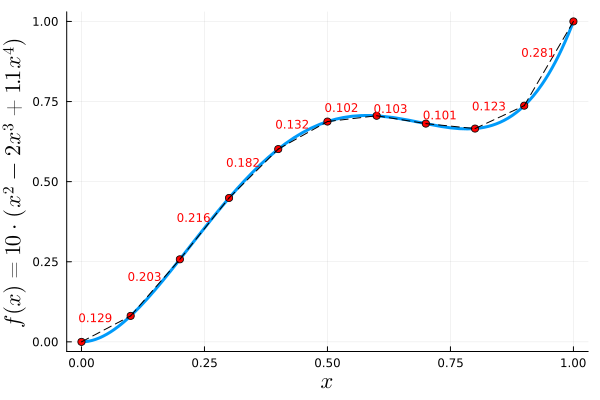
\includegraphics[width=0.7\columnwidth]{graphics/Chap06/pathLength.png}%
    \caption[]{Path length is defined by chopping up the curve into short segments, connecting the endpoints of the segments by straight lines, and then adding up the lengths of the lines. As the segment size tends to zero, the true path length is obtained. Simple? Yes. Useful? Very! It can be used to formulate an important problem: determine a path of shortest length for a robot to travel without hitting obstacles; we'll explore this in homework. Table~\ref{tab:PathLength} shows that the ten segment lengths in the plot add up to 1.572; the true answer, obtained in the limit as the segment lengths shrink to zero and become infinite in number, is $1.5852977678599067 \pm 6.654127165939272e$-$9$. The approximation with ten segments is already quite good!}
    \label{fig:pathLength}
\end{figure}

\begin{table}[ht]
\centering
\caption{Path Length is Easy to Understand but Tedious to Compute by Hand, \\
\centering $S := \int_a^b \sqrt{dx^2 + dy^2} = \int_a^b \sqrt{1 + \left(\frac{dy}{dx}\right)^2 } \, dx ~~(\text{after factoring out}~~dx)$ }
\begin{tabular}{ccc}
\toprule
$x_i$ & $y_i$ & $\sqrt{(x_i - x_{i-1})^2 + (y_i - y_{i-1})^2}$ \\
\midrule
0.0 & 0.0   &  0.0    \\
0.1 & 0.0811 & 0.129 \\
0.2 & 0.2576 & 0.203 \\
0.3 & 0.4491 & 0.216 \\
0.4 & 0.6016 & 0.182 \\
0.5 & 0.6875 & 0.132 \\
0.6 & 0.7056 & 0.102 \\
0.7 & 0.6811 & 0.103 \\
0.8 & 0.6656 & 0.101 \\
0.9 & 0.7371 & 0.123 \\
1.0 & 1.0    & 0.281 \\
\midrule
\multicolumn{2}{r}{$\displaystyle \int_a^b \sqrt{dx^2 + dy^2} \approx \sum_{i=2}^{11} \sqrt{(x_i - x_{i-1})^2 + (y_i - y_{i-1})^2} = $}  & 1.572 \\
\bottomrule
\end{tabular}
\label{tab:PathLength}
\end{table}

\section{Path Length or Arc Length}

You understand the length of a line segment in the plane and the length of the circumference of a circle. But for more complicated curves, what is the length from a point $a$ to a point $b$? Figure~\ref{fig:pathLength} and Table~\ref{tab:PathLength} illustrate the concept of \textbf{arc length (aka, path length)}, which is fundamental in engineering because it allows us to quantify the ``length of a curve'' in the plane \( \mathbb{R}^2 \), which can be defined by a function \( f:(a, b) \to \real \) or parametric equations \( x(t), y(t) \), $t_1 \le t \le t_2$, the arc length is the distance one would travel along the curve between two points.\\

The integral formulas for arc length arise from the Pythagorean theorem. By dividing the curve into infinitesimally small segments, each segment can be approximated by a straight line whose length can be calculated using the Pythagorean theorem as the hypotenuse of a right triangle with sides \( dx \) and \( dy \). As we sum up the lengths of all these segments (a process achieved by integrating), we obtain the total arc length of the curve.



\bigskip

\begin{tcolorbox}[colback=mylightblue, title = {\bf Arc Length = Path Length}, breakable]

\begin{definition} 
\label{def:pathLength} Given a differentiable function \( f : [a, b] \rightarrow \mathbb{R}^2 \), the arc length \( S \) of the curve described by \( y = f(x) \) from \( x=a \) to \( x=b \) is given by the integral, $S:=\int_a^b \sqrt{dx^2 + dy^2}$. After factoring out $dx$, we obtain the standard formula,
\begin{equation}
\label{eq:arclengthFunction}
S = \int_{a}^{b} \sqrt{1 + \left(\frac{dy}{dx}\right)^2} \, dx.
\end{equation}

For a curve defined parametrically by \( x(t) \) and \( y(t) \) where \( t \) ranges from \( t_1 \) to \( t_2 \), the arc length is given by, 
\begin{equation}
\label{eq:arclengthParametricPath}
S = \int_{t_1}^{t_2} \sqrt{\left(\frac{dx}{dt}\right)^2 + \left(\frac{dy}{dt}\right)^2} \, dt.
\end{equation}
\end{definition}
\end{tcolorbox}

\bigskip

\emstat{
\textbf{Notes:} Equation~\ref{eq:arclengthParametricPath} is the more general formula for computing path length. When the path is given by a function, as in $(x, y(x))$, \eqref{eq:arclengthFunction} follows from \eqref{eq:arclengthParametricPath} as shown below:
\begin{align*}
    S &= \int_{a=x(t_1)}^{b = x(t_2)} \sqrt{\left(\frac{dx}{dt}\right)^2 + \left(\frac{dy}{dt}\right)^2} \, dt  ~~(\text{factor out}~~\left(\frac{dx}{dt}\right)^2) \\[1em]
    &= \int_{a=x(t_1)}^{b = x(t_2)} \sqrt{  1 + \left( \frac{\frac{dy}{dt} }{ \frac{dx}{dt} }\right)^2 } \, ~~\left(\frac{dx}{dt}\right) \, dt  ~~(\text{cancel the }~~dt's) \\[1em]
    & = \int_{a}^{b}  \sqrt{1 + \left(\frac{dy}{dx}\right)^2} \, dx.
\end{align*}

\textbf{Source of the formula for arc length:} Figure~\ref{fig:pathLength} and Table~\ref{tab:PathLength} provide the basic idea. Let $\Delta x$ and $\Delta y$ be incremental changes in $x$ and $y$ along a curve. Then the distance covered is given by the Pythagorean Theorem, $\Delta S:= \sqrt{(\Delta x)^2 + (\Delta y)^2}$. Taking the limit as $\Delta x$ goes to zero, we obtain $dS = \sqrt{(dx)^2 + (dy)^2}$, and hence
$$S = \int_a^b dS =\int_a^b \sqrt{(dx)^2 + (dy)^2}. $$
But hmmm, we have never seen an integral like this! Suppose that the $(x,y)$ coordinates of the curve are parameterized by time. Then, using the linearization (aka, first-order Taylor expansion), we have
\begin{align*}
    \Delta x &= x(t + \Delta t) - x(t)  \underset{{\Delta t \to 0}}\longrightarrow \left( \frac{dx(t)}{dt}\right) \cdot dt \\[1em]
    \Delta y &= y(t + \Delta t) - y(t)  \underset{{\Delta t \to 0}}\longrightarrow \left( \frac{dy(t)}{dt}\right) \cdot dt 
\end{align*}
Substituting into the previous equation and factoring out $dt$ gives the result.

}



\bigskip

\begin{example} (Classical Example because the Integral is Easy to Evaluate). A circle of radius $r>0$ about the origin can be parameterized by $\left(x(t) = r \sin(t), y(t) = r \cos(t)\right)$, for $0 \le t \le 2 \pi$. Compute the arc length from $t_1 = \pi/3$ to $t_2 = \pi$.

\end{example}

\solution \Ans $S = 2 r \frac{\pi}{3}$.\\

We apply \eqref{eq:arclengthParametricPath}. 
\begin{itemize}
    \item $x(t) = r \sin(t) \implies \frac{dx}{dt} = r \cos(t)$.
    \item $y(t) = r \cos(t) \implies \frac{dy}{dt} = -r \sin(t)$.
    \item $\sqrt{\left(\frac{dx}{dt}\right)^2 + \left(\frac{dy}{dt}\right)^2} = r$.
\end{itemize}
Hence,
$$S = \int_{t_1}^{t_2} \sqrt{\left(\frac{dx}{dt}\right)^2 + \left(\frac{dy}{dt}\right)^2} \, dt = \int_{\pi/3}^\pi r \, dt = r \cdot t \Big|_{\pi/3}^\pi = r \left( \pi - \pi/3\right)  = 2 r \pi/3.  $$




\Qed




\bigskip
\begin{example}
Compute the path length of the curve defined by \( y = f(x) = x^2 \) from \( x=0 \) to \( x=1 \). 
\end{example}

\solution \Ans $S = 1.479$.\\

The derivative \( \frac{dy}{dx} \) is \( 2x \). Hence, the arc length is calculated as:
\begin{equation}
S = \int_{0}^{1} \sqrt{1 + (2x)^2} \, dx.
\end{equation}
Setting up the integral is the main skill to be mastered here. In Chapter~\ref{chap:AntiDerivFundThmCalc}, we'll learn how to compute closed-form solutions\footnote{$S = \int_{0}^{1} \sqrt{1 + (2x)^2} \, dx =  \int_{0}^{2} \sqrt{1 + u^2} \, \frac{du}{2} = \frac{1}{2} \int_{0}^{2} \sqrt{1 + u^2} \, du = \asinh(u) \Big|_0^2 =  \frac{1}{2} \asinh(2)$,} for such integrals when the function defining the path is simple enough, such as $f(x) = x^2$. For now, we seek a numerical answer, which is what real engineers must do in 99.9\% of cases.

\bigskip

\begin{lstlisting}[language=Julia,style=mystyle]
using QuadGK

# Define the function for the curve
f(x) = x^2

# Define the derivative of the function
df(x) = 2x

# Define the integrand for arc length
function arc_length_integrand(x)
    return sqrt(1 + df(x)^2)
end

# Compute the arc length using QuadGK
integral, error = quadgk(arc_length_integrand, 0, 1)

println("The arc length of the curve from x = 0 to x = 1 is approximately: ", integral)
println("The estimated error of the computation is: ", error)

\end{lstlisting}
\textbf{Output} 
\begin{verbatim}
The arc length of the curve from x = 0 to x = 1 is approximately: 1.4789428575446002

The estimated error of the computation is: 1.0424397123287577e-8
\end{verbatim}
\Qed

\bigskip


\begin{example}
Compute the arc length of the curve defined by \( y = f(x) = 10(x^2 - 2x^3 + 1.1x^4) \) from \( x=0 \) to \( x=1 \). 
\end{example}

\solution \Ans $S = 1.585$.\\

The derivative \( \frac{dy}{dx} \) is \( 10(2x - 6x^2 + 4.4x^3)
 \). Hence, the arc length is calculated as:
\begin{equation}
S = \int_{0}^{1} \sqrt{1 + \left( 10(2x - 6x^2 + 4.4x^3) \right)^2} \, dx.
\end{equation}
Try as one may with techniques to be developed in Chapter~\ref{chap:AntiDerivFundThmCalc}, computing a closed-form solution to the integral is likely impossible. In any case, neither ChatGPT nor your author is able to do it! For QuadGK, it is cake:

\begin{lstlisting}[language=Julia,style=mystyle]
using QuadGK

# Define the function for the curve
f(x) = 10*(x^2 - 2*x^3 + 1.1*x^4)

# Define the derivative of the function
df(x) = 10*(2x - 6x^2 + 4.4x^3)

# Define the integrand for arc length
function arc_length_integrand(x)
    return sqrt(1 + df(x)^2)
end

# Compute the arc length using QuadGK
integral, error = quadgk(arc_length_integrand, 0, 1)

println("The arc length of the curve from x = 0 to x = 1 is approximately: ", integral)

println("The estimated error of the computation is: ", error)
\end{lstlisting}
\textbf{Output} 
\begin{verbatim}
The arc length of the curve from x = 0 to x = 1 is approximately: 1.5852977678599067

The estimated error of the computation is: 6.654127165939272e-9
\end{verbatim}
\Qed

\bigskip

\begin{figure}[htb]%
\centering
\hfill% 
\subfloat[]{%
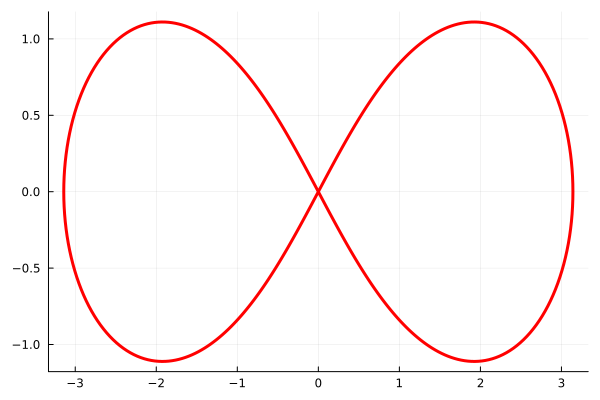
\includegraphics[width=0.43\columnwidth]
{graphics/Chap06/figureEight.png}}%
\hfill%
\subfloat[]{%
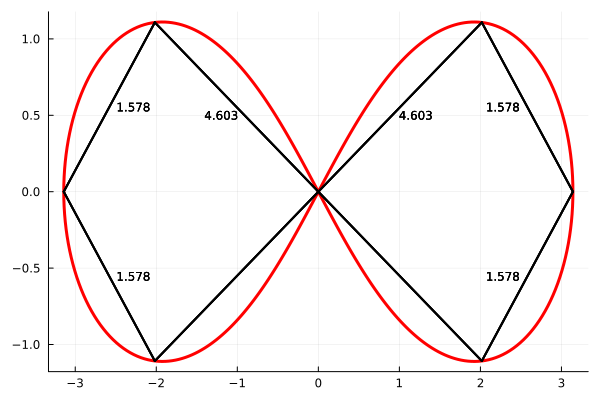
\includegraphics[width=0.43\columnwidth]{graphics/Chap06/figureEightCrudelyEstimatedPathLength.png}}%
\hfill
\caption[]{A figure eight is clearly not a function from $x$ to $y$. (a) Rather, it is a parameterized curve in the plane. Example~\ref{ex:figureEight} explains what is going on. (b) Shows a very crude straight line underapproximation of the arc length yielding $S \approx 4 \cdot (1.578) + 2 \cdot(4.603) = 15.518$. How far do you think it is off? The two lines of length 4.603 cross through the origin to hit the other side of the figure.}
    \label{fig:figureEightPathLength}
\end{figure}

\begin{example}
\label{ex:figureEight}
Figure~\ref{fig:figureEightPathLength} depicts a figure eight parameterized by 
\begin{align*}
    x(t) &= \pi \cdot \frac{\cos\left(\frac{t \cdot 2\pi}{4}\right)}{1 + \sin^2\left(\frac{t \cdot 2\pi}{4}\right)} \\[1em]
    y(t) & = \pi \cdot \frac{\sin\left(\frac{t \cdot 2\pi}{4}\right) \cdot \cos\left(\frac{t \cdot 2\pi}{4}\right)}{1 + \sin^2\left(\frac{t \cdot 2\pi}{4}\right)}
\end{align*}
for $0 \le t \le 4$. Compute its arc length.    
\end{example}

\solution \Ans $S = 16.47$\\

This time, the path in $\real^2$ is not specified by a function, but instead by a parameterized curve $(x(t), y(t))$,  $0 \le t \le 4$. This is more general than a function because the curve can cross itself, fail the vertical line test, and do all sorts of crazy and wonderful things, just like a drone flying in the air. To compute arc length, we need to apply the formula 
$$
S = \int_{t_1}^{t_2} \sqrt{\left(\frac{dx}{dt}\right)^2 + \left(\frac{dy}{dt}\right)^2} \, dt = \int_{t_1}^{t_2} \sqrt{ \left( {x}'(t) \right)^2 + \left({y}'(t)\right)^2 } \, dt.$$

We compute the derivatives using software and obtain
\begin{align*}
    {x}'(t) &= -\frac{\pi \cdot 2\pi \cdot \sin\left(\frac{2\pi t}{4}\right)}{4 \cdot \left(\sin^2\left(\frac{2\pi t}{4}\right) + 1\right)} - \frac{\pi \cdot 4\pi \cdot \sin\left(\frac{2\pi t}{4}\right) \cdot \cos^2\left(\frac{2\pi t}{4}\right)}{4 \cdot \left(\sin^2\left(\frac{2\pi t}{4}\right) + 1\right)^2}\\[1em]
   {y}'(t) & = -\frac{\pi \cdot 2\pi \cdot \sin^2\left(\frac{2\pi t}{4}\right)}{4 \cdot \left(\sin^2\left(\frac{2\pi t}{4}\right) + 1\right)} + \frac{\pi \cdot 2\pi \cdot \cos^2\left(\frac{2\pi t}{4}\right)}{4 \cdot \left(\sin^2\left(\frac{2\pi t}{4}\right) + 1\right)} - \frac{\pi \cdot 4\pi \cdot \sin^2\left(\frac{2\pi t}{4}\right) \cdot \cos^2\left(\frac{2\pi t}{4}\right)}{4 \cdot \left(\sin^2\left(\frac{2\pi t}{4}\right) + 1\right)^2}
\end{align*}

We're all set now to do the integral numerically.

\begin{lstlisting}[language=Julia,style=mystyle]
# Figure 8 
using QuadGK, Plots, LaTeXStrings

function x_position(t)
    a = pi; T = 4
    a * cos(t*2*π/T) / (1 + sin(t*2*π/T)^2)
end
function y_position(t)
    a = pi; T = 4
    a * sin(t*2*π/T) * cos(t*2*π/T) / (1 + sin(t*2*π/T)^2)
end

# Compute the arc length

# Derivatives
function dx_dt(t)
     a = pi; T = 4
    -2*π*a*sin(2*π*t/T)/(T*(sin(2*π*t/T)^2 + 1)) - 4*π*a*sin(2*π*t/T)*cos(2*π*t/T)^2/(T*(sin(2*π*t/T)^2 + 1)^2)
end

function dy_dt(t)
     a = pi; T = 4
    -2*π*a*sin(2*π*t/T)^2/(T*(sin(2*π*t/T)^2 + 1)) + 2*π*a*cos(2*π*t/T)^2/(T*(sin(2*π*t/T)^2 + 1)) - 4*π*a*sin(2*π*t/T)^2*cos(2*π*t/T)^2/(T*(sin(2*π*t/T)^2 + 1)^2)
end

# Define the integrand for arc length
function arc_length_integrand(t)
    return sqrt(dx_dt(t)^2 + dy_dt(t)^2)
end

# Compute the arc length using QuadGK
integral, error = quadgk(arc_length_integrand, 0, 4)

println("The arc length of the curve from x = 0 to x = 4 is approximately: ", integral)
println("The estimated error of the computation is: ", error)

# make a nice plot

dt = 0.01
t = collect(0.0:dt:4.0)
xvalues = x_position.(t)
yvalues = y_position.(t)

p1 = plot(xvalues, yvalues, lw=3, color=:red, apect_ratio = 1, gudefont = 15, label=false)
\end{lstlisting}
\textbf{Output} 
\begin{verbatim}
The arc length of the curve from x = 0 to x = 4 is approximately: 16.474873499707456

The estimated error of the computation is: 1.5850782530968388e-7
\end{verbatim}
Hence, the very crude approximation in Figure~\ref{fig:figureEightPathLength}-(b) is off by about 10\%. 
\Qed

\bigskip


\emstat{{\bf Helpful videos:} Keep in mind that setting up the integral is the main thing to master. Once you have the problem properly formulated, then you can employ software tools to find the answer.\\

\begin{itemize}
    \item \href{https://youtu.be/PK7HZiFG_VI}{Arc Length (formula explained)} by \bprp.
    \item \href{https://youtu.be/8Y-snjheI9M}{Arc length intro | Applications of definite integrals} by the Khan Academy.
    \item \href{https://youtu.be/fh_TPlcGeIo}{Find the Arc Length of a Function with Calculus} by Quoc Dat Phung. Positive: He has strong graphics. Negative: He uses manual integration instead of numerical integration. We cover how to manually compute similar integrals in Chapter~\ref{chap:AntiDerivFundThmCalc}. For now, just watch how he sets up the problems.
    \item \href{https://youtu.be/DNDAwWIL5FY}{Arc Length Calculus Problems} by the Organic Chemistry Tutor. 
\end{itemize}
}



\section{Root Finding and Unconstrained Minimization}

The methods of this section are grounded in the linear approximation of a nonlinear function developed in Prop.~\ref{thm:LinearApproxMultiVariable}. Root finding uses
$$
    f(x) \approx f(x_0) + \frac{\partial f(x_0)}{\partial x} \cdot (x - x_0),~~~~f:\real^n \to \real^n, \\
$$
while minimization uses the equivalent form developed in \eqref{eq:GradLinearization},
$$
    f(x) \approx f(x_0) + \nabla f(x_0) \bullet (x - x_0),~~~~f:\real^n \to \real, \\
$$
where the heavy dot, $\bullet$, denotes the dot product of two column vectors.

\subsection{Root Finding}

We consider a function $f:\real^n \to \real^n$ and seek a \textbf{root, that is, a point $\bf{x_0 \in \real^n}$ such that $\bf{f(x_0)=0}$}. Note that the domain and range are both $\real^n$, and thus, this is the nonlinear equivalent of solving a square linear system of equations, $Ax-b=0$. We recall that $\det(A)\neq 0$ is the magic condition for the existence and uniqueness of solutions to $Ax-b=0$. \\

Suppose that $x_k$ is the current guess for a root. Recall from ROB 101 \textit{Computational Linear Algebra} that the \textbf{Newton-Raphson Algorithm} uses the linear approximation of $f$ about the point $x_k$ to choose $x_{k+1}$ so that $f(x_{k+1})\approx 0$.  In other symbols, $x_{k+1}$ should satisfy,
\begin{equation}
    \label{eq:NewtonMethodVector01}
    0 = f(x_{k+1}) \approx f(x_k) + \frac{\partial f(x_k)}{\partial x}\cdot (x_{k+1)} - x_k),
\end{equation}
which is equivalent to
\begin{equation}
    \label{eq:BasicNewtonRaphson}
       0  \approx f(x_k) + \frac{\partial f(x_k)}{\partial x}\cdot (x_{k+1} - x_k).
\end{equation}
If the Jacobian $\frac{\partial f(x_k)}{\partial x}$ is invertible, and the approximation sign is replaced with an equals sign, a unique value for $x_{k+1}$ is obtained. Solving this equation iteratively yields the Newton-Raphson Algorithm.

\vspace*{0.2cm}
\begin{methodColor}{Newton-Raphson Algorithm}{{NewtonRaphsonAlgorithm}}
    Based on \eqref{eq:BasicNewtonRaphson}, we define\footnote{Note that $\Delta x_k = x_{k+1}-x_k$.} $x_{k+1}:= x_k + \Delta x_k$, where $ \Delta x_k$ is our update to $x_k$. We can then break the algorithm into two steps,
\begin{align}
\label{eq:NewtonRaphsonStep1}
\left(\frac{\partial f(x_k)}{\partial x} \right) \Delta x_{k} &= - f(x_k) \hspace*{0.58cm}(\text{solve for}~~\Delta x_k)  \\
\label{eq:NewtonRaphsonStep2}
x_{k+1}&= x_k + \Delta x_{k}~~(\text{use~~} \Delta x_k ~~\text{to update our estimate of the root}).
\end{align}
While for toy problems, one can use the matrix inverse to solve \eqref{eq:NewtonRaphsonStep1} for $\Delta x_{k}$, for larger problems, one uses LU Factorization or QR Factorization. Once \eqref{eq:NewtonRaphsonStep1} has been solved, $x_{k+1}$ is updated in \eqref{eq:NewtonRaphsonStep2} and the process repeats.\\

A \textbf{damped Newton-Raphson Algorithm} is obtained by replacing \eqref{eq:NewtonRaphsonStep2} with   
\begin{equation}
    \label{eq:NewtonRaphsonStep3}
x_{k+1}= x_k + \epsilon \Delta x_{k},
\end{equation}
for some $\epsilon >0$.
 The validity of the Newton-Raphson Algorithm rests upon: 
\begin{itemize}
    \item the function $f$ being differentiable;
    \item the Jacobian $\frac{\partial f(x_k)}{ \partial x}$ having a non-zero determinant at points generated by \eqref{eq:NewtonRaphsonStep1} and \eqref{eq:NewtonRaphsonStep2}; and
    \item \fbox{the linear equation $f_{\rm lin}(x) = f(x_k) + \frac{\partial f(x_k)}{ \partial x} (x - x_k) $ being a good approximation to the nonlinear function, $f(x)$.}
\end{itemize}
\end{methodColor}

You can find in Chapter 11 of ROB 101 \textit{Computational Linear Algebra} numerous examples with a hand-made implementation of the Newton-Raphson Algorithm. Hence, here, the focus is on Julia Packages. We suggest  \href{https://github.com/JuliaNLSolvers/NLsolve.jl}{NLsolve.jl}, which is based on Newton-Raphson and important variations of the same.

\subsubsection{using NLsolve}

\begin{lstlisting}[language=Julia,style=mystyle]
# Import the NLsolve package
using NLsolve

# This script aims to solve a system of nonlinear equations using the Newton-Raphson method provided by the NLsolve package.

# Define the system of nonlinear equations.
# The function `system_of_equations!` modifies the input array `F` to represent the system of equations.
# The system to be solved is:
# 1) x[1]^2 + x[2]^2 = 2.0
# 2) x[1]^2 - x[2]^2 = 1.0
# 
# Parameters:
# - F: An array that will be modified in-place to represent the system of equations.
# - x: An array representing the variables of the system.
function system_of_equations!(F, x)
    F[1] = x[1]^2 + x[2]^2 - 2.0  # First equation
    F[2] = x[1]^2 - x[2]^2 - 1.0  # Second equation
end

# Provide an initial guess for the solution. 
# The quality of the initial guess can influence the convergence of the Newton-Raphson method.
# In this case, both x[1] and x[2] are initially guessed to be 1.0.
initial_guess = [1.0, 1.0]

# Use the `nlsolve` function from the NLsolve package to find the roots of the system.
# The function returns a result object that contains various information about the solution process.
result = nlsolve(system_of_equations!, initial_guess)

# Print the roots (solutions) of the system.
println("Roots found at: ", result.zero)

\end{lstlisting}
\textbf{Output} 
\begin{verbatim}
Roots found at: [1.2247448713915894, 0.7071067811873448]
\end{verbatim}

\bigskip

As you can see from the code, it aims to find the roots of the system of equations,
\begin{align*}
x_1^2 + x_2^2 &= 2 \\
x_1^2 - x_2^2 &= 1.
\end{align*}
In Julia, the `bang'' notation, denoted by an exclamation mark (\texttt{!}) at the end of a function name, is a convention used to indicate that the function may modify its arguments in-place. This convention is not enforced by the language itself but is widely adopted in the Julia community to signal the side effects of a function. 

For example, consider the function,
\begin{verbatim}
function system_of_equations!(F, x)
    F[1] = x[1]^2 + x[2]^2 - 2.0
    F[2] = x[1]^2 - x[2]^2 - 1.0
end
\end{verbatim}
The presence of the \texttt{!} in the function name \texttt{system\_of\_equations!} suggests that the function might modify the contents of the arguments \texttt{F} and/or \texttt{x} directly, rather than returning a new modified value.
\textbf{Modifying arguments in place can be more memory efficient}, especially for large data structures, as it avoids the need to allocate new memory for the returned values. This can lead to performance benefits in many scenarios, especially in iterative algorithms where the same operation is performed multiple times. However, it's essential to use this convention judiciously. \textbf{Modifying arguments in place can make code harder to understand and debug if not used carefully. } 

\bigskip
\textbf{You are NOT obliged to use modification in place.} Here is the same example using simpler programming constructs.
\bigskip

\begin{lstlisting}[language=Julia,style=mystyle]
using NLsolve

# Define the system of nonlinear equations WITHOUT
# using modification in place
function system_of_equations(x)
    return [
        x[1]^2 + x[2]^2 - 2.0,
        x[1]^2 - x[2]^2 - 1.0
    ]
end

# Initial guess for the solution
initial_guess = [1.0, 1.0]

# Solve the system of equations
result = nlsolve(system_of_equations, initial_guess)

# Print the solution
println("Roots found at: ", result.zero)
\end{lstlisting}
\textbf{Output} 
\begin{verbatim}
Roots found at: [1.2247448713915894, 0.7071067811873448]
\end{verbatim}

\bigskip
Here is a more impressive example of root finding, where we would NOT want to solve these equations by hand.
\bigskip

\begin{lstlisting}[language=Julia,style=mystyle]
using NLsolve
using Random
Random.seed!(1958)

function Fun!(Fun, x)
    Fun[1] = x[1]^2 + x[2] - x[3] + x[4]^3 - 10
    Fun[2] = x[2]^2 + x[5] - x[6] + x[7]^2 - 20
    Fun[3] = x[3]^2 + x[8] - x[9] + x[1]^2 - 30
    Fun[4] = x[4]^2 + x[5]^3 - x[6] + x[9] - 40
    Fun[5] = x[7]^2 + x[8]^3 - x[9] + x[2] - 50
    Fun[6] = x[1] + x[2]^2 - x[3]^3 + x[4] - 5
    Fun[7] = x[5] + x[6]^2 - x[7]^3 + x[8] - 15
    Fun[8] = x[9] + x[1]^2 - x[2]^3 + x[3] - 25
    Fun[9] = x[4] + x[5]^2 - x[6]^3 + x[7] - 35
end

# Trying a different initial guess
x0 = randn(9) * 10

# Adjust solver settings
result = nlsolve(Fun!, x0, method = :trust_region, ftol = 1e-10, 
xtol = 1e-10, iterations = 10000)

println("Roots found at: ", result.zero)
println(" ")

# After obtaining result from nlsolve
Fun_evaluated = Vector{Float64}(undef, length(x0))
Fun!(Fun_evaluated, result.zero)
println("Values of Fun at the root: ", Fun_evaluated)
\end{lstlisting}
\textbf{Output} 
\begin{verbatim}
Roots found at: [-7.772786278382927, 4.157370417426024, 0.9040581712865199, -3.7720366206105242, -2.352593029768065, -3.258024109655881, -1.3456746012402663, 4.301070357560675, 35.53459806404852]
 
Values of Fun at the root: [7.105427357601002e-15, -3.552713678800501e-15, 3.552713678800501e-15, 7.105427357601002e-15, 2.1316282072803006e-14, -3.552713678800501e-15, 0.0, 2.4868995751603507e-14, -7.105427357601002e-15]
\end{verbatim}


% \begin{figure}[htb]%
% \centering
% \subfloat[]{%
% 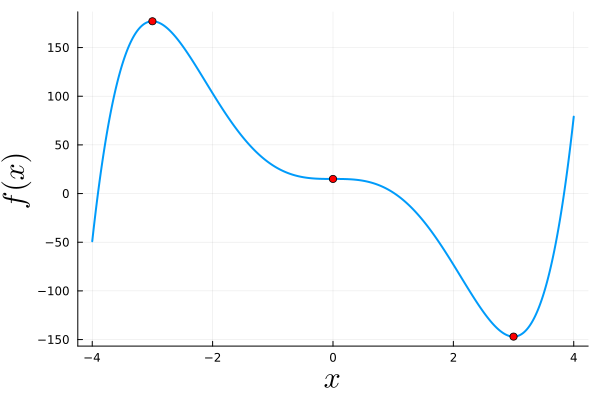
\includegraphics[width=0.6\columnwidth]{graphics/Chap06/scalarFunctionWithLocalMinMaxInflection.png}}%
% \newline
% \subfloat[]{%
% 	%\centering
%  \hspace{-25pt}
% 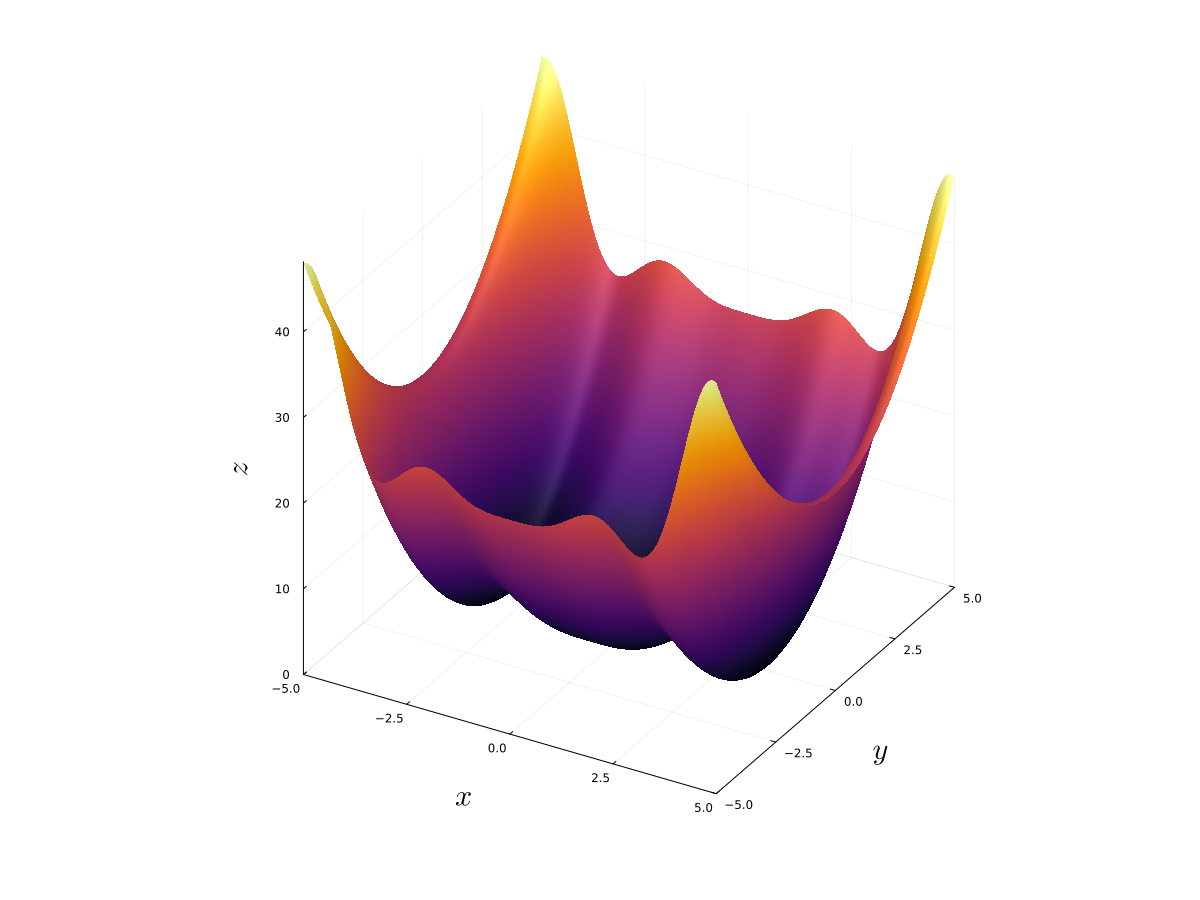
\includegraphics[width=0.45\columnwidth]{graphics/Chap06/2DfunctionWithManyLocalMinMax.png}}%
% \hspace{35pt}
% \hfill%
% \subfloat[]{%
% 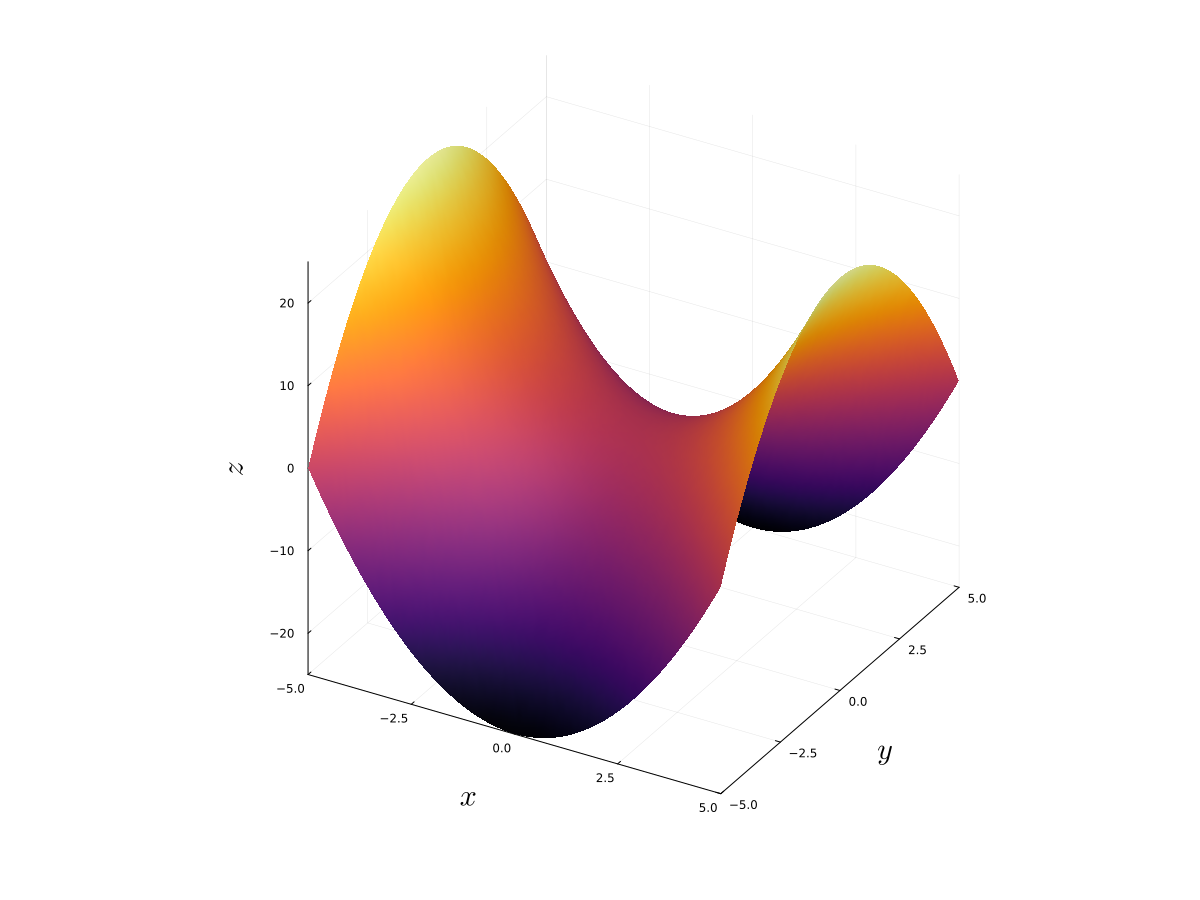
\includegraphics[width=0.45\columnwidth]{graphics/Chap06/2DFunctionWithSaddlePoint.png}}%
% \hfill
%     \caption[]{Blah blah }
%     \label{fig:OptimizationVocabularyVisualized}
% \end{figure}

\begin{figure}[htb]%
\centering
\subfloat[]{%
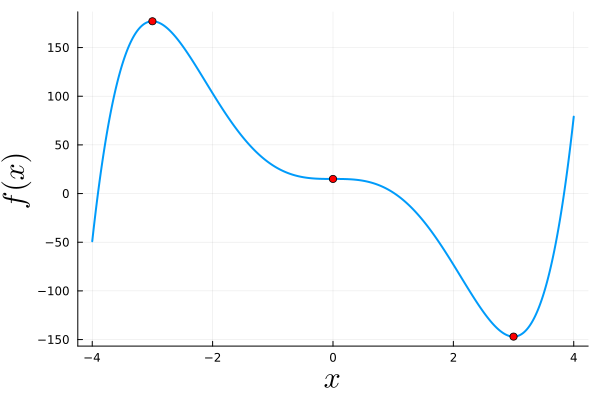
\includegraphics[width=0.5\columnwidth]{graphics/Chap06/scalarFunctionWithLocalMinMaxInflection.png}}%
\newline
\subfloat[]{%
 \hspace{-15pt}
%\includegraphics[trim=left2 bottom2 right2 top2, clip, width=0.5\columnwidth]
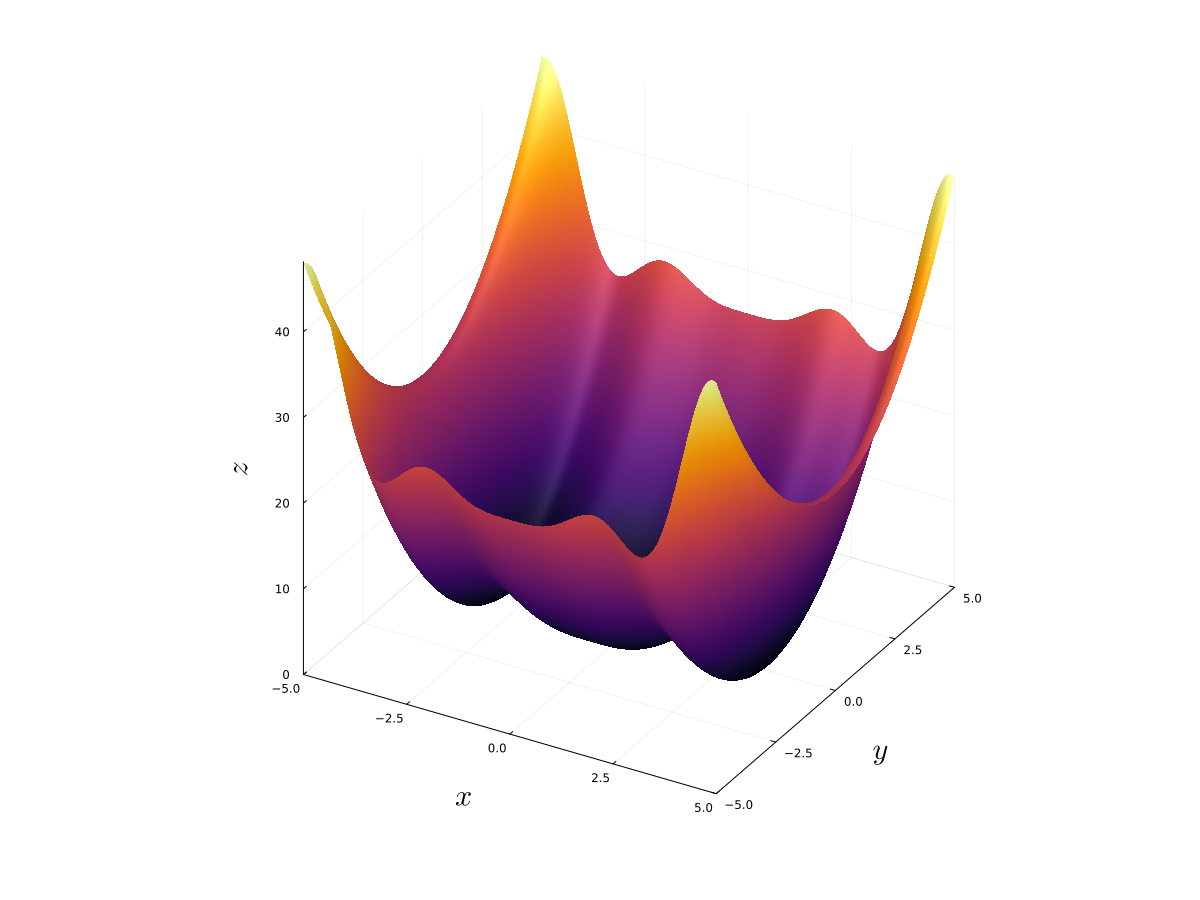
\includegraphics[trim=7cm 1cm 7cm 1cm, clip, width=0.45\columnwidth]{graphics/Chap06/2DfunctionWithManyLocalMinMax.png}}%
\hspace{20pt}
\hfill%
\subfloat[]{%
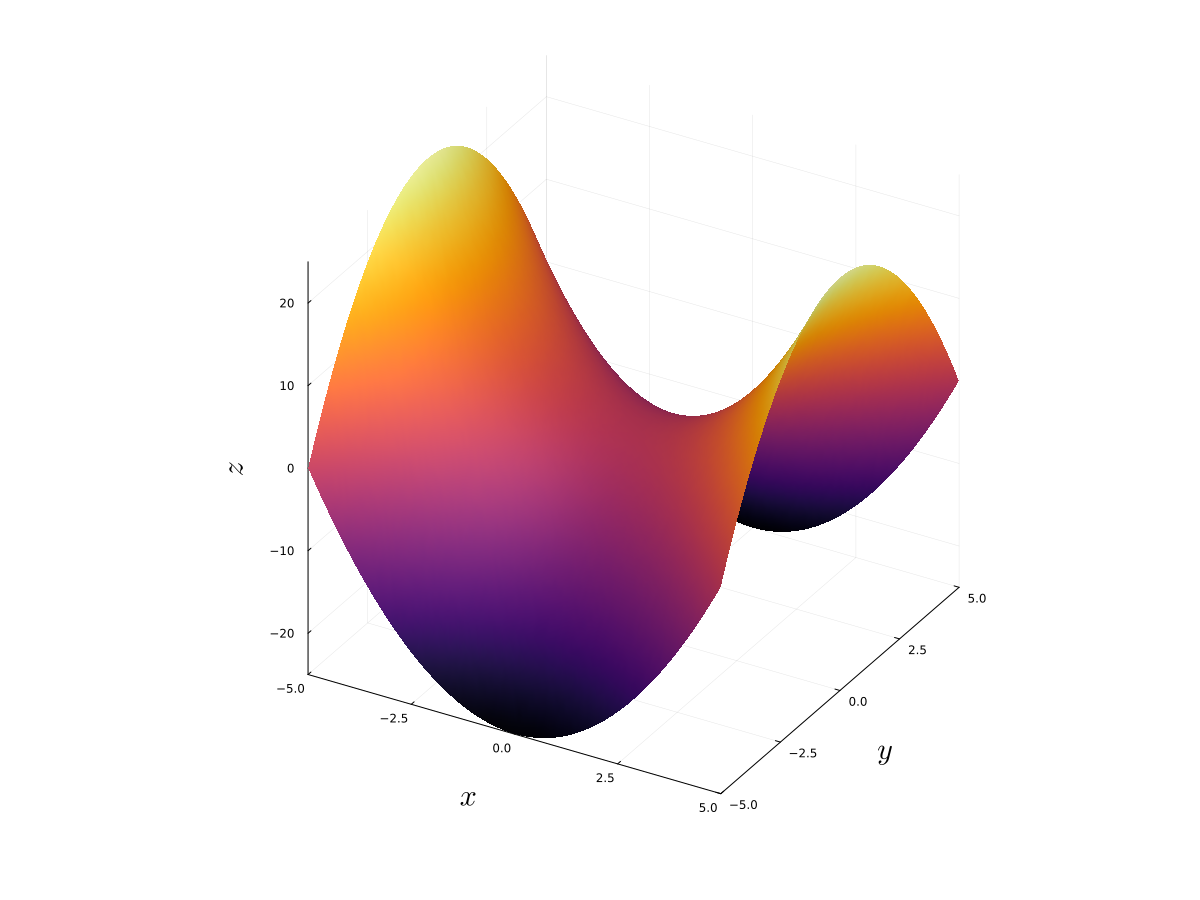
\includegraphics[trim=7cm 1cm 7cm 1cm, clip, width=0.45\columnwidth]{graphics/Chap06/2DFunctionWithSaddlePoint.png}}%
\hfill
    \caption[]{Three cost functions. (a) $f(x) = x^5 - 15x^3 + 15$ has a local minimum at $-3$, an inflection point at the origin, and a local maximum at $3$. (b) $f(x, y) = (x\cdot \sin(x))^2 + y^2$ is riddled with local minima and maxima. (c) $f(x, y) = x^2 - y^2$ has a saddle point at the origin. The name could not be more clear!}
    \label{fig:OptimizationVocabularyVisualized}
\end{figure}

\FloatBarrier

\subsection{Minimization without Constraints}
\label{sec:MinNoConstraints}

Optimization is the process of finding one or more values $x\in \real^n$ that \textbf{minimize a function} $f: \real^n \to \real,$ 
where the scalar-valued function $f$ is called the \textbf{cost function}. The cost function should be designed such that it has a minimum at a point $x^\ast$ that is of interest to you, it should be ``small'' for values of $x$ that are ``near'' $x^\ast$, and it should be ``large'' for values of $x$ that are ``far'' from your preferred value, $x^\ast$. In other symbols, the function should be `` bowl-shaped'' like $f(x) = (x - x^\ast)^2$. You may recall from Chapter 12 of ROB 101 \textit{Computational Linear Algebra}, in Machine Learning, a cost function for minimization is also called a \textbf{regret function} in the sense that you regret being far from your preferred value, $x^\ast$, and your regret is minimum at $x^\ast$. We will abuse notation\footnote{Abusing notation means that one is being a bit sloppy with one's use of symbols, which is what notation is! One often abuses notation when doing the right thing is painful and would cause more of a distraction to explain the good notation than to caution about using poor notation!} and write
\begin{equation}
    \label{eq:ArgMinAbuseNotation}
    x^\ast = \argmin_{x\in \real^n} f(x)
\end{equation}
to denote the value of $x$ achieving the minimum, even when there may be more than one such $x$.\\

One can also do the opposite of minimization, which is to \textbf{maximize a cost function}. In this case, the Machine Learning community calls the cost function a \textbf{reward}, because hey, who does not like to maximize reward and minimize regret! We will stick to minimization throughout this section because  
$$ \argmax_{x\in \real^n} f(x) = \argmin_{x\in \real^n} \left( -f(x) \right),$$
that is, by a simple sign change, you convert a maximization problem into a minimization problem. Most of the numerical packages take advantage of this property. 


\subsubsection{Fundamental Idea and Vocabulary}

Because the gradient is the transpose of the Jacobian, the linearization of $f$ via the gradient can be written as 
\begin{equation}
\label{eq:LinearizeViaGradientDotProduct}
    f(x) \approx f(x_0) + \left( \nabla f(x_0) \right)^\top \cdot (x - x_0) = f(x_0) +\nabla f(x_0) \bullet (x - x_0),\\
\end{equation}
where $u \bullet v$ denotes the \textbf{dot product or inner product} of the two $n$-vectors, $u$ and $v$. Based on this equation, we make the following observations:
\begin{enumerate}
\renewcommand{\labelenumi}{(\alph{enumi})}
\setlength{\itemsep}{.2cm}
% \item If the gradient of a function, $f:\real^n \to \real$, evaluated at a point $x_0$ is equal to the zero vector, i.e., $\bm{\nabla f(x_0) = 0_{n \times 1}}$, then the function does not change for values of $x$ in the vicinity of $x_0$. This implies that, regardless of the direction\footnote{In $\mathbb{R}^n$, there are $n$ possible directions from $x_0$. And, in each direction, the coefficient can be positive or negative.} we move away from $x_0$, the linear approximation of the function value remains constant. Points $x_0$ satisfying $\nabla f(x_0) = 0$ are termed \textbf{extrema} or \textbf{stationary points}; the term ``extrema'' is more common in Calculus courses, whereas ``stationary points'' seems to be the go-to term for modern optimization packages! The vocabulary we need,  therefore, is  

\item If the gradient evaluated at a point \( x_0 \) is the zero vector, that is, \( \nabla f(x_0) = {0}_{n \times 1} \), then the linear approximation of \( f \) is equal to the constant (vector) $f(x_0)$. This means that  in the vicinity of \( x_0 \), irrespective of the direction\footnote{In \( \mathbb{R}^n \), there are \( n \) possible directions from \( x_0 \). Each direction can have a positive or negative coefficient.} in which we move from \( x_0 \), the function satisfies $f(x) \approx f(x_0)$. Such points \( x_0 \) where \( \nabla f(x_0) = \mathbf{0} \) are referred to as \textbf{extrema} or \textbf{stationary points}. the term ``extrema'' is more common in Calculus courses, whereas ``stationary points'' seems to be the go-to term for modern optimization packages! \\

\emstat{
The essential vocabulary for discussing points where  \( \nabla f(x_0) = {0}_{n \times 1} \) is the following:

\begin{itemize}
    \item  $x_0 \in \real^n$ is a \textbf{stationary point} if $\nabla f(x_0)={0}_{n \times 1}$.
    \item  a stationary point $x_0 \in \real^n$ is a \textbf{local minimum} if $f(x_0) \le f(x)$ for all $x$ ``near $x_0$'' (i.e., there exists $\delta >0$ such that for all $||x - x_0|| < \delta$, $f(x_0) \le f(x)$).
    \item  a stationary point $x_0 \in \real^n$ is a \textbf{local maximum} if $f(x_0) \ge f(x)$ for all $x$ ``near $x_0$'' (i.e., there exists $\delta >0$ such that for all $||x - x_0|| < \delta$, $f(x_0) \ge f(x)$).
        \item A stationary point $x_0$ that is \textbf{neither} a local minimum \textbf{nor} a local maximum is called a \textbf{saddle point}. In the special case of functions $f:\real \to \real$, saddle points are called \textbf{stationary points of inflection}. 
    \item The crowning accomplishment in optimization is to find a \textbf{global minimum}, an $x_0$ that is a local minimum and $f(x_0) \le f(x)$ for all $x\in \real^n$, i.e., you can remove the ``near $x_0$.'' The same idea applies to a \textbf{global maximum}. We will content ourselves with local minima and maxima. 
\end{itemize}

\bigskip

Figure~\ref{fig:OptimizationVocabularyVisualized} illustrates the various types of stationary points.} The subject of \textbf{inflection points} can be quite subtle as explained on \href{https://tinyurl.com/yx9bz7ep}{Wikipedia}. We will stick with stationary points of inflection.

    \item If $\nabla f(x_0)\neq 0_{n \times 1}$, then we have the possibility of choosing $x$ near $x_0$ that causes $f$ to change. 
    \begin{itemize}
        \item  If $\nabla f(x_0) \bullet (x - x_0) > 0$, then \eqref{eq:LinearizeViaGradientDotProduct} implies $f(x)>f(x_0)$, so we are making $f$ increase.
        \item  If $\nabla f(x_0) \bullet (x - x_0) < 0$, then \eqref{eq:LinearizeViaGradientDotProduct} implies $f(x)<f(x_0)$, so we are making $f$ decrease.
        \item  If $\nabla f(x_0) \bullet (x - x_0) =0$, then  implies $f(x) \approx f(x_0)$, so $f$ is remaining approximately constant. Therefore \textbf{these directions are not fruitful to explore.}
    \end{itemize}
\textbf{To understand the non-fruitful directions, let's see how well you recall null spaces!} When $\nabla f(x_0) \neq 0_{n \times 1}$, it has rank one, and its null space has dimension\footnote{By the Rank-Nullity Theorem, for the $n \times 1$ matrix $\nabla f(x_0)$, we have $\rank\left(\nabla f(x_0)\right) + \nullity\left(\nabla f(x_0)\right) = n$.} $(n-1)$. Moreover, all vectors $v \in \nullspace\left(\nabla f(x_0) \right)$ satisfy  
$$ \nabla f(x_0) \bullet v = 0 \quad (\text{same as writing }  \nabla f(x_0) \perp v).$$    
 \textbf{That leaves us one dimension that is orthogonal to $\bm{ \nullspace\left( \nabla f(x_0) \right)}$ and it is spanned by $\bm{\nabla f(x_0)}$, the gradient of $\bm f$!} 
 \item Moving in the direction given by $ -\nabla f(x_0)$ gives rise to \textbf{gradient descent}, because
  $$ (x-x_0) = - \nabla f(x_0) \implies \nabla f(x_0) \bullet (x-x_0) = - \nabla f(x_0) \bullet \nabla f(x_0) = - ||\nabla f(x_0)||^2,$$
  and hence, by \eqref{eq:LinearizeViaGradientDotProduct},
  $$ f(x) \approx f(x_0) - ||\nabla f(x_0)||^2 < f(x_0).$$
 When we move in the opposite direction, 
  $$ (x-x_0) =  \nabla f(x_0) \implies \nabla f(x_0) \bullet (x-x_0) =  \nabla f(x_0) \bullet \nabla f(x_0) =  ||\nabla f(x_0)||^2, $$
  and hence 
  $$ f(x) \approx f(x_0) + ||\nabla f(x_0)||^2 > f(x_0).$$
  This is called \textbf{gradient ascent}.
\end{enumerate}
\vspace*{0.2cm}

\subsection{Gradient Descent Algorithm}
   
\vspace*{0.2cm}
\begin{methodColor}{Gradient Descent}{GradientDescent}

We assume that we are given an initial vector $x_0 \in \real^n$. Then the update law,
\begin{equation}
    \label{eq:VectorGradientDescent}
    x_{k+1}=x_k - s \left( \nabla f(x_k) \right),
    \end{equation}
    where $s>0$ is called the \textbf{step size}, moves $x$ in the direction of a local minimum. \\
    
    \textbf{Warning:} If $s>0$ is selected too large, then \eqref{eq:VectorGradientDescent} may not converge. Hence, the sophisticated implementations found in today's software packages adaptively adjust the step size. In fact, they often perform a \textbf{line search}, meaning, they evaluate \eqref{eq:VectorGradientDescent} for multiple values of $s \in \{s_1, s_2, \ldots, s_n\}$, and choose the value of $s_i$ resulting in the smallest value of 
    $$f(x_{k+1})= f\left(x_k - s_i \left[ \nabla f(x_k) \right] \right).$$ Here is a short video, \href{https://www.youtube.com/watch?v=4qDt4QUl4zE}{Backtracking Line Search in Gradient Descent} by Deep Shallownet, discussing this process (the computer voice employed is so appropriate).
\end{methodColor}

\bigskip

You can find in Chapter 12 of ROB 101 \textit{Computational Linear Algebra} numerous examples with a hand-made implementation of the Gradient Descent Algorithm. Instead, here, the focus is on the Julia Package \href{https://jump.dev/JuMP.jl/stable/}{JuMP}. 

\begin{center}
\setlength{\fboxrule}{2pt}  % Setting the thickness of the border line
   \fbox{ \parbox{0.9\linewidth}{
       \textcolor{blue}{\bf Below, we give a detailed example of how to use \texttt{JuMP}. If the explanations prove inadequate, you can use the following prompt\textsuperscript{1} for ChatGPT:}      
       Hello ChatGPT! I've recently started learning about optimization in Julia, and I've come across the \texttt{JuMP} package and the \texttt{Ipopt} solver. I'm a bit overwhelmed with how to set up and solve optimization problems using these tools. Could you provide a step-by-step explanation on how to use JuMP with Ipopt, including code examples along the way? At the end, I'd appreciate a complete sample program in Julia that demonstrates the entire process. Thank you!

       \vspace*{.3cm}

       \textsuperscript{1} This was generated by ChatGPT itself in response to: ``Can you give me a good prompt that a student can use for having you explain to them how to use Jump and Ipopt, include code examples along the way, and then output a complete sample program in Julia?''  \textcolor{red}{\bf Author: This is getting very meta!}
   }
} 
\end{center}


\bigskip


\begin{example} (\textbf{Minimization of the Rosenbrock Function:}) The Rosenbrock function, often used as a performance test for optimization algorithms, is defined as:
$$f(x, y) = (1 - x)^2 + 100(y - x^2)^2; $$
note that the term $(y-x^2)$ makes $f(x,y)$ not a simple, bowl-shaped quadratic that is familiar to us from minimum norm problems in Linear Algebra. The function appears as a narrow, curved valley, and its global minimum is inside a long, narrow, parabolic-shaped flat valley. Finding the valley is trivial, but converging to the global minimum within the valley is difficult due to the flatness of the valley, making it a challenging test for optimization algorithms.

The term $(1-x)^2$ vanishes at $x=1$ and the term $(y-x^2)$ vanishes at $y=x^2 = 1$. The function, therefore, has a global minimum of zero at:
$$(x, y) = (1, 1). $$
    
\end{example}

\textbf{Solution:}


\begin{lstlisting}[language=Julia,style=mystyle]
using JuMP, Ipopt

# Initialize a new optimization model
# We're using the Ipopt solver, which is suitable for nonlinear optimization problems
model = Model(Ipopt.Optimizer)

# Define decision variables for the optimization problem
# We're defining two variables, x and y, both bounded between -20 and 20
# We also provide an initial guess for the solver to start from. This can influence the solution found.
@variable(model, -20 <= x <= 20, start = -20.0)  # Initial guess set to -20 for x
@variable(model, -20 <= y <= 20, start = 20.0)   # Initial guess set to 20 for y

# Define the objective function we want to minimize
# Here, we're using the Rosenbrock function, a common test problem for optimization algorithms
@NLobjective(model, Min, (1 - x)^2 + 100 * (y - x^2)^2)

# Adjust solver settings to improve performance and accuracy
# "max_iter" sets the maximum number of iterations the solver will take
# "tol" sets the convergence tolerance. The solver stops when improvements are smaller than this value.
set_optimizer_attribute(model, "max_iter", 1000)  # Allow up to 1000 iterations
set_optimizer_attribute(model, "tol", 1e-9)      # Require a very accurate solution

# Start the optimization process
# The solver will try to find values of x and y that minimize the Rosenbrock function
optimize!(model)

# Once optimization is complete, display the results
# "value()" retrieves the optimal value of a decision variable
# "objective_value()" retrieves the minimum value of the objective function
println("Optimal parameters (x, y): (", value(x), ", ", value(y), ")")
println("Minimum objective value: ", objective_value(model))

\end{lstlisting}
\textbf{Summary of the Output} 
\begin{verbatim}
EXIT: Optimal Solution Found.
Optimal parameters (x, y): (0.9999999792197696, 0.9999999583699614)
Minimum objective value: 4.3230208956579026e-16
\end{verbatim}
\vspace*{.4cm}

\textbf{Complete Output} 
\begin{verbatim}
This is Ipopt version 3.14.13, running with linear solver MUMPS 5.6.1.

Number of nonzeros in equality constraint Jacobian...:        0
Number of nonzeros in inequality constraint Jacobian.:        0
Number of nonzeros in Lagrangian Hessian.............:        3

Total number of variables............................:        2
                     variables with only lower bounds:        0
                variables with lower and upper bounds:        2
                     variables with only upper bounds:        0
Total number of equality constraints.................:        0
Total number of inequality constraints...............:        0
        inequality constraints with only lower bounds:        0
   inequality constraints with lower and upper bounds:        0
        inequality constraints with only upper bounds:        0

iter    objective    inf_pr   inf_du lg(mu)  ||d||  lg(rg) alpha_du alpha_pr  ls
   0  1.3856695e+07 0.00e+00 9.70e+01  -1.0 0.00e+00    -  0.00e+00 0.00e+00   0
   1  4.1877282e+06 0.00e+00 3.94e+01  -1.0 4.81e+00    -  4.03e-02 1.00e+00f  1
   2  7.4626085e+05 0.00e+00 1.16e+01  -1.0 4.68e+00    -  9.94e-01 1.00e+00f  1
   3  1.1541790e+05 0.00e+00 3.26e+00  -1.0 2.98e+00    -  1.00e+00 1.00e+00f  1
   4  1.3175100e+04 0.00e+00 8.37e-01  -1.0 1.79e+00    -  1.00e+00 1.00e+00f  1
   5  7.1409431e+02 0.00e+00 1.60e-01  -1.7 8.86e-01    -  1.00e+00 1.00e+00f  1
   6  3.4096513e+01 0.00e+00 1.36e-02  -2.5 2.80e-01    -  1.00e+00 1.00e+00f  1
   7  2.8367005e+01 0.00e+00 2.56e-04  -3.8 1.63e-01    -  9.81e-01 1.00e+00f  1
   8  2.6050947e+01 0.00e+00 4.41e-03  -5.7 4.88e+01    -  3.33e-02 4.96e-02f  5
   9  2.3356648e+01 0.00e+00 5.03e-03  -5.7 2.43e+00    -  9.91e-01 1.00e+00f  1
iter    objective    inf_pr   inf_du lg(mu)  ||d||  lg(rg) alpha_du alpha_pr  ls
  10  2.0568742e+01 0.00e+00 2.84e-03  -5.7 1.66e+00    -  1.00e+00 1.00e+00f  1
  11  1.9006996e+01 0.00e+00 6.06e-03  -5.7 2.57e+00    -  1.00e+00 1.00e+00f  1
  12  1.5917375e+01 0.00e+00 1.05e-03  -5.7 7.47e-01    -  1.00e+00 1.00e+00f  1
  13  1.5661315e+01 0.00e+00 5.92e-03  -5.7 4.71e+00    -  1.00e+00 5.00e-01f  2
  14  1.2150777e+01 0.00e+00 5.87e-04  -5.7 3.75e-01    -  1.00e+00 1.00e+00f  1
  15  1.0995766e+01 0.00e+00 2.62e-03  -5.7 5.42e+00    -  1.00e+00 2.50e-01f  3
  16  9.2807587e+00 0.00e+00 1.09e-03  -5.7 7.27e-01    -  1.00e+00 1.00e+00f  1
  17  8.3235430e+00 0.00e+00 1.52e-03  -5.7 1.56e+00    -  1.00e+00 5.00e-01f  2
  18  7.0460250e+00 0.00e+00 1.33e-03  -5.7 8.03e-01    -  1.00e+00 1.00e+00f  1
  19  5.8858703e+00 0.00e+00 1.01e-03  -5.7 6.37e-01    -  1.00e+00 1.00e+00f  1
iter    objective    inf_pr   inf_du lg(mu)  ||d||  lg(rg) alpha_du alpha_pr  ls
  20  4.9033128e+00 0.00e+00 9.38e-04  -5.7 5.86e-01    -  1.00e+00 1.00e+00f  1
  21  3.9797479e+00 0.00e+00 5.72e-04  -5.7 3.77e-01    -  1.00e+00 1.00e+00f  1
  22  3.3193263e+00 0.00e+00 6.86e-04  -5.7 4.40e-01    -  1.00e+00 1.00e+00f  1
  23  2.5481245e+00 0.00e+00 2.37e-04  -5.7 1.31e-01    -  1.00e+00 1.00e+00f  1
  24  2.1475610e+00 0.00e+00 3.11e-04  -5.7 4.04e-01    -  1.00e+00 5.00e-01f  2
  25  1.6279972e+00 0.00e+00 1.61e-04  -5.7 1.54e-01    -  1.00e+00 1.00e+00f  1
  26  1.3005814e+00 0.00e+00 3.15e-04  -5.7 2.19e-01    -  1.00e+00 1.00e+00f  1
  27  8.8740291e-01 0.00e+00 6.30e-05  -5.7 9.78e-02    -  1.00e+00 1.00e+00f  1
  28  6.9660011e-01 0.00e+00 2.02e-04  -5.7 3.22e-01    -  1.00e+00 5.00e-01f  2
  29  4.5955435e-01 0.00e+00 7.80e-05  -5.7 1.09e-01    -  1.00e+00 1.00e+00f  1
iter    objective    inf_pr   inf_du lg(mu)  ||d||  lg(rg) alpha_du alpha_pr  ls
  30  3.7378503e-01 0.00e+00 2.58e-04  -5.7 1.98e-01    -  1.00e+00 1.00e+00f  1
  31  1.7419935e-01 0.00e+00 1.86e-05  -5.7 9.55e-02    -  1.00e+00 1.00e+00f  1
  32  1.1678685e-01 0.00e+00 1.61e-04  -5.7 3.13e-01    -  1.00e+00 5.00e-01f  2
  33  5.1675933e-02 0.00e+00 2.27e-05  -5.7 1.03e-01    -  1.00e+00 1.00e+00f  1
  34  3.9425897e-02 0.00e+00 2.04e-04  -5.7 2.09e-01    -  1.00e+00 1.00e+00f  1
  35  5.1649798e-03 0.00e+00 2.71e-06  -5.7 5.44e-02    -  1.00e+00 1.00e+00f  1
  36  1.9553865e-03 0.00e+00 5.70e-05  -8.6 1.23e-01    -  9.95e-01 1.00e+00f  1
  37  6.6464788e-06 0.00e+00 5.67e-08  -8.6 1.02e-02    -  1.00e+00 1.00e+00f  1
  38  4.4011255e-09 0.00e+00 8.67e-08  -8.6 5.14e-03    -  1.00e+00 1.00e+00f  1
  39  3.3519648e-13 0.00e+00 1.29e-13  -8.6 1.55e-05    -  1.00e+00 1.00e+00f  1
iter    objective    inf_pr   inf_du lg(mu)  ||d||  lg(rg) alpha_du alpha_pr  ls
  40  4.3230209e-16 0.00e+00 4.08e-15 -10.0 1.12e-06    -  1.00e+00 1.00e+00f  1

Number of Iterations....: 40

                                   (scaled)                 (unscaled)
Objective...............:   1.4220267008343644e-20    4.3230208956579026e-16
Dual infeasibility......:   4.0802855406541762e-15    1.2404239415581401e-10
Constraint violation....:   0.0000000000000000e+00    0.0000000000000000e+00
Variable bound violation:   0.0000000000000000e+00    0.0000000000000000e+00
Complementarity.........:   9.0909232958894218e-11    2.7636788638282267e-06
Overall NLP error.......:   9.0909232958894218e-11    2.7636788638282267e-06


Number of objective function evaluations             = 80
Number of objective gradient evaluations             = 41
Number of equality constraint evaluations            = 0
Number of inequality constraint evaluations          = 0
Number of equality constraint Jacobian evaluations   = 0
Number of inequality constraint Jacobian evaluations = 0
Number of Lagrangian Hessian evaluations             = 40
Total seconds in IPOPT                               = 0.032

EXIT: Optimal Solution Found.
Optimal parameters (x, y): (0.9999999792197696, 0.9999999583699614)
Minimum objective value: 4.3230208956579026e-16
\end{verbatim}

\Qed
\bigskip

\texttt{JuMP}'s native output is quite verbose. You can suppress it entirely with the following parameter setting:\\
\begin{lstlisting}[language=Julia,style=mystyle]
# Suppress all of the output
set_optimizer_attribute(model, "print_level", 0)

# Solve the optimization problem
optimize!(model)
\end{lstlisting}
\textbf{Output} 
\begin{verbatim}

\end{verbatim}
\bigskip
Yes, nothing comes out. You can play with the \texttt{print\_level} setting to find the level of output that you want. We like
\begin{center}
\textcolor{blue}{\texttt{\bf set\_optimizer\_attribute(model, "print\_level", 4)}}.
\end{center}
\bigskip

\begin{methodColor}{Additional Explanation on Using JuMP and Ipopt for Optimization}{JumpIpopt}
    
\textbf{JuMP} is a modeling language in Julia for mathematical optimization. It provides a user-friendly interface to define optimization problems and connect with various solvers. Among the powerful solvers that can be used with JuMP is \textbf{Ipopt}, which stands for Interior Point OPTimizer. It's particularly suited for nonlinear optimization problems.

\begin{enumerate}
\renewcommand{\labelenumi}{(\alph{enumi})}
\setlength{\itemsep}{.2cm}

\item \textbf{Setting up the Problem:} To start, you need to define your optimization problem. This involves:
    \begin{itemize}
        \item Specifying the decision variables (i.e., the variables that can be varied in the optimization, such as $x = (x_1, x_2, \ldots, x_n)$).
        \item Setting the objective function (i.e., the cost function).
        \item Adding any constraints.
    \end{itemize}
    
    \item \textbf{Decision Variables:} In JuMP, you can define decision variables using the \texttt{@variable} macro. For example:
    \begin{verbatim}
    @variable(model, -2 <= x <= 2)
    \end{verbatim}
    defines a variable \( x \) that is bounded between -2 and 2. If you want no bounds on $x$, that is, $-\infty < x < \infty$, then you use
    \begin{verbatim}
    @variable(model, x)
    \end{verbatim}
    and if you want $x \ge 0$, you use
     \begin{verbatim}
    @variable(model, x >= 0)
    \end{verbatim}
    That's fairly intuitive.

    
    \item \textbf{Objective Function:} The objective function is what you aim to minimize (or maximize). In JuMP, you can set the objective function using the \texttt{@objective} macro. For nonlinear objectives, use \texttt{@NLobjective}. For instance:
    \begin{verbatim}
    @NLobjective(model, Min, (1 - x)^2 + 100 * (y - x^2)^2)
    \end{verbatim}
    This sets the Rosenbrock function as the objective (aka, cost function) to be minimized.
    
    \item \textbf{Constraints:} In Chapter~\ref{sec:ConstrainedOptimization}, we will deal with minimization subject to constraints, such as \(g(x)\le c\) or \(g(x) = c\). Constraints restrict the feasible region of the optimization problem. In JuMP, you can add constraints using the \texttt{@constraint} macro. For nonlinear constraints, use \texttt{@NLconstraint}. For example, 
    \begin{verbatim}
    @NLconstraint(model, x^2 + y^2 <= 1)
    \end{verbatim}
    ensures that the solution \((x, y)\) lies inside a unit circle. \textbf{We are not using this option yet, but, later, we'll not repeat the long explanation of how Jump works. Ergo, you get it here and now! }
    
    \item \textbf{Solving the Problem:} Once the problem is defined, you can solve it using an optimization solver. Here's how to set up and solve the problem using the Ipopt solver:
    \begin{verbatim}
    # Create a model with Ipopt as the solver
    model = Model(Ipopt.Optimizer)
    
    # Define variables, objective, and constraints...
    
    # Solve the problem
    optimize!(model)
    \end{verbatim}
    
    \item \textbf{Retrieving the Solution:} After solving, you can retrieve the optimal solution and objective value using:
    \begin{verbatim}
    optimal_x = value(x)
    optimal_y = value(y)
    min_value = objective_value(model)
    \end{verbatim}
\end{enumerate}

\textbf{Tips for Success:}
\begin{itemize}
    \item \textbf{Initial Guess}: The starting point can influence the solution. Use the \texttt{start} attribute to set an initial guess, e.g., \texttt{@variable(model, -2 <= x <= 2, start = -1.2)}.
    \item \textbf{Solver Options}: Adjust solver options for better convergence. For instance, increase the maximum number of iterations or set a tighter convergence tolerance.
    \item \textbf{Scaling}: Ensure that the \href{https://www.esrf.fr/computing/scientific/FIT2D/MF/node2.html}{problem's scale is appropriate}. If variables or constraints have vastly different magnitudes, consider rescaling.
    \item If your code has a bug in it, paste the full code into ChatGPT and ask it to find and fix the error. 
\end{itemize}

\textbf{Bottom Line:} JuMP, combined with the Ipopt solver, offers a powerful and flexible environment for solving optimization problems in Julia. With its intuitive syntax and robust capabilities, engineers can tackle a wide range of optimization challenges.
\end{methodColor}

\bigskip
\textcolor{red}{\bf \Large Warning:} There is no guarantee that a GLOBAL MINIMUM will be found with any numerical optimizer. Before adjusting the parameters in Jump, via
\begin{lstlisting}[language=Julia,style=mystyle]
set_optimizer_attribute(model, "max_iter", 1000)  # Allow up to 1000 iterations
set_optimizer_attribute(model, "tol", 1e-9)      # Require a very accurate solution
\end{lstlisting}
it reported the ``optimal solution'' to the Rosenbrock Problem as $(0.7864151510570021, 0.6176983075999913)$, even though the true answer is $(1.0, 1.0)$.

\begin{lstlisting}[language=Julia,style=mystyle]
using JuMP, Ipopt

# Create a new model with Ipopt as the solver
model = Model(Ipopt.Optimizer)

# Define variables
@variable(model, -2 <= x <= 2, start = -1.2)  # Set initial guess
@variable(model, -2 <= y <= 2, start = 1.0)   # Set initial guess

# Define the Rosenbrock function
@NLobjective(model, Min, (1 - x)^2 + 100 * (y - x^2)^2)

# Solve the optimization problem
optimize!(model)

# Display results
println("Optimal parameters (x, y): (", value(x), ", ", value(y), ")")
println("Minimum objective value: ", objective_value(model))

\end{lstlisting}
\textbf{Abridged Output} 
\begin{verbatim}
EXIT: Optimal Solution Found.
Optimal parameters (x, y): (0.7864151510570021, 0.6176983075999913)
Minimum objective value: 0.04567481005305849
\end{verbatim}

\bigskip

\emstat{
\centering \large \textbf{A recommended example:} \href{https://www.youtube.com/watch?v=IHZwWFHWa-w}{Gradient descent, how neural networks learn} by \threebb.}

\subsection{Second Derivative Tests for Local Min and Max}

We cover both single-variable and multivariable problems.


\subsubsection{Second-Order Derivative Test for a Scalar Variable}

\begin{propColor}{Scalar Variable Second-order Test for Local Max and Min}{ScalarSecondOrderTestLocalMaxMin}

Given a function $f:\real \to \real$, with a stationary point at \(x = x^\ast\), that is, its first derivative $\frac{df(x^\ast)}{dx} = 0$, the nature of the stationary point can be determined using the second derivative of \(f\) at \(x^\ast\).

\begin{itemize}
    \item If \(\frac{d^2f(x^\ast)}{dx^2} > 0\), then \(f\) has a local minimum at \(x = x^\ast\).
    \item If \(\frac{d^2f(x^\ast)}{dx^2} < 0\), then \(f\) has a local maximum at \(x = x^\ast\).
    \item If \(\frac{d^2f(x^\ast)}{dx^2} = 0\), the test is inconclusive, and \(f\) may have a of statinary point of inflection at \(x = x^\ast\).
\end{itemize}
\bigskip
\textbf{Note:} To remember these, take the second derivatives of $f(x) = x^2$, which has a minimum at the origin, $f(x) = -x^2$, which has a maximum at the origin, $f(x) = x^3$, which has an inflexion point at the origin, and  $f(x) = x^4$, which has a minimum at the at the origin, but the derivative test is inconclusive because $\frac{d^2f(0)}{dx^2} = 12 x^2\big|_{x^\ast = 0} = 0$. Alternatively, for some of you, Example~\ref{ex:TaylorExpansionToProveDerivativeTest}, which shows how Taylor expansions can be used to establish the result, is what you need to recall the second-derivative test.
    
\end{propColor}

\bigskip

\begin{example} \(f(x) = x^2 -x^3 + x^4\) has a stationary point at the origin.
Does the second derivative test confirm it to be a local min, a local max, or is it inconclusive?    
\end{example}
\solution \Ans Local minimum because $\frac{d^2f(x)}{dx^2} = 2 -6x + 12x^2$ and thus, $\frac{d^2f(0)}{dx^2} = 2>0$.
\Qed
\bigskip

\begin{example} Use Jump to find a local minimum of each of the following functions,
\begin{enumerate}
\renewcommand{\labelenumi}{(\alph{enumi})}
\setlength{\itemsep}{.2cm}
    \item $f(x) = x^4 \, \sin(1 + x^2)$
    \item $f(x) = e^x \, \sin(1 + x^2)$,
\end{enumerate}
 and then verify or refute the results using the second-derivative test.   
\end{example}
\solutions 

\begin{enumerate}
\renewcommand{\labelenumi}{(\alph{enumi})}
\setlength{\itemsep}{.2cm}
    \item Jump reports a local minimum for $f(x) = x^4 \, \sin(1 + x^2)$ at $x^\ast = 0.0$ but the second-derivative test is inconclusive
    \item Jump reports a local minimum for $f(x) = e^x \, \sin(1 + x^2)$ at $x^\ast = 0.0$, which is confirmed by the second-derivative test.
\end{enumerate}

\bigskip
The second-derivative test is applied using \texttt{FiniteDiff}.\\

\begin{lstlisting}[language=Julia,style=mystyle]
using JuMP, Ipopt, FiniteDiff

# Define the function
if false
    f(x) = x^4*sin(1 + x^2)
else
    f(x) = exp(x)*sin(1 + x^2)
end

# Create a new model with Ipopt as the solver
model = Model(Ipopt.Optimizer)

# Manually register the function with the model to use automatic differentiation
register(model, :f, 1, f; autodiff = true)

# Define variables
@variable(model, x)

# Define the cost function using the registered function
@NLobjective(model, Min, f(x))

# Fine-tune a few parameters
set_optimizer_attribute(model, "max_iter", 1000)  # Allow up to 1000 iterations
set_optimizer_attribute(model, "tol", 1e-9)      # Require a very accurate solution

# Suppress much of the output
set_optimizer_attribute(model, "print_level", 0)

# Solve the optimization problem
optimize!(model)

# Minimizing value
xStar = value(x)

# Display results
println("\n Optimal parameters x: ", xStar)
println("Minimum objective value: ", objective_value(model))

# Define a method to compute the first derivative
function df(x)
    return FiniteDiff.finite_difference_derivative(f, x)
end

# Compute the second derivative using finite_difference_derivative on the first derivative function
second_derivative = FiniteDiff.finite_difference_derivative(df, xStar)

println("The second derivative of f(x) at x = $xStar is: ", second_derivative[1, 1])
\end{lstlisting}
\textbf{Output} for $f(x) = x^4\, \sin(1 + x^2)$
\begin{verbatim}
Optimal parameters x: 0.0

Minimum objective value: 0.0

The second derivative of f(x) at x = 0.0 is: 2.4684402317159913e-10
\end{verbatim}

\textbf{Output} $f(x) = e^x \, \sin(1 + x^2)$
\begin{verbatim}
Optimal parameters x: -1.8572587077723928

Minimum objective value: -0.15073321671888845

The second derivative of f(x) at x = -1.8572587077723928 is: 2.149336845346529
\end{verbatim}

\Qed.

\bigskip

\begin{example}
\label{ex:TaylorExpansionToProveDerivativeTest}
Use a second-order Taylor expansion to prove (or at least, plausibly argue the veracity of) Prop.~\ref{thm:ScalarSecondOrderTestLocalMaxMin}.   
\end{example}
\solution In the prime notation for derivatives, we are given that $f'(x^\ast) =0$. Hence, the second order Taylor expansion about $x^\ast$ is
$$ f(x) = f(x^\ast) + f{''}(x^\ast) \cdot (x-x^\ast)^2.$$
If $f{''}(x^\ast) >0$, then $f$ is locally an upward pointing parabola about $x^\ast$, and thus $x^\ast$ is a local minimum. If $f{''}(x^\ast) < 0$, then $f$ is locally a downward pointing parabola about $x^\ast$, and thus $x^\ast$ is a local maximum. If $f{''}(x^\ast) =0$, then higher-order terms in the Taylor expansion would be needed to reach any conclusion.
\Qed



\subsubsection{(Optional Read:) Second-Order Derivative Test for a Multivariable Function}

For multivariable functions, stationary points are the roots of the gradient. To check if a stationary point is a local max, min, or neither, we must use the Hessian from Def.~\ref{def:DefHessian}. 

\begin{propColor}{Multivariable Second-order Test for Local Max and Min}{MultivariableSecondOrderTestLocalMaxMin}


Consider a function \(f: \mathbb{R}^n \to \mathbb{R}\) that is twice continuously differentiable. Let \(\mathbf{x}^\ast = (x_1^\ast, x_2^\ast, \ldots, x_n^\ast)\) be a stationary point of \(f\), i.e., the gradient \(\nabla f(\mathbf{x}^\ast) = \mathbf{0}\). \\

To determine whether \(\mathbf{x}^\ast\) is a local minimum, local maximum, or neither, we examine the Hessian matrix of \(f\) at \(\mathbf{x}^\ast\), denoted by \(H_f(\mathbf{x}^\ast)\).



\begin{itemize}
    \item If \(H_f(\mathbf{x}^\ast)\) is \textbf{positive definite}, then \(f\) has a local minimum at \(\mathbf{x}^\ast\).
    \item If \(H_f(\mathbf{x}^\ast)\) is \textbf{negative definite}, then \(f\) has a local maximum at \(\mathbf{x}^\ast\).
    \item If \(H_f(\mathbf{x}^\ast)\) is \textbf{indefinite} then \(\mathbf{x}^\ast\) is a saddle point, and \(f\) does not have a local minimum or maximum at \(\mathbf{x}^\ast\).
\end{itemize}

To determine if the Hessian matrix is positive definite, negative definite, or indefinite, one can examine its eigenvalues:
\begin{itemize}
    \item All eigenvalues of \(H_f(\mathbf{x}^\ast)\) are positive $\implies$ \(H_f(\mathbf{x}^\ast)\) is positive definite.
    \item All eigenvalues of \(H_f(\mathbf{x}^\ast)\) are negative $\implies$ \(H_f(\mathbf{x}^\ast)\) is negative definite.
    \item Eigenvalues of \(H_f(\mathbf{x}^\ast)\) are of mixed signs or one is zero$\implies$ \(H_f(\mathbf{x}^\ast)\) is indefinite.
\end{itemize}
   
\end{propColor}

\bigskip


We give a fully numerical example for you to follow. \\

\emstat{
\textbf{Instructions for ChatGPT4:}
This prompt guides ChatGPT in generating a Julia solution that not only addresses an interesting optimization problem but also includes educational documentation throughout the code. It ensures that the solution will be accessible and informative for students, providing a valuable learning resource on numerical optimization, the use of specific Julia packages, and the mathematical analysis of optimization problems.\\


``Create a comprehensive Julia solution to analyze the Himmelblau function. The solution should include the following components, each thoroughly documented with comments in the code:\\

\begin{itemize}

   \item \textbf{Function Definition:} Implement the Himmelblau function \( f(x, y) = (x^2 + y - 11)^2 + (x + y^2 - 7)^2 \) in Julia. Provide a brief comment on what the Himmelblau function represents in optimization theory.

   \item  \textbf{Optimization Setup with JuMP and Ipopt:} Use the JuMP package to define and solve the optimization problem for finding critical points of the Himmelblau function. Employ Ipopt as the optimizer. Document how to set up the optimization model, define variables \(x\) and \(y\), and specify the objective function within JuMP.

   \item  \textbf{Moreover:} Initialize the optimization from multiple starting points: (3, 2), (-2.805118, 3.283186), (-3.779310, -3.283186), and (3.584428, -1.848126). Explain the choice of these points and their significance in exploring the function's landscape.

   \item  \textbf{Hessian Computation with FiniteDiff:} After identifying a critical point, use the FiniteDiff.jl package to compute the Hessian matrix at that point. Include comments explaining the purpose of computing the Hessian and how it's done using FiniteDiff.

   \item \textbf{Eigenvalue Analysis with LinearAlgebra:} Calculate the eigenvalues of the Hessian matrix using the LinearAlgebra package. Document the process of eigenvalue calculation and its importance in classifying critical points.

   \item  \textbf{Critical Point Classification:} Based on the eigenvalues of the Hessian, classify each critical point as a local minimum, maximum, or saddle point. Include a detailed explanation of how the classification is determined from the eigenvalues.\\
 
\end{itemize}

Ensure the Julia code is clean, well-organized, and fully documented, with comments explaining each step of the process and the significance of each operation. The documentation should be detailed enough for someone unfamiliar with the process to understand the methodology, purpose, and implementation details.''\\
}

You will obtain code that is more thorough than the example below!\\

\begin{lstlisting}[language=Julia,style=mystyle]
using JuMP, Ipopt, FiniteDiff, LinearAlgebra

# Himmelblau function definition remains the same
function himmelblau(x, y)
    return (x^2 + y - 11)^2 + (x + y^2 - 7)^2
end

# Extended function to also compute Hessian and its eigenvalues
function optimize_and_analyze_himmelblau(x_init, y_init)
    model = Model(Ipopt.Optimizer)
    
    @variable(model, x, start = x_init)
    @variable(model, y, start = y_init)
    
    @NLobjective(model, Min, (x^2 + y - 11)^2 + (x + y^2 - 7)^2)
    
    set_optimizer_attribute(model, "max_iter", 1000)
    set_optimizer_attribute(model, "tol", 1e-9)
    set_optimizer_attribute(model, "print_level", 0)
    
    optimize!(model)
    
    xStar, yStar = value(x), value(y)
    println("\nOptimal parameters (x, y): (", xStar, ", ", yStar, ")")
    println("Minimum objective value: ", objective_value(model))
    
    # Define a wrapper function for FiniteDiff
    function himmelblau_wrapper(v)
        return himmelblau(v[1], v[2])
    end
    
    # Compute the Hessian at the optimal point
    hessian = FiniteDiff.finite_difference_hessian(himmelblau_wrapper, [xStar, yStar])
    
    # Compute the eigenvalues of the Hessian
    eigenvalues = eigvals(hessian)
    
    println("Hessian at the optimal point: \n", hessian)
    println("Eigenvalues of the Hessian: ", eigenvalues)
    
    # Determine the nature of the critical point based on the eigenvalues
    if all(eig -> eig > 0, eigenvalues)
        println("The point is a local minimum.")
    elseif all(eig -> eig < 0, eigenvalues)
        println("The point is a local maximum.")
    else
        println("The point is a saddle point or the test is inconclusive.")
    end
end

# Starting points near the four local minima
starting_points = [(3, 2), (-2.805118, 3.283186), (-3.779310, -3.283186), (3.584428, -1.848126)]

# Optimize Himmelblau's function and analyze each result from the starting points
for (x_init, y_init) in starting_points
    println("Starting from point: (", x_init, ", ", y_init, ")")
    optimize_and_analyze_himmelblau(x_init, y_init)
end
\end{lstlisting}
\textbf{Output} 
\begin{verbatim}
Starting from point: (3, 2)

Optimal parameters (x, y): (3.0, 2.0)
Minimum objective value: 0.0
Hessian at the optimal point: 
[74.0000002682209 20.0; 20.0 34.00000011920929]
Eigenvalues of the Hessian: [25.715728893569633, 82.28427149386056]
The point is a local minimum.

Starting from point: (-2.805118, 3.283186)

Optimal parameters (x, y): (-2.805118086952745, 3.131312518250573)
Minimum objective value: 7.888609052210118e-31
Hessian at the optimal point: 
[64.949500088456 1.3047777251870691; 1.3047777251870691 80.44094498775873]
Eigenvalues of the Hessian: [64.84037300554613, 80.5500720706686]
The point is a local minimum.

Starting from point: (-3.77931, -3.283186)

Optimal parameters (x, y): (-3.779310253377774, -3.2831859912861767)
Minimum objective value: 3.996369345849646e-26
Hessian at the optimal point: 
[116.26548835580718 -28.24998497866954; -28.24998497866954 88.23448234835634]
Eigenvalues of the Hessian: [70.71435509450659, 133.78561560965693]
The point is a local minimum.

Starting from point: (3.584428, -1.848126)

Optimal parameters (x, y): (3.584428340330554, -1.8481265269646447)
Minimum objective value: 9.516628633969033e-25
Hessian at the optimal point: 
[104.78501259863707 6.945207253476179; 6.945207253476179 29.32457337913531]
Eigenvalues of the Hessian: [28.690677260855026, 105.41890871691734]
The point is a local minimum.
\end{verbatim}


\vspace*{1cm}

\begin{figure}[ht]%
\centering
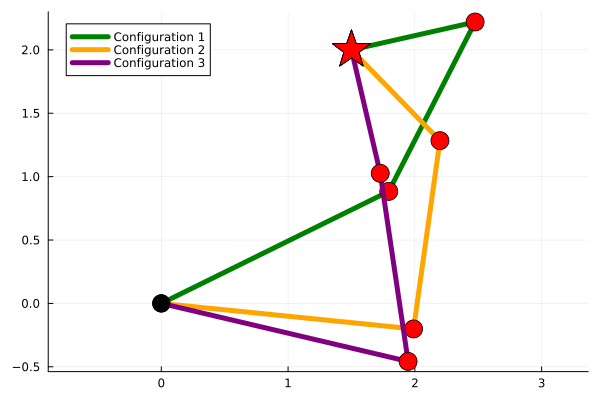
\includegraphics[width=0.6\columnwidth]{graphics/Chap06/constrainedOptimizationForRobotKinematicChain.png}%
    \caption[]{This is the same 3-link manipulator from Fig.~\ref{fig:RobotAbsoluteAngle}-(b). Here, the red star  (\textcolor{red}{\Huge $\star$}) indicates the desired position of the end of the last link, meaning it is where we are trying to position the robot's \href{https://en.wikipedia.org/wiki/Robot_end_effector}{end effector}. The precise point in Cartesian space is $p_3 = (1.5, 2)$. We see that there are numerous configurations (i.e., different values for $\theta_i$) of the robot that achieve the same position of the end effector (we only show three of an infinite number of possible configurations). Hence the problem is \textbf{underdetermined}. What is an aspiring Roboticist to do with this messy situation? \textbf{The solution is constrained minimization}.}
    \label{fig:robotKinematicsConstrainedOptimization}
\end{figure}

\bigskip

\begin{example} Sketch out a plausible argument for Proposition~\ref{thm:MultivariableSecondOrderTestLocalMaxMin}.    
\end{example}

\solution We use facts about symmetric matrices that are stated in the Appendix of the ROB 101 textbook, \textit{Computational Linear Algebra}, and proved in the ROB 501 textbook, \textit{Mathematics for Robotics}; the textbooks can be found \href{https://grizzle.robotics.umich.edu/education}{here}.  \\


Let $x^\ast \in \mathbb{R}^n$ be a critical point of $f(x)$, meaning that $\nabla f(x^\ast) = 0$. To determine the nature of stationary point, we will analyze the behavior of the second-order Taylor expansion of $f(x)$ around $x^\ast$. \\

The Hessian matrix of $f$ at $x^\ast$, denoted $H_f(x^\ast)$, is symmetric. Therefore, the eigenvalues of $H_f(x^\ast)$, denoted $\{\lambda_1, \lambda_2, \ldots, \lambda_n\}$, are real, and $H_f(x^\ast)$ has a full set of linearly independent eigenvectors, $\{ v_1, \ldots, v_n \}$. We can select these eigenvectors such that the matrix
\[
Q := \left[ v_1 ~~ v_2 ~~ \cdots ~~ v_n \right]
\]
is orthogonal, i.e., $Q^\top \cdot Q = I_n$.

\subsubsection{ Step 1: Change of Variables}

We perform a change of variables by introducing the new coordinate system $y = Q^\top (x - x^\ast)$. In this coordinate system, we will examine the Hessian and show that it is diagonal. Since $Q$ is orthogonal, this transformation preserves distances, so the nature of the critical point does not change.

\subsubsection{ Step 2: Taylor Expansion}

The second-order Taylor expansion of $f(x)$ around $x^\ast$ is:
\[
f(x) \approx f(x^\ast) + \frac{1}{2} (x - x^\ast)^\top H_f(x^\ast) (x - x^\ast).
\]
Because $\nabla f(x^\ast) = 0$, there is no first-order term. Now, using the change of variables $y = Q^\top (x - x^\ast)$, we express the quadratic form in terms of $y$:
\[
f(x) \approx f(x^\ast) + \frac{1}{2} y^\top Q^\top H_f(x^\ast) Q y
\]

\subsubsection{ Step 3: Diagonalizing the Hessian}

Because $Q$ is the matrix of eigenvectors of $H_f(x^\ast)$, we know that:
\[
Q^\top H_f(x^\ast) Q = \text{diag}(\lambda_1, \lambda_2, \ldots, \lambda_n)
\]
This is a diagonal matrix with the eigenvalues $\lambda_1, \lambda_2, \ldots, \lambda_n$ of $H_f(x^\ast)$ on the diagonal. Therefore, in the new coordinates \( y \), the second-order term becomes:
\[
f(x) \approx f(x^\ast) + \frac{1}{2} \sum_{i=1}^n \lambda_i y_i^2
\]

\subsubsection{ Step 4: Analyzing the Eigenvalues}

\begin{itemize}
    \item If all the eigenvalues $\{\lambda_1, \ldots, \lambda_n\}$ of the Hessian matrix are positive, then the quadratic form $\frac{1}{2} \sum_{i=1}^n \lambda_i y_i^2$ is strictly positive for all non-zero $y$. This implies that the function $f(x)$ is locally bowl in a neighborhood around $x^\ast$, meaning $x^\ast$ is a local minimum of $f(x)$. Similarly, if all of the eigenvalues are negative, we have the analogy of a downward pointing parabola, and hence $x^\ast$ is a local maximum.

    \item When the eigenvalues have mixed signs, such as $y_1^2 - y_2^2$ we have the classic saddle point shown in Fig.~\ref{fig:OptimizationVocabularyVisualized}. 
    
    \item When one of the eigenvalues is zero, then the test is inconclusive, just as in the scalar case.
\end{itemize}


\subsubsection{Step 5: Chain Rule Explanation}

In this proof, we used the chain rule implicitly during the change of variables. When we transformed the variable from $x$ to $y = Q^\top (x - x^\ast)$, the Hessian transforms according to the rule:
\[
H_y = Q^\top H_f(x^\ast) Q
\]
This is a standard result in Math 215 Multivariable Calculus, showing how the Hessian matrix transforms under a change of coordinates, which diagonalizes it when expressed in the eigenvector basis.

\Qed



\section{Constrained Optimization}
\label{sec:ConstrainedOptimization}

In this section, we'll first motivate the problem being addressed via a physical example. Then we cover the typical material that you would learn in Calc III for use in an engineering course. You cannot do much with it in real life, except get good grades! Hence, we'll also show you how to set up problems for that next internship and the eventual soul-satisfying, technically demanding, well-paying career. 

\subsection{Motivating Problems}

As motivation, we pose two example problems based on Fig.~\ref{fig:robotKinematicsConstrainedOptimization}. Recall that the end effector position of the robot as a function of $\theta = (\theta_1, \theta_2, \theta_3)$ was given in \eqref{eq:robotp3}. We'll first take just the $x$-component of the end effector and define the function
\begin{equation}
    g_1(\theta) :=  L1 \cdot \cos(\theta_1) + L2 \cdot \cos(\theta_1 + \theta_2) + L3 \cdot \cos(\theta_1 + \theta_2 + \theta_3) - \bm{1.5},
\end{equation}
so that $g_1(\theta) $ vanishes when the end effector is at the desired $x$-position, namely $\bm{1.5}$. Given this function, we pose, \\

\textbf{Motivating Problem 1:}
\begin{equation}
\begin{aligned}
\text{Minimize} \quad & f(\theta) := (\theta_1)^2 +  (\theta_2)^2 +  (\theta_3)^2\\
\text{subject to} \quad & g_1(\theta) = 0.
\end{aligned}    
\end{equation}
The ``\textbf{subject to}'' means that a solution to this problem is \textbf{constrained} to find values for $\theta_1$, $\theta_2$, and $\theta_3$ such that $g(\theta_1, \theta_2, \theta_3) = 0$. \textbf{Clever us designed $\bm{g_1}$ so that it only vanishes for values of $\bm{\theta}$ where the $\bm{x}$-position of the end effector is at the desired value of 1.5}. \textcolor{blue}{\bf This is why Engineers use constraints in optimization problems: we often have goals to achieve that are distinct from minimizing some quantity.}\\

\textbf{What is the role of the cost function?} Well, we already saw in Fig.~\ref{fig:robotKinematicsConstrainedOptimization} that there are an infinite number of values of $\theta_1$, $\theta_2$, and $\theta_3$ that achieve the full constraint 
$$p_3 = \left[ \begin{array}{c} 1.5 \\  2.0  \end{array} \right], $$
so there must be even more solutions that only constrain the $x$-component of $p_3$ and allows the $y$-component to be \textbf{unconstrained}. The cost function sorts through this infinite set of values and finds the one that minimizes the cost while satisfying the constraint. \textcolor{blue}{\bf This is a mainstay of modern engineering}. \\

Next, we define 
\begin{equation}
\label{eq:3LinkConstraintFull}
    g(\theta):=   \left[ \begin{array}{c} 
   g_1(\theta)\\  
    g_2(\theta)
    \end{array} \right] =
    \left[ \begin{array}{c} 
    L1 \cdot \cos(\theta_1) + L2 \cdot \cos(\theta_1 + \theta_2) + L3 \cdot \cos(\theta_1 + \theta_2 + \theta_3) -\bm{1.5}\\  
    L1 \cdot \sin(\theta_1) + L2 \cdot \sin(\theta_1 + \theta_2) + L3 \cdot \sin(\theta_1 + \theta_2 + \theta_3)  \bm{-2.0}
    \end{array} \right], 
\end{equation}
so that $g(\theta) $ vanishes when the end effector is at the desired $x$- and $y$-positions. Given this function, we pose,\\

\textbf{Motivating Problem 2:}
\begin{equation}
\label{eq:MotivatingProblem2ConstrainedOptimization}
\begin{aligned}
\text{Minimize} \quad & f(\theta) := (\theta_1)^2 +  (\theta_2)^2 +  (\theta_2)^2\\
\text{subject to} \quad & g(\theta) = 0.
\end{aligned}    
\end{equation}
You could also write the problem as 
\begin{equation}
\begin{aligned}
\text{Minimize} \quad & f(\theta) := (\theta_1)^2 +  (\theta_2)^2 +  (\theta_2)^2\\
\text{subject to} \quad & g_1(\theta) = 0 \text{ and } g_2(\theta) = 0.
\end{aligned}    
\end{equation}
Once again, the ``\textbf{subject to}'' means that a solution to this problem is \textbf{constrained} to find values for $\theta_1$, $\theta_2$, and $\theta_3$ such that $g(\theta_1, \theta_2, \theta_3) = 0$. And once again, we designed $g$ so that it only vanishes when the $(x, y)$-position of the end effector is at the desired point in Cartesian space. \textcolor{blue}{\bf We repeat: this is why Engineers use constraints in optimization problems: we have goals to achieve that are distinct from minimizing some quantity}. The cost function takes care of the ambiguity in trying to place the end effector (that depends on three angles) at the desired location (specified by a 2-vector in the plane): we have three variables and only two constraints. Hence, we have an underdetermined problem, and constrained optimization is a perfect method for resolving the ambiguity associated with undetermined problems.

\subsection{Vocabulary of Constrained Optimization}

In the context of constrained optimization, several key terms and concepts are fundamental to understanding and solving optimization problems. Below is an overview of the primary vocabulary:

\begin{itemize}
   
    \item \textbf{Cost Function}: Also known as the objective function, this is the function  $f:\real^n \to \real$ that we aim to minimize or maximize within the feasible set. The cost function quantifies the ``cost'' associated with a particular choice of \(x=(x_1, x_2, \ldots, x_n)\).

       
    \item \textbf{Decision Variables}: For a cost function, $f(x) = f(x_1, x_2, \ldots, x_n)$, the components $x_i, 1 \le i \le n$ are the decision variables. They are the variables we can search over to fin values that textremize the cost function.
    
    \item \textbf{Constraints}: Conditions that the solution \(x\) must satisfy. Constraints can be classified into two types:
    \begin{itemize}
        \item \textbf{Equality Constraints}: These require that the constraint functions equal zero, \(g(x) = 0\).
        \item \textbf{Inequality Constraints}: These specify that the constraint functions must be greater than or equal to zero, \(h(x) \geq 0\), or less than or equal to zero, depending on the problem formulation.
    \end{itemize}

        \item \textbf{Feasible Set}: The set of all points \(x\) that satisfy the constraints of the optimization problem. For equality constraints, this set includes all \(x\) such that \(g(x) = 0\), where \(g(x)\) represents the constraint functions.
    
    \item \textbf{Constraint Qualification}: A set of conditions that ensure the mathematical program has a well-defined solution. One common qualification is that the rows of the Jacobian matrix of the constraint functions \(g(x)\) are linearly independent at all points in the feasible set. Equivalently, the gradients of the constraints are linearly independent as column vectors. 
    
    \item \textbf{Lagrange Multipliers}: Numbers \(\lambda\) associated with each constraint that measure the sensitivity of the objective function's optimal value to changes in the constraint boundary. The method of Lagrange multipliers is a strategy for finding the local maxima and minima of a function subject to equality constraints.
    
    \item \textbf{KKT Conditions} (Karush-Kuhn-Tucker): Necessary conditions for a solution in nonlinear programming to be optimal, given certain regularity conditions. These conditions generalize the method of Lagrange multipliers to handle inequality constraints. (Typically covered in 400-level courses; is not treated here.)
    
    \item \textbf{Slack Variables}: Additional variables introduced to transform inequality constraints into equality constraints, making it easier to apply certain optimization methods. (Typically covered in 400-level courses; is not treated here.)
\end{itemize}

\begin{figure}[hbt]
    \centering

% TikZ code
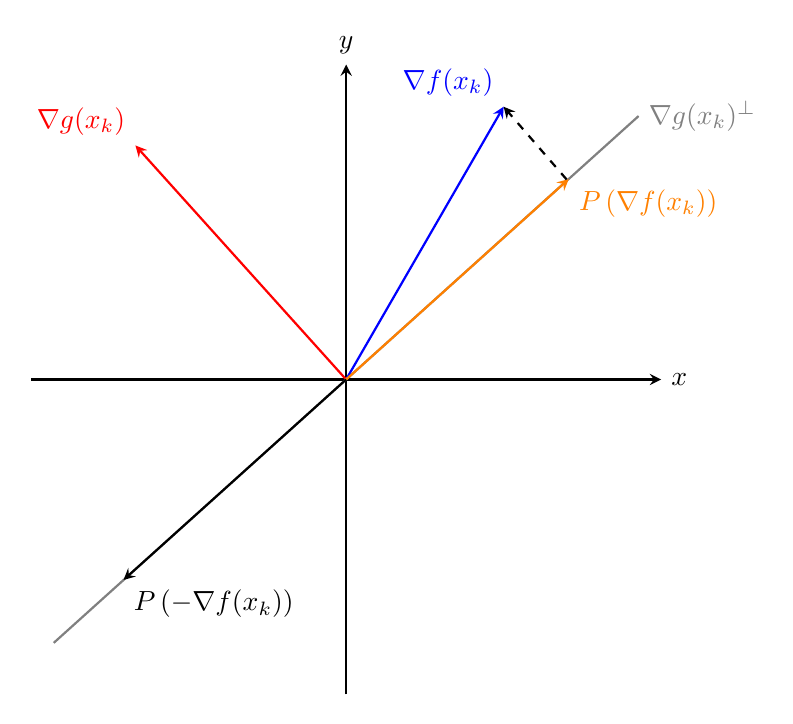
\begin{tikzpicture}[scale=2, thick, >=stealth]
    % Axes
    \draw[->] (-2,0) -- (2,0) node[right] {$x$};
    \draw[->] (0,-2) -- (0,2) node[above] {$y$};
    
    % Corrected vectors with specified angles
    \draw[->, blue] (0,0) -- (1,1.732) node[above, above left] {$\nabla f(x_k)$}; % 60 degrees CCW from x-axis
    \draw[->, red] (0,0) -- (-1.338,1.486) node[above left] {$\nabla g(x_k)$}; % 130 degrees CCW from x-axis

        % Orthogonal complement (solid line, now normal to grad g)
\draw[solid, thick, gray] (-1.857,-1.6727) -- (1.857,1.6727) node[right] {$\nabla g(x_k)^\perp$};
    


%   Projection vector
    % \draw[->, thick, purple] (0,0) -- (1.4135, 1.2727) node[midway, below right] {$P_{\nabla g(x_k)^\perp} \nabla f(x_k)$};
    \draw[->,  orange] (0,0) -- (1.4135, 1.2727) node[right, below right] {$P\left( \nabla f(x_k) \right)$};

    \draw[->,  black] (0,0) -- (-1.4135, -1.2727) node[right, below right] {$P\left( -\nabla f(x_k) \right)$};    

% Projection line (now correct)
    \draw[->, dashed] (1.4, 1.27) -- (1,1.732);  % Projection of f onto orthogonal complement of g   


\end{tikzpicture}

    \caption{Geometry of gradient descent with an equality constraint. In the image, the line labeled $\nabla g(x_k)^\perp$ is the set of points (actually, the subspace) orthogonal to $\nabla g(x_k)$, the gradient of the cost. The angle between $\nabla f(x_k)$ and $\nabla g(x_k)$ is $72^o$. The dotted line shows $\alpha \cdot \nabla g(x_k)$, the proportion of $\nabla g(x_k)$ that must be removed (aka, subtracted) from $\nabla f(x_k)$ so that $\nabla f(x_k) - \alpha \nabla g(x_k)$  is orthogonal to the constraint gradient. The new vector, denoted $P(\nabla f(x_k))$, is an ascent direction that respects the constraint, whereas $P(-\nabla f(x_k))$, is a descent direction that respects the constraint.}
    \label{fig:OthogonalProjectionGradientOnComplementGradg}
\end{figure}

\subsection{Gradient Descent with a Single Equality Constraint}

Suppose that the functions $f:\real^n \to \real$ and $g:\real^n \to \real$ define the cost and the constraint in the constrained minimization problem 
\begin{equation}
\label{eq:GenericSingleConstraintOptimizationProblemContextGradientDescent}
\begin{aligned}
\text{Minimize} \quad & f(x)\\
\text{subject to} \quad & g(x) = 0.
\end{aligned}    
\end{equation}
We seek to modify the gradient descent algorithm to accommodate the equality constraint. Let $x_k \in \real^n$  be the current value of the vector of decision variables, which we assume to be feasible, that is $g(x_k) = 0$. We seek $\Delta x$ such that
\begin{equation}
\label{eq:GradDescentConditionsForDeltax}
\begin{aligned}    
    f(x_k + \Delta x) & < f(x_k) \\
    g(x_k + \Delta x) & =0.
\end{aligned}
\end{equation}
We use our gradient notation to linearize these equations about $x_k$,
\begin{equation}
\label{eq:GradDescentLinearizedConditionsForDeltax}
\begin{aligned}    
    f(x_k + \Delta x) & \approx f(x_k)  + \nabla f(x_k) \bullet \Delta x\\
    g(x_k + \Delta x) & \approx \nabla g(x_k) \bullet \Delta x.
\end{aligned}
\end{equation}
From \eqref{eq:GradDescentConditionsForDeltax} and \eqref{eq:GradDescentLinearizedConditionsForDeltax}, we deduce that $\Delta x$ must satisfy 
\begin{equation}
\begin{aligned}    
    \nabla f(x_k) \bullet \Delta x &< 0\\
    \nabla g(x_k) \bullet \Delta x &= 0.
\end{aligned}
\end{equation}

We pose $\Delta x := -\nabla f(x_k) + \alpha \nabla g(x_k)$ and seek to choose $\alpha$ such that
$g(x_k) \bullet \Delta x = 0$. Using results from ROB 101 Computational Linear Algebra, we compute
\begin{equation}
\begin{aligned}    
    0 =& \nabla g(x_k) \bullet \Delta x \\
    \Updownarrow & \\
    0 =& \nabla g(x_k) \bullet \left( -\nabla f(x_k) + \alpha \nabla g(x_k)\right) \\
     \Updownarrow & \\
   0=& -\nabla g(x_k) \bullet \nabla f(x_k) + \alpha \nabla g(x_k) \bullet \nabla g(x_k) 
\end{aligned}
\end{equation}
Hence, if $ \nabla g(x_k) \neq 0_{n \times 1}$, then 
\begin{equation}
    \alpha = \frac{\nabla g(x_k) \bullet \nabla f(x_k)}{\nabla g(x_k) \bullet \nabla g(x_k)}
\end{equation}
and we have
\begin{equation}
    \Delta x =  - \nabla f(x_k) + \frac{\nabla g(x_k) \bullet \nabla f(x_k)}{\nabla g(x_k) \bullet \nabla g(x_k)} \cdot \nabla g(x_k).
\end{equation}
Fig~\ref{fig:OthogonalProjectionGradientOnComplementGradg} shows that this is the orthogonal projection of $-\nabla f(x_k)$ onto $\left[ \nabla g(x_k)\right]^\perp:= \{ v \in \real^n~|~ v \perp \nabla g(x_k)  \}$. In simpler terms, we have removed from $-\nabla f(x_k)$ its component lying in the direction of $\nabla g(x_k)$. This gives the basic setup for gradient descent with a single equality constraint. 
\bigskip

\begin{methodColor}{Gradient Descent with a Single Equality Constraint}{GradientDescentWithSingleEqualityConstraint} 

Consider the constrained optimization problem \eqref{eq:GenericSingleConstraintOptimizationProblemContextGradientDescent} for functions $f:\real^n \to \real$ and $g:\real^n \to \real$ with optimal value $x^\ast$. If the gradients vector $\nabla g(x^\ast) \neq 0_{n \times 1}$, then a locally optimal $x^\ast$ 
can be found as follows: \\


\textbf{Initialization:} Find a feasible point $x_0\in \real^n$, that is, a point such that $g(x_0) = 0$; this can be accomplished with \texttt{NLsolve}.

\bigskip

\textbf{Loop:} Given a point $x_k \in \real^n$, repeat the following steps to either find $x_{k+1}$ or terminate.

\begin{enumerate}
\renewcommand{\labelenumi}{(\alph{enumi})}
\setlength{\itemsep}{.2cm}

    \item \textbf{Compute:} $\nabla f(x_k)$, the gradient of $f$ at $x_k$ and $\nabla g(x_k)$, the gradient of the constraint vector. \\

 
   \item \textbf{Compute a Descent Direction that Respects the Constraint:} $ \Delta x =  - \nabla f(x_k) + \frac{\nabla g(x_k) \bullet \nabla f(x_k)}{\nabla g(x_k) \bullet \nabla g(x_k)} \cdot \nabla g(x_k)$

   \item \textbf{Update Step:} $x_{k+1}= x_k + s \cdot \Delta x$, where $s>0$ is the step size.

    \item \textbf{Termination Condition:} $||\Delta x|| < a_{\rm tol}$; in other words, no more progress can be made, and thus $x_k$ is (to numerical precision) a stationary point of the optimization problem.
\end{enumerate}


\textbf{Notes:} 
\begin{itemize}
    \item In practice, the updates $x_k$ will ``slowly'' exit the feasible set. Hence, when $|g(x_k)|$ exceeds a user-defined tolerance, a new call to \texttt{NLsolve} should be made. This is illustrated in the following code block.
    \item We'll see shortly that \textbf{\texttt{JuMP} does all of this and a whole lot more}. It is your best option for use in professional projects. Algorithms, like the one presented here, are essential for building fundamental understanding of gradient descent, the workhorse of Machine Learning (ML) and Inverse Kinematics!
\end{itemize}   
\end{methodColor}

\bigskip

\begin{figure}[htb]%
\centering
\subfloat[]{%
%\includegraphics[trim=7cm 1cm 7cm 1cm, clip, width=0.45\columnwidth]
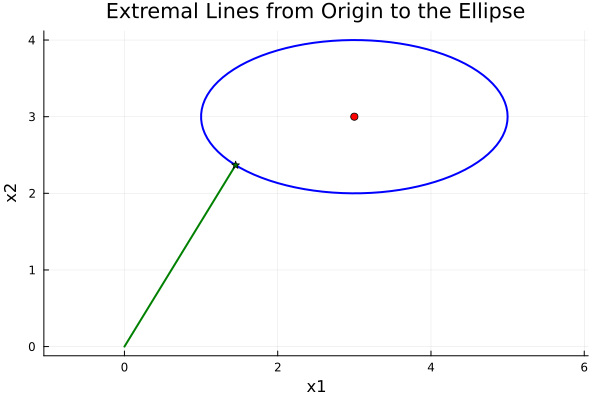
\includegraphics[width=0.45\columnwidth]{graphics/Chap06/C06_MinimumDistanceEllipse.png}
}%
%\hfill%
\hspace{.3cm}
\subfloat[]{%
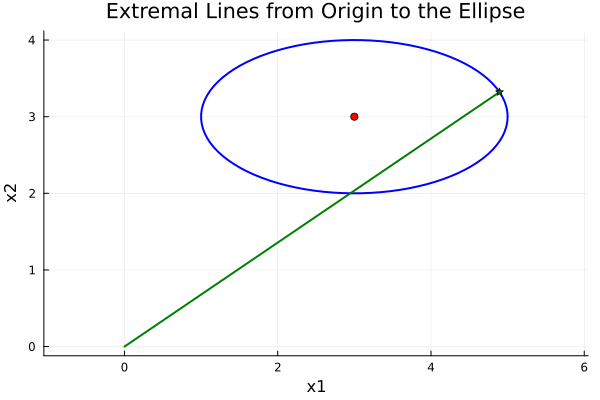
\includegraphics[ width=0.45\columnwidth]{graphics/Chap06/C06_MaximumDistanceEllipse.png}%
}
\hfill
\caption[]{Optimization with equality constraints. In these examples, the cost function is $f(x,y) = (x)^2 + (y)^2$, distance squared from the origin to $(x, y)$. The constraint is $g(x,y) = \frac{(x-x_c)^2}{a^2} + \frac{(y-y_c)^2}{b^2} - 1$, an ellipse. (a) Shows the minimum distance solution subject to $(x,y)$ lies on the ellipse, while (b) shows the maximum distance solution. The first problem uses gradient descent with one equality constraint, while the second uses gradient ascent with one equality constraint; the sign on the update step has been swapped.}
    \label{fig:GradientDescentWithOneEqualityConstraint}
\end{figure}

\bigskip

\begin{example} Solve the optimization problem \eqref{eq:GenericSingleConstraintOptimizationProblemContextGradientDescent} where the cost is $f(x,y) = x^2 + y^2$, the distance squared from the origin, and the constraint is that $(x,y)$ lies on the ellipse defined by $g(x,y)=0$, with $g(x,y) = \frac{(x-x_c)^2}{a^2} + \frac{(y-y_c)^2}{b^2} - 1$. Also find the maximizing solution. 
    
\end{example}

\solution The solution is worked out in the code block below. The results are plotted in Fig.~\ref{fig:GradientDescentWithOneEqualityConstraint}.

\Qed

\bigskip

\begin{lstlisting}[language=Julia,style=mystyle]
using ForwardDiff, LinearAlgebra, NLsolve

# Define the cost function f(x) and the equality constraints G(x)
xc = 3.0; yc = 3.0 # centers
a = 2 # x semi-major axis
b = 1.0 #y semi-major axis

# note: a = b = 1/r for a circle

# Define the cost (distance squared)
function cost(x)
    return x[1]^2 + x[2]^2
end

# Define the equality constraint: point must lie on the ellipse
function geq(x)
    # note: a = b = 1/r for a circle
    return (1/a)^2 * (x[1] - xc)^2 + (1/b)^2 * (x[2] - yc)^2 - 1
end

# Compute the gradient of the cost and constraint using ForwardDiff
grad_cost(x) = ForwardDiff.gradient(cost, x)
grad_geq(x)  = ForwardDiff.gradient(geq, x)

# Remove from the gradient of the cost any component lying along the gradient(s) of the constraint(s) 
function modGradientCost(x)
    gradCost       = grad_cost(x)
    gradConstraint = grad_geq(x)
    
    if norm(gradConstraint) < 1e-6
        println("Gradient of the constraint is essentially zero and was ignored")
        alpha = 0.0
    else
        alpha = dot(gradCost, gradConstraint) / dot(gradConstraint, gradConstraint)
    end
    
    modGradCost = gradCost - alpha * gradConstraint
    return modGradCost
end

# Function to find a feasible starting point using NLsolve
function find_feasible_point(geq, x_guess)
    # Build function for NLsolve
    function constraint!(F, x)
        F[1] = geq(x)
    end
    xFeasible = nlsolve(constraint!, x_guess)
    return xFeasible.zero
end

# Starting guess (not feasible initially)
x_guess = [0.1; 0.1]
x0 = find_feasible_point(geq, x_guess) # Make the initial guess feasible

# Set step size, max iterations, and tolerances
s = 0.1
maxIter = 1000
gradTol = 1e-6
constraintTol = 1e-4

xk = x0
for k = 1:maxIter
    modGradCost = modGradientCost(xk)  # Use the modified gradient cost function
    if norm(modGradCost) < gradTol  # Convergence check
        println("---- Iteration $k ----")
        println("Converged.")
        println("Cost: ", round.(cost(xk), digits=5))
        println("Constraints (should be near 0): ", round.(geq(xk), digits=5))
        println("----------------- ")
        break
    else
        xk = xk - s * modGradCost  # Update using the modified gradient
    end
    if norm(geq(xk)) > constraintTol
        println("Updated x to maintain g(xk)=0 at interation = $k")
        xk = find_feasible_point(geq, xk)  # Ensure feasibility
    end
end

xStar = xk
costStar = cost(xStar)
geqStar = geq(xStar)

println("\nFinal Results:")
println("-----------------")
println("Optimal x: ", round.(xStar, digits=5))
println("Optimal cost(xStar): ", round(costStar, digits=5))
println("Constraint(xStar): ", round(geqStar, digits=5))

\end{lstlisting}
\textbf{Output} 
\begin{verbatim}
Updated x to maintain g(xk)=0 at interation = 1
Updated x to maintain g(xk)=0 at interation = 2
Updated x to maintain g(xk)=0 at interation = 3
Updated x to maintain g(xk)=0 at interation = 4
Updated x to maintain g(xk)=0 at interation = 5
Updated x to maintain g(xk)=0 at interation = 6
Updated x to maintain g(xk)=0 at interation = 7
Updated x to maintain g(xk)=0 at interation = 8
---- Iteration 25 ----
Converged.
Cost: 7.70976
Constraints (should be near 0): 9.0e-5
----------------- 

Final Results:
-----------------
Optimal x: [1.45048, 2.36767]
Optimal cost(xStar): 7.70976
Constraint(xStar): 9.0e-5
\end{verbatim}

\bigskip

\subsection{Gradient Descent with a Vector of Equality Constraints}

Suppose now that in addition to the cost function $f:\real^n \to \real$, there are $m$ equality constraints, $g_i:\real^n \to \real$ in the problem
\begin{equation}
\label{eq:GenericMultiConstraintOptimizationProblemContextGradientDescent}
\begin{aligned}
\text{minimize} \quad & f(x)\\
\text{subject to} \quad & g_i(x) = 0, ~1 \le i \le m
\end{aligned}    
\end{equation}
We seek to modify the gradient descent algorithm to accommodate a vector of equality constraints. Let $x_k \in \real^n$  be the current value of the vector of decision variables, which we assume to be feasible, that is $g_i(x_k) = 0$, $1 \le i \le m$. We seek $\Delta x$ such that
\begin{equation}
\label{eq:GradDescentConditionsVector ConstraintsForDeltax}
\begin{aligned}    
    f(x_k + \Delta x) & < f(x_k) \\
    g_i(x_k + \Delta x) & =0, ~1 \le i \le m.
\end{aligned}
\end{equation}
We use our gradient notation to linearize these equations about $x_k$,
\begin{equation}
\label{eq:GradDescentLinearizedConditionsForDeltax2}
\begin{aligned}    
    f(x_k + \Delta x) & \approx f(x_k)  + \nabla f(x_k) \bullet \Delta x\\
    g_i(x_k + \Delta x) & \approx \nabla g_i(x_k) \bullet \Delta x,  ~1 \le i \le m.
\end{aligned}
\end{equation}
From \eqref{eq:GradDescentConditionsForDeltax} and \eqref{eq:GradDescentLinearizedConditionsForDeltax2}, we deduce that $\Delta x$ must satisfy 
\begin{equation}
\begin{aligned}    
    \nabla f(x_k) \bullet \Delta x &< 0\\
    \nabla g_i(x_k) \bullet \Delta x &= 0,  ~1 \le i \le m.
\end{aligned}
\end{equation}

Analogously to the single-constraint case, we pose
\begin{equation}
\label{eq:DeltaxForVectorEqualityConstraintsGradientDescent}
 \Delta x := -\nabla f(x_k) + \sum_{i=1}^m \alpha_i \nabla g_i(x_k) = -\nabla f(x_k) + \underbrace{\left[\begin{array}{cccc} \nabla g_1(x_k) & \nabla g_2(x_k)&  \cdots& \nabla g_m(x_k) \end{array} \right]}_{\nabla G(x_k)} \cdot \underbrace{\left[\begin{array}{c} \alpha_1 \\ \alpha_2 \\ \vdots \\ \alpha_m\end{array} \right] }_{\alpha}
\end{equation}
and seek to solve for $\{\alpha_1, \alpha_2, \ldots, \alpha_m\}$ such that
\begin{equation}
    \nabla g_i(x_k) \bullet \Delta x = 0, ~ 1 \le i \le m.
\end{equation}
Using results from ROB 101 Computational Linear Algebra, the above is equivalent to $\nabla G(x_k)^\top \cdot \Delta x = 0_{m \times 1}$, yielding
\begin{equation}
\label{eq:FindDeltaxGradientDescentViaLinearAlgebra}
    -\nabla G(x_k)^\top \cdot \nabla f(x_k) + \nabla G(x_k)^\top \cdot \nabla G(x_k) \cdot \alpha= 0_{m \times 1}.
\end{equation}
If the columns of $\nabla G(x_k)$ are linearly independent, then the above equation has a unique solution. For small problems, you can invert the matrix $\nabla G(x_k)^\top \cdot \nabla G(x_k)$ to solve for the vector of coefficients $\alpha$, but for larger problems, it is better to use matrix factorization, such as LU or QR. In Julia, the backslash command will choose the most appropriate method for the given problem. Also relying on ROB101, an alternative method to compute $\Delta x$ in \eqref{eq:DeltaxForVectorEqualityConstraintsGradientDescent}, is to apply Gram-Schmidt to the vectors
\begin{equation}
    \{\nabla g_1(x_k), \nabla g_2(x_k), \ldots, \nabla g_m(x_k), -\nabla f(x_k) \},
\end{equation}
where it is very important to place the gradient of the cost \textbf{after} the gradients of the constraints.

\begin{example} Define the cost by $f:\real^4 \to \real$ be $f(x_1, x_2, x_3, x_4) = \sum_{i=1}^4 (x_i)^2$, distance squared from the origin to a point $x \in \real^4$, with the constraint that $x$ must satisfy
$$0_{2 \times 1}=g(x) = \begin{bmatrix}`g_1(x) \\ g_2(x)\end{bmatrix} =  \begin{bmatrix} \frac{(x_1 - 3)^2}{2^2} + \frac{(x_2 - 3)^2}{1^2} - 1\\ x_1+x_2+x_3+x_4\end{bmatrix}.$$
This is a minimum distance problem from the origin to the feasible set, that is, $\{ x \in \real^4~|~ g(x) = 0_{2 \times 1}.$ Use gradient descent with equality constraints to solve \eqref{eq:GenericMultiConstraintOptimizationProblemContextGradientDescent}.


    
\end{example}

\solution Using Gram-Schmidt to remove the components of $\nabla g_1(x_k)$ and $\nabla g_2(x_k)$ from $\nabla f(x_k)$.


\begin{lstlisting}[language=Julia,style=mystyle]
"""
    gram_schmidt(U::Matrix)

Performs the Gram-Schmidt process on the columns of the matrix `U` (assumed to be linearly independent) 
to produce an orthogonal set of vectors stored in matrix `V` and a set of orthonormal vectors stored 
in `Vnormalized`.

# Arguments
- `U::Matrix`: A matrix whose columns are linearly independent vectors.

# Returns
- `V::Matrix`: A matrix containing the orthogonal vectors corresponding to the columns of `U`.
- `Vnormalized::Matrix`: A matrix containing the orthonormal vectors obtained by normalizing the columns of `V`.

"""

using LinearAlgebra

function gram_schmidt(U::Matrix)
    m, n = size(U)  # m = number of rows, n = number of columns (vectors)
    V = Matrix{Float64}(undef, m, n)  # Matrix to store orthogonal vectors
    Vnormalized = Matrix{Float64}(undef, m, n)  # Matrix to store normalized orthogonal vectors
    
    for i in 1:n
        # Start with the original vector from U
        vi = U[:, i]
        
        # Subtract projections onto previous vectors
        for j in 1:i-1
            vj = V[:, j]
            vi -= (dot(vi, vj) / dot(vj, vj)) * vj
        end
        
        # Store the orthogonal vector
        V[:, i] = vi
        
        # Normalize the vector and store in Vnormalized
        Vnormalized[:, i] = vi / norm(vi)
    end
    
    return (V=V, Vnormalized=Vnormalized)
end
\end{lstlisting}
\textbf{Output} 
\begin{verbatim}
gram_schmidt (generic function with 1 method)
\end{verbatim}

\begin{lstlisting}[language=Julia,style=mystyle]
# Example gradient descent with several equality constraints
# Not in the textbook

using ForwardDiff, LinearAlgebra, NLsolve, Random

# Set the seed to a specific value, for example, 1234
Random.seed!(1234)



# Define the cost function f(x) and the equality constraint G(x)
xc = 3.0; yc = 3.0 # centers
a = 2.0 # x semi-major axis
b = 1.0 # y semi-major axis

# Define the cost (distance squared)
function cost(x)
    return x[1]^2 + x[2]^2 + x[3]^2 + x[4]^2
end

# Define the equality constraint: point must lie on the ellipse
function Geq(x)
    # Equality constraints evaluated at x
    g1 = (1/a)^2 * (x[1] - xc)^2 + (1/b)^2 * (x[2] - yc)^2 - 1 # ellipse in R4
    g2 = x[1] + x[2] + x[3] + x[4] # 3 dimensional plane through the origin
    return [g1, g2]  # Return evaluated constraints as an array
end

# Compute the gradient of the cost and constraint using ForwardDiff
grad_cost(x) = ForwardDiff.gradient(cost, x)
Jac_constraints(x) = ForwardDiff.jacobian(Geq, x)

# Remove the component of the gradient of the cost lying along the gradient of the constraints
function modNegGradientCost(x)
    gradCost = grad_cost(x)
    matGradientsConstraints = Jac_constraints(x)' # transpose of Jacobian for constraint gradients
    
    # Perform Gram-Schmidt on constraint gradients and cost gradient
    U = [matGradientsConstraints gradCost]
    F = gram_schmidt(U)
    modNegGradCost = -F.V[:,end] #it's the negative of the last vector in the matrix when doing Gradient Descent 
    return modNegGradCost
end

# Function to find a feasible starting point using NLsolve
function find_feasible_point(Geq, x_guess)
    function constraint!(F, x)
        F[1] = Geq(x)[1]
        F[2] = Geq(x)[2]
    end
    result = nlsolve(constraint!, x_guess)
    return result.zero
end

# Set step size, max iterations, and tolerances
s = 0.1
maxIter = 1000
gradTol = 1e-6
constraintTol = 1e-5

# Starting guess (not feasible initially)
x_guess = rand(4,1)
xk = find_feasible_point(Geq, x_guess) # Make the initial guess feasible

# Gradient Descent with equality constraints loop
for k = 1:maxIter
    modNegGradCost = modNegGradientCost(xk)  # Use the modified gradient cost function
    if norm(modNegGradCost) < gradTol  # Convergence check
        println("\n---- Iteration $k ----")
        println("Converged.")
        println("Cost: ", round.(cost(xk), digits=5))
        println("Constraints (should be near 0): ", round.(Geq(xk), digits=6))
        println("----------------- ")
        break
    else
        xk = xk + s * modNegGradCost  # Update using the modified gradient
    end
    
    if norm(Geq(xk)) > constraintTol  # Feasibility check
        println("Updating for feasibility: G(xk) = 0_{m x 1} at iteration k = $k")
        xk = find_feasible_point(Geq, xk)  # Ensure feasibility
    end
end

# Final results
xStar = xk
costStar = cost(xStar)

println("\nFinal Results:")
println("-----------------")
println("Optimal x: ", round.(xStar, digits=5))
println("Optimal cost(xStar): ", round(costStar, digits=5))
println("Minimal Distance is sqrt(cost(xStar)): ", round(sqrt(costStar), digits=5))
\end{lstlisting}
\textbf{Output} 
\begin{verbatim}
Updating for feasibility: G(xk) = 0_{m x 1} at iteration k = 1
Updating for feasibility: G(xk) = 0_{m x 1} at iteration k = 2

---- Iteration 63 ----
Converged.
Cost: 14.91277
Constraints (should be near 0): [0.0, -0.0]
----------------- 

Final Results:
-----------------
Optimal x: [1.33912; 2.44289; -1.89101; -1.89101;;]
Optimal cost(xStar): 14.91277
Minimal Distance is sqrt(cost(xStar)): 3.86171

\end{verbatim}

\solution This time using \eqref{eq:FindDeltaxGradientDescentViaLinearAlgebra} to update $\Delta x$.

\begin{lstlisting}[language=Julia,style=mystyle]
# Example gradient descent with several equality constraints
# Not in the textbook

using ForwardDiff, LinearAlgebra, NLsolve, Random

# Set the seed to a specific value, for example, 1234
Random.seed!(1234)



# Define the cost function f(x) and the equality constraint G(x)
xc = 3.0; yc = 3.0 # centers
a = 2.0 # x semi-major axis
b = 1.0 # y semi-major axis

# Define the cost (distance squared)
function cost(x)
    return x[1]^2 + x[2]^2 + x[3]^2 + x[4]^2
end

# Define the equality constraint: point must lie on the ellipse
function Geq(x)
    # Equality constraints evaluated at x
    g1 = (1/a)^2 * (x[1] - xc)^2 + (1/b)^2 * (x[2] - yc)^2 - 1 # ellipse in R4
    g2 = x[1] + x[2] + x[3] + x[4] # 3 dimensional plane through the origin
    return [g1, g2]  # Return evaluated constraints as an array
end

# Compute the gradient of the cost and constraint using ForwardDiff
grad_cost(x) = ForwardDiff.gradient(cost, x)
Jac_constraints(x) = ForwardDiff.jacobian(Geq, x)

# Remove the component of the gradient of the cost lying along the gradient of the constraints
function modNegGradientCost(x)
    gradCost = grad_cost(x)
    matGradientsConstraints = Jac_constraints(x)' # transpose of Jacobian for constraint gradients
    
    alpha = (matGradientsConstraints)'*matGradientsConstraints \ matGradientsConstraints'*gradCost
    
    modNegGradCost = -gradCost + matGradientsConstraints *alpha #it's the negative of the last vector in the matrix when doing Gradient Descent 
    return modNegGradCost
end

# Function to find a feasible starting point using NLsolve
function find_feasible_point(Geq, x_guess)
    function constraint!(F, x)
        F[1] = Geq(x)[1]
        F[2] = Geq(x)[2]
    end
    result = nlsolve(constraint!, x_guess)
    return result.zero
end

# Set step size, max iterations, and tolerances
s = 0.1
maxIter = 1000
gradTol = 1e-6
constraintTol = 1e-5

# Starting guess (not feasible initially)
x_guess = rand(4,1)
xk = find_feasible_point(Geq, x_guess) # Make the initial guess feasible

# Gradient Descent with equality constraints loop
for k = 1:maxIter
    modNegGradCost = modNegGradientCost(xk)  # Use the modified gradient cost function
    if norm(modNegGradCost) < gradTol  # Convergence check
        println("\n---- Iteration $k ----")
        println("Converged.")
        println("Cost: ", round.(cost(xk), digits=5))
        println("Constraints (should be near 0): ", round.(Geq(xk), digits=6))
        println("----------------- ")
        break
    else
        xk = xk + s * modNegGradCost  # Update using the modified gradient
    end
    
    if norm(Geq(xk)) > constraintTol  # Feasibility check
        println("Updating for feasibility: G(xk) = 0_{m x 1} at iteration k = $k")
        xk = find_feasible_point(Geq, xk)  # Ensure feasibility
    end
end

# Final results
xStar = xk
costStar = cost(xStar)

println("\nFinal Results:")
println("-----------------")
println("Optimal x: ", round.(xStar, digits=5))
println("Optimal cost(xStar): ", round(costStar, digits=5))
println("Minimal Distance is sqrt(cost(xStar)): ", round(sqrt(costStar), digits=5))

\end{lstlisting}
\textbf{Output} 
\begin{verbatim}
Updating for feasibility: G(xk) = 0_{m x 1} at iteration k = 1
Updating for feasibility: G(xk) = 0_{m x 1} at iteration k = 2

---- Iteration 63 ----
Converged.
Cost: 14.91277
Constraints (should be near 0): [0.0, -0.0]
----------------- 

Final Results:
-----------------
Optimal x: [1.33912; 2.44289; -1.89101; -1.89101;;]
Optimal cost(xStar): 14.91277
Minimal Distance is sqrt(cost(xStar)): 3.86171
\end{verbatim}

% \begin{lstlisting}[language=Julia,style=mystyle]

% \end{lstlisting}
% \textbf{Output} 
% \begin{verbatim}

% \end{verbatim}



\subsection{Lagrange Multiplier for a Problem with a Single Equality Constraint}

The method of Lagrange multipliers is a tool that reduces optimization problems subject to equality constraints to what looks like an unconstrained problem. The new problem has dimension $(n+1)$ instead of $n$, but at least you can apply the methods of Chapter~\ref{sec:MinNoConstraints} to solve it. Mathematicians are very good at taking what looks like a new, super-hard problem and reducing its solution to a problem they already know how to solve. It's a power mindset! Engineers have learned to do this, too, by the way.

\begin{propColor}{Lagrange Multiplier Theorem for Constrained Optimization}{LagrangeMultipliers}

Suppose that the functions $f:\real^n \to \real$ and $g:\real^n \to \real$ define the cost and the constraint in the constrained minimization problem 
\begin{equation}
\label{eq:GenericSingleConstraintOptimizationProblem}
\begin{aligned}
\text{Minimize} \quad & f(x)\\
\text{subject to} \quad & g(x) = 0.
\end{aligned}    
\end{equation}
If $x^\ast$ is a solution to \eqref{eq:GenericSingleConstraintOptimizationProblem} \textbf{and} $\frac{\partial g(x^\ast)}{\partial x} \neq 0$, then there exists a unique scalar $\lambda^\ast \in \real$ such that
\begin{equation}
\label{eq:EquivalentUnconstrainedOptimizationProblem01}
\nabla f(x^\ast) + \lambda^\ast \nabla g(x^\ast) = 0,
\end{equation}
in other words, $x^\ast$ is a \textbf{stationary point of the unconstrained (cost) function}
$$ L(x, \lambda^*):= f(x) = \lambda^\ast g(x).$$
% Because the gradient of a scalar-valued function is the transpose of its Jacobian, the condition \eqref{eq:EquivalentUnconstrainedOptimizationProblem01} is equivalent to 
% \begin{equation}
% \label{eq:EquivalentUnconstrainedOptimizationProblem02}
% \nabla f(x^\ast) + \lambda^\ast \nabla g(x^\ast) = 0.
% \end{equation}

\begin{rem}
For reasons we will see shortly, 
\begin{enumerate}
\renewcommand{\labelenumi}{(\alph{enumi})}
\setlength{\itemsep}{.2cm}

\item the constant $\lambda^\ast$ is called the \textbf{Lagrange Multiplier} associated with the constrained minimization problem, \eqref{eq:GenericSingleConstraintOptimizationProblem}, and 

\item $L(x, \lambda): f(x) + \lambda g(x)$ (with a general $\lambda$ instead of a specific value) is the \textbf{Lagrangian} associated with \eqref{eq:GenericSingleConstraintOptimizationProblem}.

\item So far, we have not told you how to find the Lagrange multiplier; that is done in Method~\ref{thm:MethodLagrangeMultipliers}. But at least you understand why it is important: it reduces a problem we do not know how to solve to one we do know how to solve.

\item Because maximizing a function is the same as minimizing its negative, all of the above holds for constrained maximization problems as well. In fact, if you succeed in computing all of the stationary points of $L$, you will have found all of the minima of $f$, all of the maxima of $f$, and its saddle points. The stationary conditions are agnostic to min versus max. 

\item A similar result can be given when there are several constraints, as in our Motivating Problem 2 in \eqref{eq:MotivatingProblem2ConstrainedOptimization}. The multi-constraint result will be placed in an ``Optional Read'' section along with an algebraic proof of the Method of Lagrange Multipliers, based on knowledge from ROB 101 \textit{Computational Linear Algebra}. 
\end{enumerate}
    
\end{rem}    
\end{propColor}

\bigskip

\begin{methodColor}{Method of Lagrange Multipliers}{MethodLagrangeMultipliers} Consider the constrained optimization problem \eqref{eq:GenericSingleConstraintOptimizationProblem} for functions $f:\real^n \to \real$ and $g:\real^n \to \real$ with optimal value $x^\ast$. If $\frac{ \partial g(x^\ast)}{\partial x} \neq 0$, then the optimal $x^\ast$ \textbf{and} $\lambda^\ast$ can be found as follows: \\

\textbf{Step 1:} Form the \textbf{Lagrangian} function
\begin{equation}
    L(x, \lambda):= f(x) + \lambda g(x).
\end{equation}

\bigskip

\textbf{Step 2:} Solve for the \textbf{stationary points}\footnote{A nice discussion on this aspect of Lagrange's Method is given in \href{https://tinyurl.com/bde7vtbp}{Example 5: Numerical optimization} of Wikipedia.} of $L$, that is, find all solutions to
\begin{equation}
\label{eq:LagrangeStationaryConditionsGradForm}
0_{(n+1)\times 1} = \nabla L(x, \lambda).
\end{equation}
When the compact notation in \eqref{eq:LagrangeStationaryConditionsGradForm} is expanded out,  the terms needed in a calculation become more evident, namely
\begin{equation}
\label{eq:LagrangeStationaryConditions}
\begin{aligned}
     0_{n \times 1} & = \left[ \begin{array}{c}
         \frac{L(x, \lambda)}{\partial x_1} \medskip \\
          \frac{L(x, \lambda)}{\partial x_2} \medskip \\
          \vdots \\
           \frac{L(x, \lambda)}{\partial x_n}
    \end{array}\right]
 = \nabla f(x) + \lambda \nabla g(x) \medskip \\
     0_{1 \times 1} & = \frac{ \partial L(x, \lambda)}{\partial \lambda} = g(x).
\end{aligned}
\end{equation}
For small problems, the calculations are easy to do by hand. For ``smallish to medium-sized problems'', the \texttt{Symbolics} package makes short work of computing the gradient of $L$, and \texttt{NLSolve} can be ``coaxed'' into finding the roots of the gradient, that is, the stationary points.\\

The notation, $0_{1 \times 1}$, instead of $0$, emphasizes that this line is scalar-valued; in fact, it imposes the scalar-valued (feasibility) constraint, $g(x) = 0$. We note that \eqref{eq:LagrangeStationaryConditions} has $(n+1)$ equations in $(n+1)$ unknowns, $(x, \lambda)$, which is why we \textbf{can now solve} for the Lagrange multiplier $\lambda^\ast$, in addition to $x^\ast$.\\

\textbf{Step 3:} Evaluate the cost function $f(x)$ at each of the stationary points and choose the one (or ones) yielding a minimum. At this stage, we no longer have to worry about the constraint, $g(x)$, because it was taken care of in the computation of the stationary points of the Lagrangian, $L$.  

\end{methodColor}

\bigskip

We next solve a few examples that are on the level of difficulty that you will find in your 200- and 300-level Engineering courses. \textbf{With the exception of Robotics and IOE, the problems must be solvable algebraically because you will not be assumed to know anything about numerical methods}. You will have to solve them by hand, with paper and pencil.

\begin{figure}[ht]
    \centering
    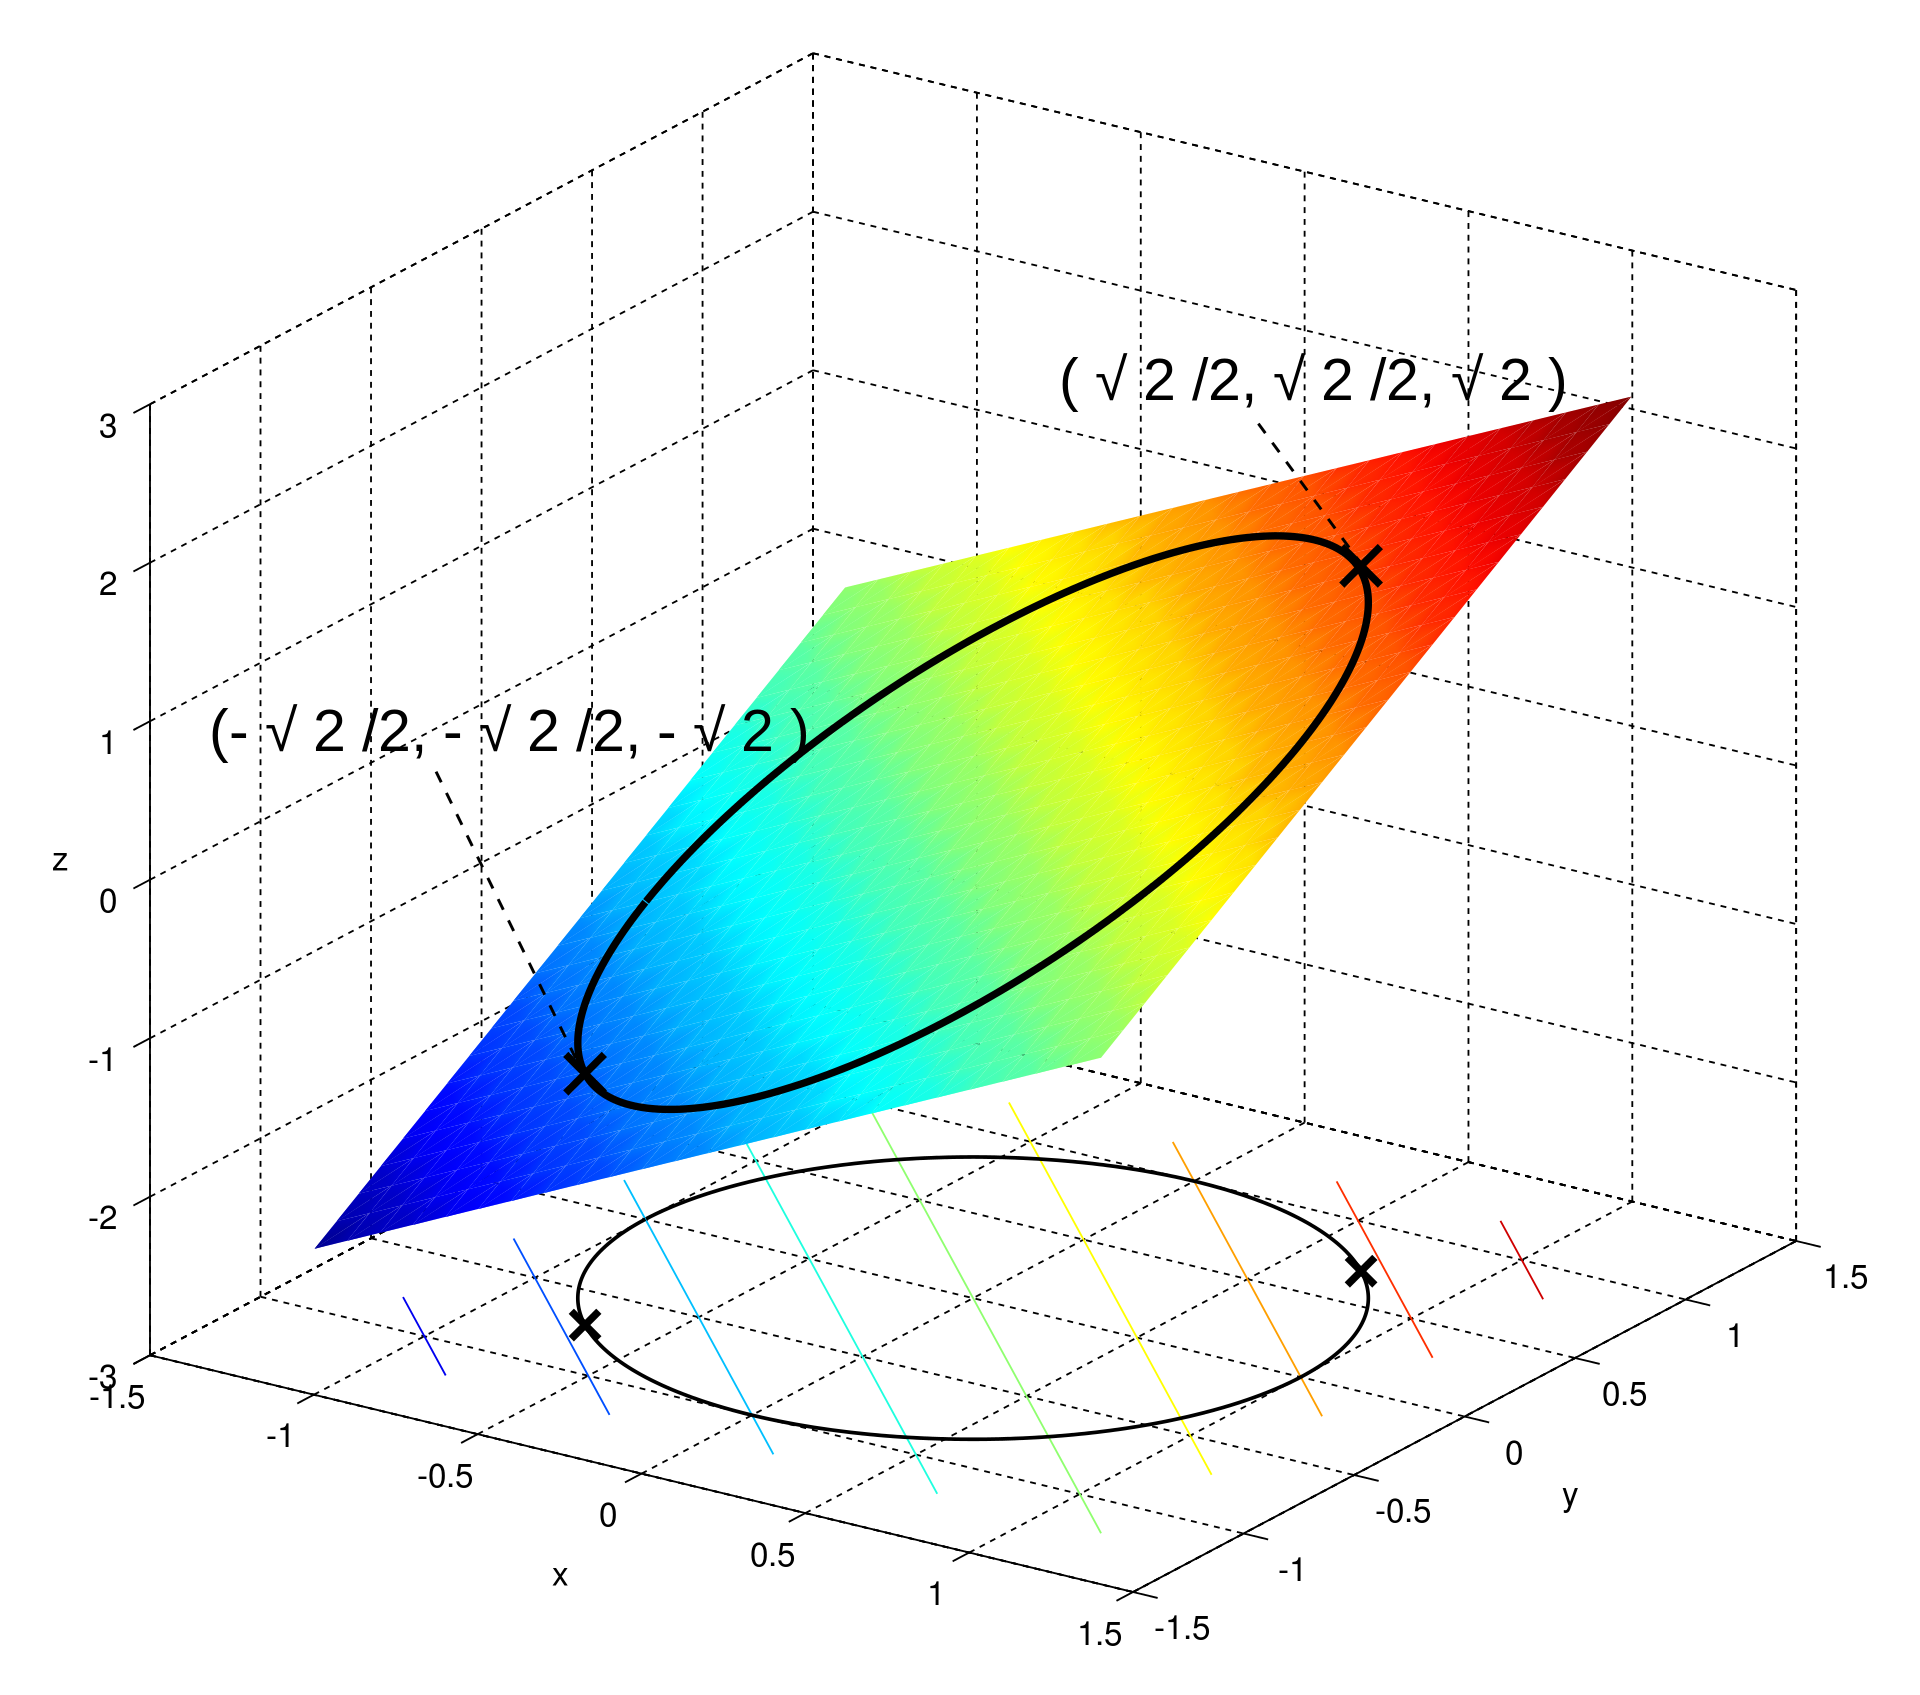
\includegraphics[width=0.7\columnwidth]{graphics/Chap06/Lagrange_very_simple.svg.png}
    \caption{Illustration of a simple constrained optimization problem. For those who prefer geometric reasoning, the lines shown in the $(x,y)$-plane are the contour lines of the cost function, that is, lines along which $z = f(x, y)= x + y$ is constant. The unit circle is the constraint set, $g(x, y) = x^2 + y^2 - 1 = 0$. Hence, the set of feasible points is the unit circle. {\bf Image Credit:} \href{https://en.wikipedia.org/wiki/Lagrange\_multiplier\#\~:text=\%5Bedit\%5D-,Example\%201,-\%5Bedit\%5D}{Wikipedia: Lagrange Multipliers: Example 1}.}
    \label{ig:SimpleLagrangeMultiplier}
\end{figure}

\begin{example} 
\label{ex:lagrangeMultiplierExample01}
Use the Method of Lagrange Multipliers to minimize \( x+y \) subject to the constraint \( x^2 + y^2 = 1 \).  Note that the problem is employing standard ``non-vector'' notation where one uses $(x, y)$ to denote a point in $\real^2$ instead of $x = (x_1, x_2)^\top$.  \\

The Example is based on \href{https://en.wikipedia.org/wiki/Lagrange_multiplier#:~:text=%5Bedit%5D-,Example%201,-%5Bedit%5D}{Wikipedia, Example 1}. You may also want to look at \href{https://en.wikipedia.org/wiki/Lagrange_multiplier#:~:text=%5Bedit%5D-,Example%201,-%5Bedit%5D}{Wikipedia, Example 2}, which we will not work.
\end{example}

\textbf{Solution:} Though it is not required, we write down the constrained optimization problem,
\begin{align*}
\text{Minimize} \quad & f(x,y)=x+y\\
\text{subject to} \quad & 0 = g(x,y) = x^2 + y^2 -1,
\end{align*}
so as to make the identification of $f:\real^2 \to \real$ and $g:\real^2 \to \real$ crystal clear. Following the steps of Method~\ref{thm:MethodLagrangeMultipliers}, we define
$$L(x,y, \lambda):=(x + y) + \lambda \left(x^2 + y^2 -1\right).$$
We then compute the required partial derivatives
\begin{equation}
\label{eq:LagrangeStationaryConditionsExample1}
\begin{aligned}
0 &= \frac{ \partial L(x, y, \lambda)}{\partial x} = 1 + 2  \lambda \cdot x \\
0 &= \frac{ \partial L(x, y, \lambda)}{\partial y} = 1 + 2 \lambda \cdot y \\
0 &= \frac{ \partial L(x, y, \lambda)}{\partial \lambda} = x^2 + y^2 -1.    
\end{aligned}
\end{equation}
Note that the first two lines of the above equation correspond to the first $2 \times 1$ block of \eqref{eq:LagrangeStationaryConditions}, and the last line of the above equation corresponds to the last line of \eqref{eq:LagrangeStationaryConditions}. \\

Fortunately for us --\textbf{and it has to be like this for the problem to be doable by hand}-- we can easily solve the stationary conditions in \eqref{eq:LagrangeStationaryConditionsExample1} for $x$ and $y$ in terms of $\lambda$, giving us
\begin{align*}
    x &= - \frac{1}{2 \lambda} \\
    y &= - \frac{1}{2 \lambda}.
\end{align*}
Plugging these values into the constraint yields
$$0=-1 + x^2 + y^2 = -1 + \left(  - \frac{1}{2 \lambda}\right)^2  + \left(  - \frac{1}{2 \lambda}\right)^2 = -1 + \frac{1}{2} \frac{1}{\lambda^2},$$
or
$$\lambda^2 = \frac{1}{2}, $$
and therefore, $\lambda = \pm \frac{1}{\sqrt{2}} = \pm \frac{\sqrt{2}}{2}$. Putting all of this together and doing the messy, mistake-prone algebra, yields the hand-computed stationary points of the Lagrangian are
$$\left[\begin{array}{c}
x^\ast\\
y^\ast\\
\lambda^\ast \\
\end{array} \right] = \left[\begin{array}{r}
\frac{\sqrt{2}}{2}\\
\frac{\sqrt{2}}{2}\\
-\frac{\sqrt{2}}{2} \\
\end{array} \right] \text{ and } \left[\begin{array}{c}
x^\ast\\
y^\ast \\
\lambda^\ast \\
\end{array} \right] = \left[\begin{array}{r}
-\frac{\sqrt{2}}{2}\\
-\frac{\sqrt{2}}{2}\\
\frac{\sqrt{2}}{2} \\
\end{array} \right].$$
As promised, we have found $\lambda^\ast$! (Exclamation point, and not factorial.)\\

Evaluating the cost function \( f(x,y) = x+y \) at these points yields
$$f\left(\frac{\sqrt{2}}{2}, \frac{\sqrt{2}}{2}\right) = \sqrt{2}, \text{ and }  f\left(-\frac{\sqrt{2}}{2}, -\frac{\sqrt{2}}{2} \right) = -\sqrt{2}. $$
Thus the constrained minimum is \( -\sqrt{2} \), and if we had wanted it, the constrained maximum is \( \sqrt{2} \).
\Qed. 

\bigskip 

\begin{example}  Let's check that Prop.~\ref{thm:LagrangeMultipliers} really does work by re-solving Example~\ref{ex:lagrangeMultiplierExample01} with the side information that 
$$ \lambda^\ast = \frac{\sqrt{2}}{2}.$$
The goal is to check that we can find the minimum to the constrained problem by computing the stationary points of the unconstrained problem
$$ L^\ast(x, y):= L(x, y, \lambda^\ast) = x+y  + \underbrace{\frac{\sqrt{2}}{2}}_{\lambda^\ast}  \left(x^2 + y^2 -1  \right). $$ 
\end{example}

\textbf{Solution:} We compute the gradient of $L^\ast$ and set it equal to zero, namely
$$
       0_{2 \times 1} =  \nabla L^\ast(x, y) = \left[\begin{array}{c}
\frac{\partial  L^\ast(x, y)}{\partial x}\\
\frac{\partial  L^\ast(x, y)}{\partial y}
\end{array} \right] =
\left[\begin{array}{c}
1 + \sqrt{2} x \\
1 + \sqrt{2} y 
\end{array} \right].
$$
Solving for $x$ and $y$ gives the same answer we computed in Example~\ref{ex:lagrangeMultiplierExample01}, once we simplify via $\frac{1}{\sqrt{2}} = \frac{\sqrt{2}}{2}$.\\

\textbf{Notes:}
\begin{itemize}
    \item If we had wanted to find the maximum via the unconstrainted problem, we would have used $\lambda^\ast = -\frac{\sqrt{2}}{2}$.
    \item All of this is just a theoretical exercise to underline that Lagrange's Method is intimately tied to the gradient of an appropriately defined cost function. If you don't get it, just realize that no 200- or 300-level Engineering course will test you on the theoretical underpinnings of Lagrange's Method. And if it is broached in a 400-level course, it will be taught (again) in the course. Second time is charm! 
\end{itemize}

\Qed

\bigskip


\textcolor{blue}{\bf This next problem is a Calc III Classic: Minimize the surface area of a cylindrical can, subject to a constraint on its volume}. Why minimize surface area? Because that accounts for the amount of material it takes to manufacture the can, that is, its cost. Why constrain volume? To sell you a fixed amount of stuff. To formulate this problem, we need to recall two facts from High School Geometry:
\begin{itemize}
    \item Volume of a \href{https://byjus.com/maths/right-circular-cylinder/}{right circular cylinder} of height $h>0$ and radius $r>0$ is $V(r, h) = \pi \cdot r^2 \cdot h$.
    \item Surface area of the same cylinder is $S(r, h) = \underbrace{2 \pi \cdot r \cdot h}_{\text{side of cylinder}} + \underbrace{2 \pi \cdot r^2}_{\text{area of ends}} = 2 \pi \cdot (r \cdot h + r^2)$.
\end{itemize}
Yes, we are writing them as functions. And yes, a can has two ends! If you want to know more about the cost of manufacturing tin cans, see \href{https://www.procurementresource.com/production-cost-report-store/tin-can}{Tin Can Production Cost Reports}. 

\bigskip
\begin{example} Minimize the surface area of a cylindrical can of radius $r$ and height $h$ subject to its volume being equal to $V_0$.    
\end{example}

\textbf{Solution:} Though it is not required, we write down the constrained optimization problem,
\begin{align*}
\text{Minimize} \quad & f(r,h)=S(r,h) = 2 \pi \cdot (r \cdot h + r^2)\\
\text{subject to} \quad & 0 = g(r,h) = V(r,h)-V_0 = 2 \pi \cdot r^2 \cdot h - V_0,
\end{align*}
so as to make the identification of $f:\real^2 \to \real$ and $g:\real^2 \to \real$ crystal clear. Following the steps of Method~\ref{thm:MethodLagrangeMultipliers}, we define
$$L(r,h, \lambda):=2 \pi \cdot (r \cdot h + r^2) + \lambda \left(  2 \pi \cdot r^2 \cdot h - V_0\right).$$
We then compute the required partial derivatives 
\begin{equation}
\label{eq:LagrangeStationaryConditionsExample2}
\begin{aligned}
0 &= \frac{ \partial L(r, h, \lambda)}{\partial r} =  2 \pi \cdot \left( h + 2  r \right) +4 \pi \cdot \lambda \cdot r \cdot h   =
2 \pi \cdot \left( h + 2  r  + 2 \lambda \cdot r \cdot h \right) \\
0 &= \frac{ \partial L(r, h, \lambda)}{\partial h} =  2 \pi \cdot r + 2  \pi \lambda \cdot  r^2 =
2 \pi \cdot r \cdot ( 1 + \lambda \cdot r)\\
0 &= \frac{ \partial L(r, h, \lambda)}{\partial \lambda} = 2 \pi \cdot r^2 \cdot h - V_0.    
\end{aligned}
% 2 \pi \cdot r + = 2 \pi \cdot r \cdot \left( 1 + \lambda\right) 
\end{equation}
Again, note that the first two lines of the above equation correspond to the first $2 \times 1$ block of \eqref{eq:LagrangeStationaryConditions}, and the last line of the above equation corresponds to the last line of \eqref{eq:LagrangeStationaryConditions}. \\

Fortunately for us --\textbf{and it has to be like this for the problem to be doable by hand}-- we can solve for $r$, $h$ and $\lambda$ using elementary algebraic manipulations. Indeed, from the second stationary condition, if $r \neq 0$, which is required for a physical can to have a non-zero volume, we obtain 
$$
\lambda \cdot r = -1. 
$$
Plugging this value into the first  stationary condition, we obtain 
$$(0= h + 2r - 2 h ) \iff  (h = 2r).$$
Plugging this into the last stationary condition, that is, the constraint, yields
$$\left(  0 =  2 \pi \cdot r^2 \cdot (2 r) - V_0\right) \iff V_0 = 4 \pi \cdot r^3.$$
Hence, 
\begin{align*}
    r & = \sqrt[3]{\frac{V_0}{4 \pi}} \\
    h & = 2 \cdot \sqrt[3]{\frac{V_0}{4 \pi}}.
\end{align*}
We could stop here. However, just to be super complete, putting all of this together after using 
 $$( \lambda \cdot r = -1)  \iff \left(\lambda = - \frac{1}{r}\right),$$
 we obtain
$$\left[\begin{array}{c}
r^\ast\\
h ^\ast\\
\lambda^\ast \\
\end{array} \right] = \left[\begin{array}{r}
\sqrt[3]{\frac{V_0}{4 \pi}} \medskip \\
2 \cdot \sqrt[3]{\frac{V_0}{4 \pi}} \medskip \\
 - ~\sqrt[3]{\frac{4 \pi}{V_0}}\\
\end{array} \right] .$$
As promised, by using Lagrange's Method, we have found $\lambda^\ast$ as well as the proper dimensions of the can. Does someone have a patent on this? We mean the can's dimensions. Who's going to buy a Lagrange Multiplier? Maybe L'H\^opital? \\

In this case, we only found one extremal solution, the minimizing solution. You might ask yourself, why? \textbf{Why can't you maximize the surface area of a tin can?} Well, theoretically, you can do it. If we go back to our second stationary condition,
$$0 = \frac{ \partial L(r, h, \lambda)}{\partial h}= 2 \pi \cdot r \cdot ( 1 + \lambda \cdot r),$$
there was a second solution, namely, $r = 0$. Well, replacing that with $r = \epsilon>0$ and solving for $h$ such that 
$V_0 = 2 \pi \cdot r^2 \cdot h$ gives 
$$ h = \frac{V_0}{2 \pi \epsilon^2}.$$
Now, take the limit as $\epsilon \to 0^{+}$ and you get a ``can'' that is infinitely tall and narrow with a fixed volume. What is its surface area?
$$ S =2 \pi \cdot (r \cdot h + r^2) = 2 \pi \cdot (\epsilon  \cdot \frac{V_0}{2 \pi \epsilon^2} + \epsilon^2) = 2 \pi \cdot (\frac{V_0}{2 \pi \epsilon} + \epsilon^2) \to \infty \text{ as } \epsilon \to 0^+.$$
 \textbf{Hence, if you pose the nonsensical question of maximizing the surface area subject to a fixed volume, you can compute the nonsensical answer, as long as you believe in limits!} To be clear, if you give this sort of problem to a numerical solver, it will go nuts. 
\Qed. 
\\

If you enjoy the idea of objects that have strange properties, such as finite volume and infinite surface area, you may enjoy the video \href{https://www.youtube.com/watch?v=yZOi9HH5ueU}{Gabriel's Horn Paradox} by Numberphile (aka, The  \textbf{Painter's Paradox}) or \href{https://youtu.be/p-LbzWmm2zk}{Torricelli's 2nd Paradox and its 14th-century genius monk resolution} by Mathologer. The volume of the horn is finite, it is built from infinitely thin material so that the surface areas inside and outside the horn are the same, has a finite ``bell'' or ``flare'' at one end (instead of our uniformly thin cylinder), and yet it cannot be painted with a finite volume of paint. What's the paradox? Well, you can fill the horn with a finite volume of paint, and that volume is touching the inner surface of the horn, isn't it? Don't let this hurt your brain too much: this is a souped-up version of maximizing the surface area of a cylinder subject to a fixed volume. 

% YouTube is full of math videos that are click-bait for hurting your brain with some twisted ``paradox'', or something pointless like, \href{https://www.youtube.com/watch?v=7_PST7gwXRw}{90\% Fail to Solve this Correctly!} Who cares? PEMDAS be ``darned''; it's always good to throw in extra parentheses to avoid confusion.

% \jwg{Ask a GSI or IA to solve: Maximize the volume of a cylindrical can, subject to a constraint on its surface area using the \texttt{Symbolic} package in Julia. Or add it to HW??? }

% This next problem is a Calc III Classic: Maximize the volume of a cylindrical can, subject to a constraint on its surface area. Why a constraint on surface area? Because that accounts for the amount of material it takes to manufacture the can, that is, its cost. Why maximize volume? To sell you more stuff. To formulate this problem, we need to recall two facts from High School Geometry:
% \begin{itemize}
%     \item Volume of a cylinder of height $h>0$ and radius $r>0$ is $V(r, h) = \pi \cdot r^2 \cdot h$.
%     \item Surface area of a cylinder of height $h>0$ and radius $r>0$ is $S(r, h) = \underbrace{2 \pi \cdot r \cdot h}_{\text{side of cylinder}} + \underbrace{2 \pi \cdot r^2}_{\text{area of ends}}$.
% \end{itemize}
% Yes, we are writing them as functions. And yes, a can has two ends! If you want to know more about the cost of manufacturing tin cans, see \href{https://www.procurementresource.com/production-cost-report-store/tin-can}{Tin Can Production Cost Reports}. 

% \bigskip
% \begin{example} Maximize the volume of a cylindrical can of radius $r$ and height $h$ subject to its surface area being equal to $S_0$.    
% \end{example}

% \textbf{Solution:} Though it is not required, we write down the constrained optimization problem,
% \begin{align*}
% \text{Minimize} \quad & f(r,h)=-V(r,h) = -\pi \cdot r^2 \cdot h\\
% \text{subject to} \quad & 0 = g(r,h) = S(r,h)-S_0 = 2 \pi \cdot r \cdot h + 2 \pi \cdot r^2- S_0,
% \end{align*}
% so as to make the identification of $f:\real^2 \to \real$ and $g:\real^2 \to \real$ crystal clear. Note, even though we could have replaced the word Minimize with Maximize and avoided the minus sign on the volume of the can, we are more or less playing by the rules we laid out earlier. We do this because many, though not all, numerical optimization packages chose to only include minimization. \\

% Following the steps of Method~\ref{thm:MethodLagrangeMultipliers}, we define
% $$L(r,h, \lambda):=-\pi \cdot r^2 \cdot h + \lambda \left(2 \pi \cdot r \cdot h + 2 \pi \cdot r^2- S_0\right).$$
% We then compute the required partial derivatives
% \begin{equation}
% \label{eq:LagrangeStationaryConditionsExample1}
% \begin{aligned}
% 0 &= \frac{ \partial L(r, h, \lambda)}{\partial r} = -2 \pi \cdot r \cdot h + 2  \pi \cdot \lambda \cdot h + 4 \pi \lambda \cdot r = 2 \pi \cdot \left( 2 \lambda \cdot r + \lambda \cdot h - r \right)\\
% 0 &= \frac{ \partial L(r, h, \lambda)}{\partial h} = -\pi \cdot r^2 + 2  \pi \cdot \lambda \cdot r = \pi \cdot r \cdot \left( 2\lambda - r\right) \\
% 0 &= \frac{ \partial L(r, h, \lambda)}{\partial \lambda} = 2 \pi \cdot r \cdot h + 2 \pi \cdot r^2- S_0.    
% \end{aligned}
% \end{equation}
% Again, note that the first two lines of the above equation correspond to the first line of \eqref{eq:LagrangeStationaryConditions}, and the last line of the above equation corresponds to the last line of \eqref{eq:LagrangeStationaryConditions}. The extra equation comes from us not using vector notation.

% Fortunately for us --\textbf{and it has to be like this for the problem to be doable by hand}-- we can solve for $r$ and $h$ in terms of $\lambda$ using elementary algebraic manipulations. Indeed, from the second stationary condition, if $r \neq 0$, which is required for the can to have a non-zero volume, we obtain 
% $$
%     r = 2 \lambda.
% $$
% Plugging this value into the first stationary condition, we obtain a quadratic equation in $\lambda$, namely
% $$0= 4 \lambda^2 + \lambda \cdot h -2 \lambda = \lambda \cdot (4  \lambda + h -2). $$
% We throw out the solution $\lambda = 0$ because it forces $r=0$ and defies physics. We therefore have
% $$ h = 2 - 4 \lambda$$
% as the only viable solution. Plugging this into the last stationary condition yields
% (a mess. I likely made an error)
    
\begin{example} For $x \in \real^n$, minimize the norm squared of $x$ subject to $a \bullet x = a^\top x = b_0$, where $0_{n \times 1} \neq a \in \real^n$ and $b\in \real.$

\end{example}

\textbf{Solution:} Though it is not required, we write down the constrained optimization problem,
\begin{align*}
\text{Minimize} \quad & f(x)=x \bullet x\\
\text{subject to} \quad & 0 = g(x) = a \bullet x -b_0,
\end{align*}
so as to make the identification of $f:\real^n \to \real$ and $g:\real^n \to \real$ crystal clear. Following the steps of Method~\ref{thm:MethodLagrangeMultipliers}, we define
$$L(x, \lambda):= x \bullet x + \lambda \left( a \bullet x - b_0\right).$$
We then compute the required partial derivatives in \eqref{eq:LagrangeStationaryConditions} using the vector product rule in Prop.~\ref{thm:aVectorProductRule}:

\begin{align*}
  0_{n \times 1} & = \nabla f(x) + \lambda \nabla g(x) = 2x + \lambda a \\[1em]
     0_{1 \times 1} & = \frac{ \partial L(x, \lambda)}{\partial \lambda} =a\bullet x - b_0 = a^\top x -  b_0.
\end{align*}
Hence, the first equation gives $x = -\frac{1}{2}\lambda a$, and substituting this into the second equation gives 
$$
    a^\top \left(-\frac{1}{2}\lambda a \right)  -b_0 = 0,
$$
which in turn gives
$$ \lambda = -2 \frac{1}{a^\top \cdot a} \cdot b_0.$$
Therefore, substituting this back into $x = -\frac{1}{2}\lambda a$ gives
$$ x = \frac{b_0}{a^\top a} \cdot a.$$
\Qed







\subsection{(Optional Read:) Lagrange Multipliers for a Problem with a Vector of Equality Constraints}

The method of Lagrange multipliers has a natural extension to problems with a vector of equality constraints. 
Let $f:\real^n \to \real$ be the real-valued cost function as before and assume we have a vector of equality constraints $g:\real^n \to \real^m$, where
$$g(x) = \left[\begin{array}{c}
g_1(x) \\
g_2(x) \\
\vdots \\
g_m(x)
\end{array} \right] = \left[\begin{array}{c}
g_1(x_1, x_2, \ldots, x_n) \\
g_2(x_1, x_2, \ldots, x_n) \\
\vdots \\
g_m(x_1, x_2, \ldots, x_n)
\end{array} \right].$$


\textbf{Optimization Problem with Several Constraints}
\begin{equation}
\label{eq:GenericMultipleConstraintOptimizationProblem01}
\begin{aligned}
\text{Minimize} \quad & f(x)\\
\text{subject to} \quad & g_i(x) = 0, ~ 1\le i \le m,
\end{aligned}    
\end{equation}

 We'll skip the vector version of Prop.~\ref{thm:LagrangeMultipliers} and go straight to the heart of the matter, Lagrange's Method, now that you see how it works. 


\begin{methodColor}{Method of Lagrange Multipliers with a Vector of Equality Constraints}{MethodLagrangeMultipliersVectorized} 

Consider the constrained optimization problem \eqref{eq:GenericMultipleConstraintOptimizationProblem01} for functions $f:\real^n \to \real$ and $g:\real^n \to \real^m$ with optimal value $x^\ast$. If the columns vectors from the  gradients $\{ \nabla g_1(x^\ast),  \nabla g_2(x^\ast), \ldots,  \nabla g_m(x^\ast)\}$ are linearly independent (equivalently, the rows of the Jacobian $\frac{ \partial g(x^\ast)}{\partial x} $ are linearly independent), then a locally optimal $x^\ast$ \textbf{and} vector of Lagrange multipliers $$\lambda^\ast = \left[\begin{array}{c}
\lambda^\ast_1 \\
\lambda^\ast_2 \\
\vdots \\
\lambda^\ast_m
\end{array} \right]$$
can be found as follows: \\

\textbf{Step 1:} Form the \textbf{Lagrangian}
\begin{equation}
    L(x, \lambda):= f(x) + \sum_{i=1}^m \lambda_i g_i(x) = f(x) + \lambda_1 g_1(x) + \lambda_2 g_2(x) + \cdots + \lambda_m g_m(x).
\end{equation}

\bigskip

\textbf{Step 2:} Solve for the \textbf{stationary points} of $L$, that is, find all solutions to
$$0_{(n + m) \times 1} = \nabla L(x, \lambda);$$
when expanded out, we have 
\begin{equation}
\label{eq:LagrangeStationaryConditionsVectorized}
\begin{aligned}
     0_{n \times 1} & =\left[ \begin{array}{c}
         \frac{L(x, \lambda)}{\partial x_1} \\
          \frac{L(x, \lambda)}{\partial x_2} \\
          \vdots \\
           \frac{L(x, \lambda)}{\partial x_n}
    \end{array}\right] = \nabla f(x) +  \sum_{i=1}^m \lambda_i \nabla g_i(x)\\
     0_{m\times 1} & = \left[ \begin{array}{c}
         \frac{L(x, \lambda)}{\partial \lambda_1} \\
          \frac{L(x, \lambda)}{\partial \lambda_2} \\
          \vdots \\
           \frac{L(x, \lambda)}{\partial \lambda_m}
    \end{array}\right] = \left[ \begin{array}{c}
g_1(x) \\ g_2(x) \\ \vdots \\ g_m(x) \end{array} \right].
\end{aligned}
\end{equation}
 We note that the bottom ${m \times 1}$ block of \eqref{eq:LagrangeStationaryConditionsVectorized}, imposes the vector of (feasibility) constraints, $g(x) = 0$. Moreover, \eqref{eq:LagrangeStationaryConditionsVectorized} has $(n+m)$ equations in $(n+m)$ unknowns, $(x, \lambda)$, giving us enough information to solve for $x^\ast$ and the Lagrange multipliers, $\lambda^\ast$. When the equations are nonlinear, there can be multiple solutions or no solutions.\\

\textbf{Step 3:} \textbf{Evaluate the cost function $\bm{f(x)}$ at each of the stationary points} and choose the one (or ones) yielding a minimum. Good luck! \\ 

\textbf{Note:} The condition that the columns of the gradient $\nabla g(x^\ast)$ be linearly independent (equivalently, the rows of the Jacobian, $\frac{ \partial g(x^\ast)}{\partial x} $ are linearly independent), ensures that the Lagrange multipliers are unique. 

\end{methodColor}

\bigskip

We next solve an example by ``pen and paper'' to illustrate the method..

\begin{figure}[ht]
    \centering
    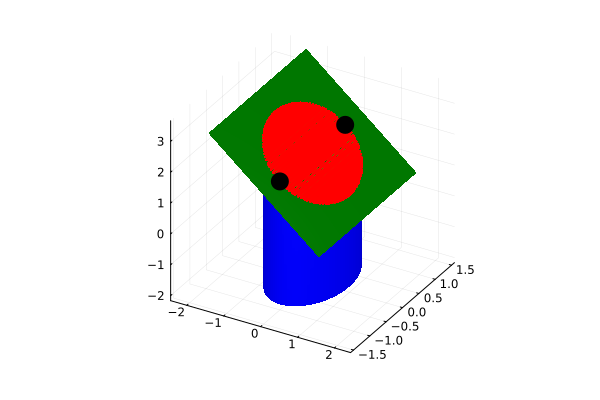
\includegraphics[width=0.7\columnwidth]{graphics/Chap06/CylinderPlaneTwoConstraints.png}
    \caption{The first constraint in Example~\ref{eq:LagrangeMultipliersTwoConstraints} gives a cylinder about the $z$-axis having radius one, while the second constraint defines a plane. The red elliptical/circular shape in the plane, excluding its interior, is the intersection of the two constraints, thereby defining the feasible set over which the cost is to be optimized. The two black points are the extrema, one corresponding to a maximum of $f(x, y, z) = x + y + z$ and the other to a minimum.}
    \label{fig:Constrained3LinkManipulator}
\end{figure}


\bigskip


\begin{example} 
\label{eq:LagrangeMultipliersTwoConstraints}
Maximize \( f(x, y, z) = (x + y + z) \) subject to the constraints \( x^2 + y^2 =1 \) and \( x + z = 2 \). The maximization is not a typo. We wish to illustrate our ``trick'' of minimizing the negative of the objective function.\\

The way we are approaching the problem, namely through Lagrange Multipliers, we can find all of the extreme points, whether we include the minus sign on the cost or not. With typical numerical solvers, this is not the case.
\end{example}

\textbf{Solution:} Though it is not required, we write down the constrained optimization problem,
\begin{align*}
\text{Minimize} \quad & f(x, y, z) = -(x + y + z)\\
\text{subject to} \quad & \begin{aligned}
\left[\begin{array}{c}
0 \\
0 
\end{array}\right] = \left[\begin{array}{c}
g_1(x, y, z) \\
g_2(x, y, z) 
\end{array}\right] 
= \left[\begin{array}{c}
x^2 + y^2 -1\\
x + z - 2
\end{array}\right] ,
\end{aligned}
\end{align*}
so as to make the identification of $f:\real^3 \to \real$ and $g:\real^3 \to \real^2$ crystal clear. Following the steps of Method~\ref{thm:MethodLagrangeMultipliersVectorized}, we define
$$L(x, y, z, \lambda_1, \lambda_2) = -(x + y + z) + \lambda_1(x^2 + y^2 -1) + \lambda_2(x + z - 2). $$

Taking the required partial derivatives, stacking them in a column, and setting them to zero, we obtain the stationary conditions,
\begin{equation}
\label{eq:gradientProblemTwoConstraints}
 \begin{aligned}
   0 &= \frac{ \partial L(x, y, z, \lambda_1, \lambda_2)}{\partial x} = -1 + 2 \lambda_1 \cdot x + \lambda_2 \\
   0 &= \frac{ \partial L(x, y, z, \lambda_1, \lambda_2)}{\partial y} = -1 + 2 \lambda_1 \cdot y \\
   0 &= \frac{ \partial L(x, y, z, \lambda_1, \lambda_2)}{\partial z} = -1 + \lambda_2 \\
    0 &= \frac{ \partial L(x, y, z, \lambda_1, \lambda_2)}{\partial \lambda_1} = x^2 + y^2 - 1 \\
    0 &= \frac{ \partial L(x, y, z, \lambda_1, \lambda_2)}{\partial \lambda_2} = x + z - 2.
\end{aligned}   
\end{equation}


Fortunately for us --\textbf{and it has to be like this for the problem to be doable by hand}-- we can solve for $x$, $y$, $z$, $\lambda_1$ and $\lambda_2$ using elementary algebraic manipulations. Indeed, 
\begin{align*}
\text{eqn \# 3:} ~~~&   0 = -1 +  \lambda_2  \implies \lambda_2 = 1\\
\text{eqn \# 1:} ~~~&      0 =2 \lambda_1 \cdot x  \implies x=0 ~~( \text{ because {eqn \# 2:} implies neither y nor}~\lambda_1 ~\text{ can equal zero})\\
 \text{eqn \# 5:} ~~~&     0 = x + z =- 2 \implies 0 = \frac{x}{y} \implies z = 2\\
 \text{eqn \# 4:} ~~~&      0 = x^2 + y^2 - 1  \implies y= \pm 1\\
 \text{eqn \# 2:} ~~~&      0 = -1 + 2 \lambda_1 \cdot y \implies \lambda_1= {\rm sign}(y) \cdot \frac{1}{2},\\
\end{align*}
where \text{eqn \# i:} corresponds to row i of \eqref{eq:gradientProblemTwoConstraints}. If there is a confusing point, it is the conclusion that \text{eqn \# 1:} implies $x=0$. This is true because if $\lambda_1 = 0$, then \text{eqn \# 2:} becomes $0 = -1$, which is impossible. Hence, $\lambda_1$
cannot be equal to zero, and hence, \text{eqn \# 1:} implies $x=0$. This is basic algebra. It's not fun math, perhaps, but still, just basic algebra. \textbf{Calculus gave us the equations; algebra is being used to solve them!}\\

Putting all of this together for the ``real'' cost function $f(x, y, z) = x + y + z$ we wanted to maximize, \textbf{the cost without the minus sign}, yields
$$\left[\begin{array}{c}
x^\ast\\
y ^\ast\\
z ^\ast\\
\lambda_1^\ast \\
\lambda_2^\ast \\
\end{array} \right] = \left[\begin{array}{c}
0 \\ 1 \\ 2 \\ \frac{1}{2} \\ 1
\end{array} \right] \text{giving a maximum of $f^\ast = 3$, and } \left[\begin{array}{c}
x^\ast\\
y ^\ast\\
z ^\ast\\
\lambda_1^\ast \\
\lambda_2^\ast \\
\end{array} \right] = \left[\begin{array}{r}
0 \\ -1 \\ 2 \\ -\frac{1}{2} \\ 1
\end{array} \right] \text{giving a minimum of $f^\ast = 1$}.$$

\Qed

\bigskip

\textbf{Let's now see how to do Lagrange Multipliers in code! The solution combines our ability to compute gradients symbolically, understand that stationary points correspond to roots of the gradient, and numerically solve root-finding problems. Not bad! This puts it all together. }

\bigskip

\begin{lstlisting}[language=Julia,style=mystyle]
using Symbolics, NLsolve, Random

# -------------------
# PROBLEM DEFINITION
# -------------------

# Define symbolic variables for the optimization
@variables var[1:3]  # Actual problem variables
@variables lam[1:2]  # Lagrange multipliers

# Objective function to be minimized
f = -(var[1] + var[2] + var[3])

# Constraint equations
g1 = var[1]^2 + var[2]^2 - 1
g2 = var[1] + var[3] - 2

# Formulate the Lagrangian: objective function + lagrange multipliers for constraints
L = f + lam[1]*g1 + lam[2]*g2

# Compute the gradient of the Lagrangian with respect to both variables and Lagrange multipliers
gradL = Symbolics.gradient(L, [var; lam])

# For debugging: display the gradient or convert it to LaTeX for better visualization
if false 
    display(gradL)
else
    latexify(gradL) |> println
end

# ---------------------------
# NUMERICAL SOLUTION APPROACH
# ---------------------------

# Convert the symbolic gradient expression to a numerical function for computational efficiency
gradL_num = build_function(gradL, [var; lam])
gradL_num = eval(gradL_num[1])

# Initialize an array to store solutions
f_solutions = Float64[]

# Solve the optimization problem for multiple initial guesses
# This is done to explore different solutions since NLsolve can get trapped in local minima
for k = 1:100
    # Generate a random initial guess for the optimization variables and Lagrange multipliers
    # randn is the normal or gaussian distribution, which includes positive and negative values
    initial_guess = randn(5)

    # Use nlsolve to find where the gradient is zero, which corresponds to an extremum
    result = nlsolve(gradL_num, initial_guess, xtol=1e-6, ftol=1e-7)


# Process the solution only if nlsolve successfully converged
if converged(result)
    # Extract the values of the problem variables from the solution
    var_val = result.zero[1:3]
    lam_val = result.zero[4:5]
    
    # Compute the value of the objective function at the found extremum
    f_extremePoint = -sum(var_val)
    
    # Add the found solution only if it is sufficiently different from the previously found solutions
    if all(abs(f_extremePoint - sol) > 1e-2 for sol in f_solutions)
        push!(f_solutions, f_extremePoint)
            @show [var_val; lam_val]
    end
end
end

# Sort solutions for easier analysis
sorted_solutions = sort(f_solutions)


\end{lstlisting}
\textbf{Output} 
\begin{equation}
\left[
\begin{array}{c}
-1.0000 + lam2 + 2.0000 lam1 var1 \\
-1.0000 + 2.0000 lam1 var2 \\
-1.0000 + lam2 \\
-1.0000 + var1^{2} + var2^{2} \\
-2.0000 + var1 + var3 \\
\end{array}
\right]
\end{equation}
\begin{verbatim}


[var_val; lam_val] = [2.5557001655682698e-9, -1.0000000021988782, 1.9999999974442995, 
    -0.4999999970071819, 1.0]
[var_val; lam_val] = [2.672589761676145e-12, 1.000000000001114, 1.9999999999973277, 
    0.49999999999892936, 1.0]
    
2-element Vector{Float64}:
 -3.000000000001114
 -0.9999999978011215
\end{verbatim}

\bigskip

\begin{rem} The above problem has two distinct roots. To which one will \texttt{NLsolve} converge? It depends on the initial condition. That is why the solver is run 100 times with random initial conditions, giving us a chance to find both of them.     
\end{rem}

\bigskip
Here is a solution using \texttt{Jump}. As a professional, this is preferred over the above solution using Lagrange Multipliers. Why? \textcolor{blue}{\bf Jump's code has been optimized for speed and tested by enough users that it is pretty bug-free}. For doing HW in Engineering courses, being able to run the symbolic version of Lagrange Multipliers will help you tremendously. Moreover, you now know several ways to check your HW and learn from your mistakes.\\

\begin{lstlisting}[language=Julia,style=mystyle]
using JuMP, Ipopt

# Create a new model with Ipopt as the solver
model = Model(Ipopt.Optimizer)

# Define the variables
@variable(model, var[1:3])

# Set the objective function
@NLobjective(model, Min, -(var[1] + var[2] + var[3]))

# Add the constraint equations
@NLconstraint(model, var[1]^2 + var[2]^2 == 1)
@NLconstraint(model, var[1] + var[3] == 2)

# Fine tune a few params
set_optimizer_attribute(model, "max_iter", 1000)  # Allow up to 1000 iterations
set_optimizer_attribute(model, "tol", 1e-9)      # Require a very accurate solution

# Suppress much of the output
set_optimizer_attribute(model, "print_level", 4)

# Solve the problem
optimize!(model)

# Display the results
println("Objective value: ", objective_value(model))
println("Solution: ")
println("var[1] = ", value(var[1]))
println("var[2] = ", value(var[2]))
println("var[3] = ", value(var[3]))

\end{lstlisting}
\textbf{Output} 
\begin{verbatim}
Total number of variables............................:        3
                     variables with only lower bounds:        0
                variables with lower and upper bounds:        0
                     variables with only upper bounds:        0
Total number of equality constraints.................:        2
Total number of inequality constraints...............:        0
        inequality constraints with only lower bounds:        0
   inequality constraints with lower and upper bounds:        0
        inequality constraints with only upper bounds:        0


Number of Iterations....: 15

                                   (scaled)                 (unscaled)
Objective...............:  -3.0000000000000000e+00   -3.0000000000000000e+00
Dual infeasibility......:   0.0000000000000000e+00    0.0000000000000000e+00
Constraint violation....:   0.0000000000000000e+00    0.0000000000000000e+00
Variable bound violation:   0.0000000000000000e+00    0.0000000000000000e+00
Complementarity.........:   0.0000000000000000e+00    0.0000000000000000e+00
Overall NLP error.......:   0.0000000000000000e+00    0.0000000000000000e+00


Number of objective function evaluations             = 16
Number of objective gradient evaluations             = 16
Number of equality constraint evaluations            = 16
Number of inequality constraint evaluations          = 0
Number of equality constraint Jacobian evaluations   = 16
Number of inequality constraint Jacobian evaluations = 0
Number of Lagrangian Hessian evaluations             = 15
Total seconds in IPOPT                               = 0.012

EXIT: Optimal Solution Found.
Objective value: -3.0
Solution: 
var[1] = 4.579141502905379e-17
var[2] = 1.0
var[3] = 2.0
\end{verbatim}


For our final example, we recover the solution to the underdetermined least squares problem treated in Chapter 9.9 of the ROB 101 \textit{Computational Linear Algebra} textbook.

\begin{example} Consider an underdetermined system of linear equations $Ax=b$, where $A$ is $m \times n$. When the rows of $A$ are linearly independent (equivalently, the columns of $A^\top$ are linearly independent), determine a minimum norm squared solution to $Ax = b$.    
\end{example}

\textbf{Solutions:} You know the routine: even though it is not required, we write down the constrained optimization problem 
\begin{align*}
\text{Minimize} \quad & f(x)=x \bullet x = x^\top \cdot x\\
\text{subject to} \quad & 0_{m \times 1} = g(x) = Ax -b,
\end{align*}
so as to make the identification of $f:\real^n \to \real$ and $g:\real^n \to \real^m$ crystal clear. Following the steps of Method~\ref{thm:MethodLagrangeMultipliers}, we define
$$L(x, \lambda):=x \bullet x + \lambda_1   (a_1 x - b_1) +  \lambda_2  (a_2 x - b_2) + \cdots + \lambda_m   (a_m x - b_m),$$
where $a_i$ are the rows of $A$ and $b_i$ are the entries of $b$. We then compute the required derivatives
\begin{align*}
     0_{n \times 1} & =\nabla (x \bullet  x) +  \lambda_1   \nabla (a_1 x - b_1) +  \lambda_2 \nabla  (a_2 x - b_2) + \cdots + \lambda_m   \nabla (a_m x - b_m) \\[1em]
     &= 2x +  \lambda_1 \cdot (a_1)^\top  +  \lambda_2 \cdot (a_2)^\top  + \cdots + \lambda_m   \cdot (a_m)^\top \\[1em]
     &= 2 x + A^\top  \cdot \lambda      \\[1em]
     0_{m\times 1} & = Ax - b.
\end{align*}
From the first $n$ equations, we obtain $x = -\frac{1}{2} A^\top \cdot \lambda$, and from the last $m$ equations we obtain the constraint, $Ax=b$. Substituting the first into the second and doing a bit of algebra yields
$$  \left(A \cdot A^\top \right) \cdot \lambda = -2 b.$$
Solving for $\lambda$ and substituting into $x = -\frac{1}{2} A^\top \cdot \lambda$ yields
$$ x = A^\top \cdot  \left(A \cdot A^\top \right)^{-1} \cdot b,$$
the same answer we had in ROB 101, namely,
\begin{equation}
\label{eq:MinNormUnderDetermined}
    x^\ast = \argmin_{Ax=b} ||x||^2 \iff x^\ast = A^\top\cdot (A \cdot A^\top)^{-1} b 
    \iff x^\ast = A^\top \alpha~~\text{and}~~A\cdot A^\top \alpha =b.
\end{equation}
Once we identify $\alpha = -\frac{1}{2} \lambda$, the correspondence is spot on. As in ROB 101, we recommend that the minimum norm squared solution be computed with the right-hand side of \eqref{eq:MinNormUnderDetermined} so that the matrix inverse is avoided, but for small problems, the middle answer is fine.
\Qed



\bigskip
\begin{figure}[ht]
    \centering
    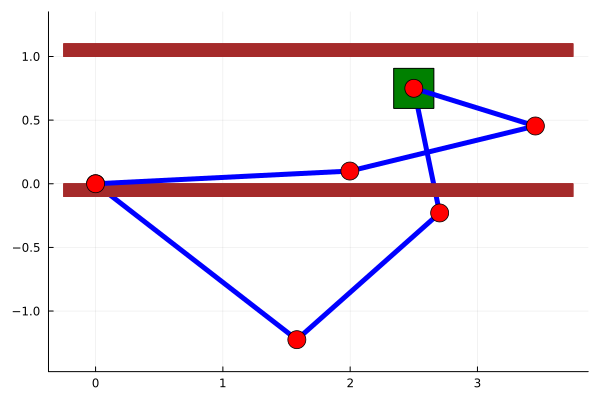
\includegraphics[width=0.7\columnwidth]{graphics/Chap06/constrainedInequalityOptimizationFor3LinkRobotKinematicChain.png}
    \caption{A pseudo-realistic manipulation task that requires inequality constraints in addition to equality constraints. The brown objects represent obstacles we must avoid while reaching into the green box with the robot's end effector. A solution with only equality constraints does reach into the green box, but ``pass through'' the obstacles. By adding inequality constraints, Jump finds the desired solution. The cost of the tightly constrained problem is approximately double of the other.}
    \label{fig:RealisticManipulationTasks}
\end{figure}


\bigskip

\subsection{3-Link Manipulator Meets Inequality Constraints}

We return to the three-link manipulator. Our goal is to place the end effector in a box, that will use \textbf{equality constraints}, and we want to avoid contacting an obstacle, which will use \textbf{inequality constraints}. We first set the problem up and then solve it using \texttt{Jump}.

A standard form for a constrained optimization problem includes both \textbf{equality and inequality constraints}. Many solvers require you to write the constraints in the form 
$$g^{\rm in}_j(x) \le 0, $$
as we show in \eqref{eq:GenericMultipleConstraintOptimizationProblemWithInequality}. Some solvers, such as \texttt{JuMP} do not make you jump through so many hoops (pun intended) and accept constraints in the form 
\begin{itemize}
    \item $g^{\rm in}_j(x) \le c_j$ \\
    \item $g^{\rm in}_j(x) < c_j$ \\
    \item $g^{\rm in}_j(x) > c_j$ \\
    \item $g^{\rm in}_j(x) \ge  c_j$. 
\end{itemize}

\textbf{Standard form for many Optimization Problems with inequality and equality constraints:}
\begin{equation}
\label{eq:GenericMultipleConstraintOptimizationProblemWithInequality}
\begin{aligned}
\text{Minimize} \quad & f(x)\\
\text{subject to} \quad & g^{\rm eq}_i(x) = 0, ~ 1\le i \le m,\\
        \quad & g^{\rm in}_j(x) \le 0, ~ 1\le j \le p,
\end{aligned}    
\end{equation}

For the 3-link manipulator, we'll take the cost function as 
$$f(\theta) = \left(\theta_1\right)^2 + \left(\theta_2\right)^2 + \left(\theta_3\right)^2.$$
We need two equality constraints to place the end effector in the box located at $(3.5, 0)$, namely
\begin{align*}
    g^{\rm eq}(\theta) = \left[ \begin{array}{c} 
   g^{\rm eq}_1(\theta)\\  
    g^{\rm eq}_2(\theta)
    \end{array} \right] =  \left[ \begin{array}{c} 
    L1 \cdot \cos(\theta_1) + L2 \cdot \cos(\theta_1 + \theta_2) + L3 \cdot \cos(\theta_1 + \theta_2 + \theta_3) - 3.5 \\  
    L1 \cdot \sin(\theta_1) + L2 \cdot \sin(\theta_1 + \theta_2) + L3 \cdot \sin(\theta_1 + \theta_2 + \theta_3) -0.0  \end{array} \right], 
\end{align*}
and we'll impose four inequality constraints on the vertical components of $p_1$ and $p_2$ of the robot, namely,
\begin{align*}
    g^{\rm in}(\theta) = \left[ \begin{array}{l} 
   g^{\rm in}_1(\theta)\\  
    g^{\rm in}_2(\theta) \\
       g^{\rm in}_3(\theta)\\  
    g^{\rm in}_2(\theta) \\
    \end{array} \right] =  \left[ \begin{array}{c} 
    L1 \cdot \sin(\theta_1) \ge 0.1\\  
    L1 \cdot \sin(\theta_1) + L2 \cdot \sin(\theta_1 + \theta_2) \ge 0.1  \\
     L1 \cdot \sin(\theta_1) \le 0.95\\  
    L1 \cdot \sin(\theta_1) + L2 \cdot \sin(\theta_1 + \theta_2) \le 0.95  \end{array} \right]. 
\end{align*}
We do not impose constraints on their horizontal positions because we don't care where the joints end up. We simply want the links to be above the obstacle.

\bigskip
Here is what it looks like in \texttt{JuMP}
\bigskip

\begin{lstlisting}[language=Julia,style=mystyle]
# JuMP solves the problem 
using Plots, JuMP, Ipopt

# Define the model parameters for the robot manipulator
function modelParameters()
    # Lengths of the three links
    L1, L2, L3 = [2, 1.5, 1]
    return (L1=L1, L2=L2, L3=L3)
end

# Calculate the positions of the robot's links based on the joint angles
function linkPostions(th1,th2,th3)
    params = modelParameters()
    # Base position
    p0 = [0.0; 0.0]
    # Calculate positions of the other joints
    p1 = p0 + [params.L1 * cos(th1); params.L1 * sin(th1)]
    p2 = p1 + [params.L2 * cos(th1+th2); params.L2 * sin(th1+th2)]
    p3 = p2 + [params.L3 * cos(th1+th2+th3); params.L3 * sin(th1+th2+th3)]
    return (p0=p0, p1=p1, p2=p2, p3=p3)
end

# Plot a rectangle on the current plot
function plot_rectangle(xc, yc, w, h; color="brown")
    # Calculate the corners of the rectangle
    x1 = xc - w/2
    x2 = xc + w/2
    y1 = yc
    y2 = yc + h
    # Plot the rectangle
    plot!([x1, x2, x2, x1, x1], [y1, y1, y2, y2, y1], fill=true, fillalpha=1.0, 
    fillcolor=color, linecolor=color, legend=false)
end

# Plot the robot's configuration
function plot_points(positions, label; line_thickness=5, ball_size=10)
    # Extract joint positions
    p0 = positions.p0
    p1 = positions.p1
    p2 = positions.p2
    p3 = positions.p3   
    # Plot obstacles
    plot_rectangle(1.75, 1, 4, .1)
    plot_rectangle(1.75, -.1, 4, .1)
    # Plot the robot's configuration
    scatter!([p3[1]], [p3[2]], color=:green, markersize=2*ball_size, marker=:square, label=nothing)  
    plot!([p0[1], p1[1], p2[1], p3[1]], [p0[2], p1[2], p2[2], p3[2]], 
        linewidth=line_thickness, color=:blue, label=label)        
    scatter!([p0[1], p1[1], p2[1], p3[1]], [p0[2], p1[2], p2[2], p3[2]], color=:red, markersize=ball_size, label=nothing)
end

# Solve the optimization problem and plot the solution
function solve_and_plot(use_inequality_constraints)
    params = modelParameters()
    model = Model(Ipopt.Optimizer)
    # Solver settings
    set_optimizer_attribute(model, "max_iter", 1000)
    set_optimizer_attribute(model, "tol", 1e-9)
    set_optimizer_attribute(model, "print_level", 1)
    # Define optimization variables and constraints
    @variable(model, -π<= th1 <= π)
    @variable(model, -π <= th2 <= π)
    @variable(model, -π <= th3 <= π)
    @constraint(model, g1, params.L1*cos(th1) + params.L2*cos(th1 + th2) + params.L3*cos(th1 + th2 + th3) - 2.5 == 0)
    @constraint(model, g2, params.L1*sin(th1) + params.L2*sin(th1 + th2) + params.L3*sin(th1 + th2 + th3) - 0.75 == 0)
    if use_inequality_constraints
        @constraint(model, g3, params.L1*sin(th1) <= 0.95)
        @constraint(model, g4, params.L1*sin(th1) + params.L2*sin(th1 + th2) <= 0.95)
        @constraint(model, g5, params.L1*sin(th1) >=0.1)
        @constraint(model, g6, params.L1*sin(th1) + params.L2*sin(th1 + th2) >=0.1)
    end
    # Define the objective function
    @objective(model, Min, th1^2 + th2^2 +  th3^2)
    # Solve the optimization problem
    optimize!(model)
    # Display the results
    label = use_inequality_constraints ? "With Inequality Constraints" : "No Inequality Constraints"
    println(label) 
    println("Objective value: ", objective_value(model))
    println("Solution: ")
    println("th1Star = ", value(th1))
    println("th2Star = ", value(th2))
    println("th3Star = ", value(th3))
    println(" ")            
    positions = linkPostions(value(th1), value(th2), value(th3))
    plot_points(positions, label)
end

# Initialize the plot
fig = plot(; aspect_ratio=:equal, legend=false)
# Solve and plot without and with inequality constraints
solve_and_plot(false)
solve_and_plot(true)
# Display and save the plot
display(fig)
png(fig, "constrainedInequalityOptimizationFor3LinkRobotKinematicChain")

\end{lstlisting}
\textbf{Output} (Angles in radians)
\begin{verbatim}
No Inequality Constraints
Objective value: 3.4536798144131877
Solution: 
th1Star = -0.6590530918483652
th2Star = 1.3848362097307525
th3Star = 1.0495510986878442
 
With Inequality Constraints
Objective value: 6.812490744951165
Solution: 
th1Star = 0.05002085181111906
th2Star = 0.18815229215108328
th3Star = 2.6028037525509964
\end{verbatim}
The configuration of the robot is shown Fig.~\ref{fig:RealisticManipulationTasks}.

% \begin{lstlisting}[language=Julia,style=mystyle]

% \end{lstlisting}
% \textbf{Output} 
% \begin{verbatim}

% \end{verbatim}

\bigskip

\begin{figure}[htb]%
\centering
\subfloat[]{%
%\includegraphics[trim=7cm 1cm 7cm 1cm, clip, width=0.45\columnwidth]
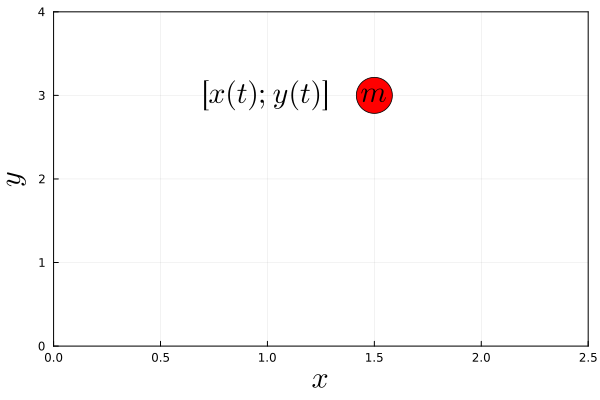
\includegraphics[width=0.45\columnwidth]{graphics/Chap06/Point_Mass.png}}%
%\hfill%
\hspace{.3cm}
\subfloat[]{%
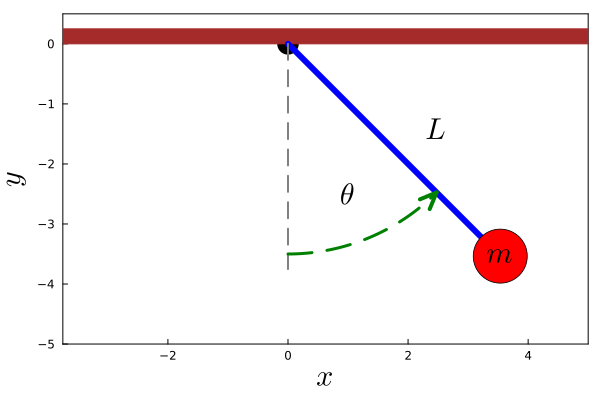
\includegraphics[ width=0.45\columnwidth]{graphics/Chap06/Pendulum.png}}%
\hfill
\caption[]{(a) A point mass in the plane with its Cartesian coordinates. The origin is in the bottom left corner.(b) The classic pendulum formed by a massless rod with a point mass attached at its end. The angle $\theta$ is measured CCW from the vertical. The origin is placed at the pivot point attached to the ``ceiling''.}
    \label{fig:SimplestDynamics}
\end{figure}

% \begin{figure}[ht]
%     \centering
%     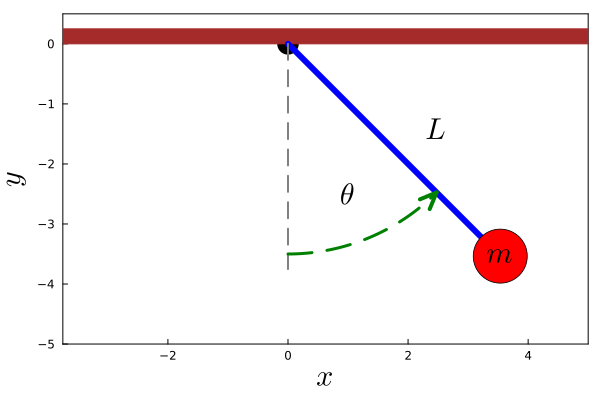
\includegraphics[width=0.45\columnwidth]{graphics/Chap06/Pendulum.png}
%     \caption{The classic pendulum formed by a massless rod with a point mass attached at its end. The angle $\theta$ is measured CCW from the vertical. The origin is placed at the pivot point attached to the ``ceiling''.}
%     \label{fig:PedulumBob}
% \end{figure}


\section{Dynamics \`a la Lagrange}
\label{sec:LagrangianDynamics}

You know for sure that $F = m \cdot a$ for a point mass, as shown in Fig.~\ref{fig:SimplestDynamics}-(a), and you've likely seen the equation for the pendulum of Fig.~\ref{fig:SimplestDynamics}-(b),
\begin{equation}
\label{eq:IdealPendulum}
  \ddot{\theta}(t) = - \frac{g}{L} \cdot \sin(\theta).  
\end{equation}
But could you derive the equations for a person riding a \href{https://youtu.be/nA6vofrLypg}{Hoverboard}? Or the 3-link manipulator in Fig.~\ref{fig:RobotAbsoluteAngle}-(b)? At the end of this section, you will be able to do all of this and more. You'll be able to derive by hand the equations for simple models such as the pendulum, and, via the \texttt{Symbolics} package, handle more complicated models. 

\bigskip

\begin{funColor}{Fun Facts about Lagrange}{LagrangeFun}
 \href{https://en.wikipedia.org/wiki/Joseph-Louis_Lagrange}{Joseph-Louis Lagrange} (1736–1813) did not have the advantage of computers or modern software to assist with computations, as we do today. In his time, mathematics was done by hand using pen and paper. Though some mathematicians had colleagues or students with whom they might discuss ideas or collaborate on problems, they didn't have ``assistants'' in the sense of someone performing computational tasks for them.\\
 
 \textbf{Oh yeah, the Fun Facts:} Lagrange was largely self-taught and did not obtain a university degree. Fascinated by maxima and minima of functions, he was the principal founder of the calculus of variations. In a far-reaching reformulation of Isaac Newton's laws, Lagrange created a brilliant new vision of mechanics. We are working toward that now in this Section! \\

 \textbf{ChatGPT's Remarks on the Fun Facts: } The statement is mostly accurate, and here's a deeper analysis of its points:

\begin{enumerate}
    \item \textbf{Self-taught}: Lagrange was largely self-taught in his early mathematical education. He exhibited an innate interest in mathematics from a tender age and initiated his study autonomously. 
    
    \item \textbf{University Degree}: While it's true that the nature of formal education in the 18th century was distinct from today, Lagrange did not follow the prototypical academic trajectory that we associate with eminent mathematicians today. Nevertheless, by the age of 19, he was already delivering significant papers to the mathematical domain. His pioneering contributions were acknowledged early, leading him to assume several esteemed academic roles throughout his life.
    
    \item \textbf{Calculus of Variations}: Indeed, Lagrange made seminal contributions to the calculus of variations. He held a specific intrigue for the problem of the brachistochrone, which pertains to the quickest descent path under the influence of gravity. This inquiry propelled him to devise what is contemporarily referred to as the Euler-Lagrange equation, pivotal in the calculus of variations.
    
    \item \textbf{Reformulation of Newton's Laws}: In his magnum opus ``Mécanique Analytique'', Lagrange made profound contributions to mechanics. Within, he presented a novel interpretation of classical mechanics rooted entirely in energy principles, laying the groundwork for the Lagrangian mechanics we recognize today. This methodology deploys a singular scalar entity, termed the Lagrangian, to elucidate system dynamics, as opposed to the vectorial forces characteristic of Newtonian mechanics. Lagrange's conceptualization offers a more holistic and adaptable perspective, especially pertinent for intricate systems and scenarios.
\end{enumerate}

In summation, while the provided statement offers a concise encapsulation of Lagrange's achievements and background, the life and contributions of such a distinguished individual warrant a more detailed exploration. Thank you, ChatGPT!
10 Oct. 2023.
\end{funColor}

% \jwg{Note to self and IA team: now that I have center of mass carefully covered, we can add distributed mass in a Julia HW problem. Adding the moment of inertia will be informative. Talk to me for ideas.}

\subsection{The Dot Notation for Derivatives}

In \eqref{eq:IdealPendulum}, $\ddot{\theta}(t)$ denotes the \textbf{angular acceleration} of the pendulum. The dot notation for derivatives is a very popular quasi-standard notation for denoting derivatives with respect to time. For example, if the vector
\begin{equation}
\label{eq:CartesianPosition}
  p(t):=\left[
\begin{array}{c}
x(t)\\
y(t)\\
\end{array}
\right]  
\end{equation}
is the Cartesian position of the particle in the plane, then its 
Cartesian \textbf{velocity} is the first derivative with respect to time of the position vector, namely,
\begin{equation}
\label{eq:CartesianVelocity}
v(t):=\left[
\begin{array}{c}
\dot x(t)\\
\dot y(t)\\
\end{array}
\right]:= \frac{d}{dt}  \left[
\begin{array}{c}
x(t)\\
y(t)\\
\end{array}
\right] = \left[ \begin{array}{c}
\frac{ dx(t)}{dt}\\
\frac{d y(t)}{dt}\\
\end{array}
\right], 
\end{equation}
read as $x$ and $y$ dot. In a similar manner, the derivative of the velocity vector with respect to time is the Cartesian \textbf{acceleration vector}, 
\begin{equation}
\label{eq:CartesianAcceleration}
a(t):=\left[
\begin{array}{c}
\ddot x(t)\\
\ddot y(t)\\
\end{array}
\right]:= \frac{d}{dt} \left[
\begin{array}{c}
\dot x(t)\\
\dot y(t)\\
\end{array}
\right] =  \left[ \begin{array}{c}
\frac{ d^2x(t)}{dt^2}\\
\frac{d^2 y(t)}{dt^2}\\
\end{array}
\right] 
\end{equation}
read as $x$ and $y$ double dot.

For a point mass in the plane, as in Fig.~\ref{fig:SimplestDynamics}-(a), with its Cartesian position, velocity, and acceleration given in \eqref{eq:CartesianPosition} to \eqref{eq:CartesianAcceleration}, you may recall from a Physics course (and if not, please accept this for a fact), that when the only force acting on the mass is gravity, $g= 9.81 \frac{\rm m}{\rm s^2}$, Newton's laws give
\begin{equation}
 \left[   
 \begin{array}{c}
m \cdot \ddot{x}(t) \\
m \cdot \ddot{y}(t) \\
\end{array}
\right] = \left[
\begin{array}{c}
0.0 \\
- m \cdot g \\
\end{array}
\right].
\end{equation}
Equations like this are also called the \textbf{equations of motion} or EoM for short. The equations of motion for the \href{https://www.youtube.com/playlist?list=PLFe0SMV3hBCBPg0dDG9FbqOy_x7H9kEDJ}{Cassie bipedal robot} are ``somewhat'' similar to the above, except they would fill 100 pages!

We will not need the third derivative with respect to time in this Section, but you might note that it is called the \href{https://en.wikipedia.org/wiki/Jerk_(physics)}{jerk}. Car and elevator manufacturers are very careful about the ``smoothness of acceleration'' (keeping its rate of change continuous and not too large), so they use bounds on  \textbf{jerk}, the third derivative of position, in the design of their products. When you see clothing\footnote{Easily available on the web. Here, three dots would be too subtle.} with \begin{center}
    \textbf{\large ``Don't be a $\bm{\frac{d^3 x(t)}{dt^3}}$''},
\end{center} 
you are now in the know. 

\subsection{Kinetic and Potential Energy of a Point Mass in the Plane}
\label{sec:KineticPotentialEnergyPointMass}


We define:
\begin{itemize}
    \item \textbf{Potential Energy of a Point Mass} is equal to ``mass times gravity times height'', or in symbols
    $$V:= m \cdot g \cdot y,$$
    where we have deliberately dropped the explicit dependence on time; keep in mind, however, that the particle's height does vary with time.

    \item \textbf{Kinetic Energy of a Point Mass} by ``one half mass times the magnitude (or norm) of the velocity squared'', or in symbols,
    \begin{equation}
    \label{eq:KEpointMassNoConstraints}
        K:= \frac{1}{2} m \cdot\left( \dot{x}^2  +  \dot{y}^2 \right),
    \end{equation}
     where, again, we have deliberately dropped the explicit dependence on time; keep in mind, however, that the particle's velocity does vary with time.
\end{itemize}
For later use, we note that both the potential and kinetic energies are scalar quantities. Their units are \href{https://en.wikipedia.org/wiki/Joule}{Joules}. We will not make a big deal about units, though they are very important. \textbf{We do want to observe that the kinetic energy is quadratic in the velocity components of the particle.} In fact, the Cartesian velocity, $v(t)$, is a 2-vector (because we are working in the plane) and its kinetic energy is $$K:=\frac{1}{2} m \cdot ||v(t)||^2.$$ 
We note this, so that in 3-space, you know how to compute the kinetic energy of a point mass! It is always the same formula: one-half the mass times the norm of the velocity squared.

This all looks very innocent and perhaps a touch boring. For an unconstrained particle in the plane, computing potential and kinetic energy is absolutely cake! Let's consider, instead, the pendulum, which has a mass attached to a massless rod. We emphasize that the rod is massless because it then has no potential or kinetic energy. The potential and kinetic energies of the pendulum reside solely in the bob of mass $m>0$.

Just as we did with the 3-link robot in Chapter\ref{sec:ThreeLinkRobot}, we use basic trigonometry to write down the Cartesian position of the bob, namely,
\begin{equation}
\label{eq:PendulumPosition}
    p = \left[\begin{array}{r} x \\ y \end{array}\right] = \left[\begin{array}{c} L \cdot \sin(\theta) \\ - L \cdot \cos(\theta)\end{array}\right].
\end{equation}
The sines and cosines show up in different places because the angle $\theta$ for the pendulum is now referenced with respect to the vertical, with $\theta = 0$ corresponding to straight down, i.e., the pendulum at rest. We can now compute the potential energy for the pendulum,
\begin{equation}
    V_{\rm pend} = m \cdot g \cdot y =  - m \cdot g \cdot L \cdot \cos(\theta).
\end{equation}
The potential energy is at its lowest when the pendulum is hanging downwards and at its peak when the pendulum has rotated to $\theta = \pi$, straight up. Moreover, the potential energy is a nonlinear function of $\theta$

To determine the kinetic energy of the pendulum's bob, we must differentiate the position, namely,
\begin{equation}
\label{eq:PendulumVelocity}
    v = \left[\begin{array}{r} \dot{x} \\ \dot{y} \end{array}\right] = 
    \left[\begin{array}{c} \frac{d}{dt}  \left( L \cdot \sin(\theta) \right)\\ \frac{d}{dt} \left(- L  \cdot  \cos(\theta)  \right)\end{array}\right] = 
    \left[\begin{array}{c} L \cdot \cos(\theta) \cdot \dot{\theta}\\ 
    L \cdot \sin(\theta) \cdot \dot{\theta}\end{array}\right],
\end{equation}
where we used the chain rule. For the moment, let's accept the velocity calculation as being correct, and compute the kinetic energy,
\begin{equation}
\label{eq:KEpendulum}
\begin{aligned}
    K_{\rm pend} &= \frac{1}{2} m \cdot \left( (\dot{x})^2 + (\dot{y})^2) \right) \\
    & =  \frac{1}{2} m \cdot \left( (L \cdot \cos(\theta) \cdot \dot{\theta})^2 + (L \cdot \sin(\theta) \cdot \dot{\theta})^2) \right) ~~(\text{substituting in})\\
     &= \frac{1}{2} m \cdot L^2 \cdot \left( \cos^2(\theta) + \sin^2(\theta) \right) \cdot \dot{\theta}^2 ~~(\text{algebra})\\
     &= \frac{1}{2} m \cdot L^2 \cdot \dot{\theta}^2 ~~(\text{using the one trig identity everyone knows}).
\end{aligned}
\end{equation}
The kinetic energy is now quadratic function of the \textbf{angular velocity}, $\dot{\theta}$. The kinematics of the pendulum are specified by a single quantity, its angle $\theta$, and the time rate of change of that quantity shows up in the kinetic energy. 

\textbf{The Chain Rule:} We come back to computing $\dot{x}$ and $\dot{y}$ in \eqref{eq:PendulumVelocity}. 
\begin{itemize}
    \item We need to differentiate $x(t)= L \cdot \sin(t)$ with respect to time, $t$. \\
    
    Define $f:\real \to \real$, by $f(z) = \sin(z)$ and $g:\real \to \real$ by $g(t) = \theta(t)$. Then $x(t) = f(g(t))$; yes, $z$ in $f(z)$ is substituted in by $g(t) = \theta(t)$. By the Chain Rule, using the prime notation for differentiation,
    $$ \dot{x}(t) = x'(t) = L \cdot \left( f(g(t)) \right)' = L \cdot f'(g(t)) \cdot g'(t).$$
    We compute the various terms,
    \begin{align*}
        f'(z) & = (\sin(z))' = \cos(z) \\
        g'(t)& = (\theta(t))' = \frac{d}{dt} \theta(t) = \dot{\theta}(t).
    \end{align*}
    Putting the pieces together yields,
       \begin{align*}
        \dot{x}(t) & = L \cdot f'(g(t)) \cdot g'(t) \\
        &= L \cdot \sin(g(t)) \cdot g'(t)\\
        & L \cdot \sin(\theta(t)) \cdot \dot{\theta}(t) \\
        & = L \cdot \sin(\theta) \cdot \dot{\theta} ~~\text{after dropping the t's}.
    \end{align*}
    Professionals drop the t's because they know they are there and carrying them along for the ride in the derivations is ``heavy''.

    You may not need the next one, but a minus sign does disappear, and it's good to see how that happens.

    \item We need to differentiate $y(t)= -L \cdot \cos(t)$ with respect to time, $t$. \\ 
    
    Define $f:\real \to \real$, by $f(z) = \cos(z)$ and $g:\real \to \real$ by $g(t) = \theta(t)$. Then $y(t) = f(g(t))$; again, $z$ in $f(z)$ is substituted in by $g(t) = \theta(t)$. By the Chain Rule, using the prime notation for differentiation,
    $$ \dot{y}(t) = y'(t) = -L \cdot \left( f(g(t)) \right)' =- L \cdot f'(g(t)) \cdot g'(t).$$
    We compute the various terms,
    \begin{align*}
        f'(z) & = (\cos(z))' = - \sin(z) \\
        g'(t)& = (\theta(t))' = \frac{d}{dt} \theta(t) = \dot{\theta}(t).
    \end{align*}
    Putting the pieces together yields,
       \begin{align*}
        \dot{y}(t) & = - L \cdot f'(g(t)) \cdot g'(t) \\
        &= -L \cdot (- \sin(g(t)) ) \cdot g'(t)\\
        &= L \cdot \sin(\theta(t)) \cdot \dot{\theta}(t)  ~~(\text{double minus sign cancelled)})\\
        & = L \cdot \sin(\theta) \cdot \dot{\theta} ~~\text{after dropping the t's}.
    \end{align*}

    In the next part, we'll compute the potential and kinetic energies of the 3-link robot. While it can be done by hand, it's so painful that we will approach it symbolically. This will put you one step closer to how real dynamical models of engineering systems are determined.
    
\end{itemize}

\subsection{Kinetic and Potential Energy of the 3-Link Manipulator}

Just as with the pendulum, we assume the links of the robot are massless\footnote{A bad assumption in practice, but a good one for learning.} except for point masses $m_i>0$ at the ends of each link; the red balls in Fig.~\ref{fig:RobotAbsoluteAngle}-(b) and Fig.~\ref{fig:robotKinematicsConstrainedOptimization}. 

The kinetic energy functions become quite complex quite quickly! Hence, as a warm-up exercise, we leave off the third link in the manipulator, giving us a 2-link robot. To set us up for \textbf{Lagrange's Method} in the next section (yes, him again! what an amazing mathematician.), we're going to use what are called \textbf{generalized coordinates}, where we replace
\begin{align*}
    \theta_1 &\to q_1 \\
    \theta_2 &\to q_2\\
    \theta_3 &\to q_3.
\end{align*}
Even for the 2-link version of the robot, the kinetic energy will not fit on one line! Fortunately for us Engineers, kinetic energy has some beautiful structure, which we highlight in the following result.

\begin{propColor}{Kinetic Energy is a Quadratic Form}{KineticEnergyQuadraticForm}

The kinetic energy of any robot comprised of rigid links (e.g., our 3-link manipulator) can be expressed in the following quadratic form 
\begin{equation}
    \label{eq:KEwithMassInertiaMatrix}
    K(q, \dot{q}) = \frac{1}{2} \dot{q}_1^\top D(q) \dot{q},
\end{equation}
where $$ \left[ \begin{array}{c} q_1 \\  q_2 \\ \vdots \\ q_n \end{array} \right] \text{ and } \left[ \begin{array}{c} \dot{q}_1 \\  \dot{q}_2 \\ \vdots \\ \dot{q}_n \end{array} \right]$$
are the generalized position and velocity coordinates, respectively, and 
\begin{equation}
    \label{eq:MassInertiaMatrix}
    D(q) = \left[ \begin{array}{cccc} 
    d_{11}(q) &  d_{12}(q) & \cdots &  d_{1n}(q) \\  
    d_{21}(q) &  d_{22}(q) & \cdots &  d_{2n}(q) \\ 
    \vdots & \vdots & \ddots & \vdots \\
    d_{n1}(q) &  d_{n2}(q) & \cdots &  d_{nn}(q)     
    \end{array} \right] 
\end{equation}
is a \textbf{positive-definite\footnote{All eigenvalues are positive real numbers is the characterization we used in ROB 101 \textit{Computational Linear Algebra}. The Appendix of the ROB 101 textbook has a deeper treatment of positive definite matrices, in case you are curious.} symmetric matrix}. \\

$D(q)$ is called the \textbf{mass-inertia matrix}. \textbf{Its determinant is always positive (meaning greater than zero), and hence $D(q)$ is always invertible.}   
\end{propColor}

\subsubsection{Warm-up Problems}

\begin{example} Determine the mass-inertia matrices for the systems in Fig.~\ref{fig:SimplestDynamics}, that is, a point mass in the plane moving under the influence of gravity and a pendulum consisting of a point mass at the end of a massless bar.
\end{example}
\textbf{Solutions:}

For Fig.~\ref{fig:SimplestDynamics}-(a), we defined the kinetic energy in \eqref{eq:KEpointMassNoConstraints}. All we have to do is write it in the form \eqref{eq:KEwithMassInertiaMatrix}. Doing so yields
\begin{align*}
    K & = \frac{1}{2} m \cdot\left( \dot{x}^2  +  \dot{y}^2 \right) \\
    & = \frac{1}{2} \left[ \begin{array}{c} \dot{x} \\  \dot{y}\end{array} \right]^\top \cdot  
    \left[ \begin{array}{cc} 
    m &  0 \\  
    0 & m    
    \end{array} \right]
    \cdot \left[ \begin{array}{c} \dot{x} \\  \dot{y}\end{array} \right].
\end{align*} 
Hence, 
$$ D(x, y) = 
    \left[ \begin{array}{cc} 
    m &  0 \\  
    0 & m    
    \end{array} \right],$$
a diagonal matrix with the mass on the diagonal. Not so interesting, except it is clearly symmetric and positive definite as long as $m>0$!\\

For Fig.~\ref{fig:SimplestDynamics}-(b), we computed in \eqref{eq:KEpendulum} that 
$$ {KE}_{\rm pend} = \frac{1}{2} m \cdot L^2 \cdot \dot{\theta}^2.$$
Hence, 
$$D(\theta) = m \cdot L^2, $$
a $1 \times 1$ matrix depending on mass and length. Not so interesting, except it is clearly symmetric and positive definite as long as $m>0$ and $L >0$.\\

Will the multi-link robots be more interesting? In fact, they will be so interesting that writing $KE$ by hand in the form of \eqref{eq:KEwithMassInertiaMatrix} will be highly error-prone. 

\vspace{.2cm}

\begin{methodColor}{Recovering the Mass-Inertia Matrix from the Kinetic Energy}{RecoveringMassInertiaMatrix}
    Given an arbitrarily complicated (correct) expression $KE(q, \dot{q})$ for the Kinetic Energy of a rigid $n$-link mechanism, the mass-intertia matrix can be extracted via a double Jacobian, that is, 
    $$D(q) = \frac{\partial}{\partial \dot{q}} \left[ \left( \frac{\partial}{\partial \dot{q}} KE(q, \dot{q}) \right)^\top \right]. $$

\textbf{Note:}  This follows from part (f) of Prop.~\ref{thm:MatrixVectorCalculusFormulas}  in Chapter~\ref{sec:MoreMatrixVectorCalculus}, which is optional reading. Hence, \textbf{you are not expected to go check it out, unless you are really into the math}. We'll give you the required symbolic code to compute $D(q)$. When you see the double Jacobian, we wanted you to know what's up. Enough said. 
\end{methodColor}

\Qed

\subsubsection{Final Warm-Up Problem, a 2-Link Manipulator}

Here is the Symbolic code for computing the energies of a two-link robot.

\vspace{.2cm}

\begin{lstlisting}[language=Julia,style=mystyle]
using Symbolics, SymPy, Latexify
set_default(fmt = "%.1f", convert_unicode = false)
#latexify(b) |> println

# This is for a two-link manipulator

# For the angles, see the schematic of the 3-link manipulator
# and remove the last link

@Symbolics.variables q1 q2 dq1 dq2 g m1 m2 L1 L2

# We have substituted theta1 and theta2 by q1 and q2
# Not only is this more compact, but it's also
# standard notation for Lagrange's Method for computing
# dynamical equations of motion

# Form vectors for use in Jacobians
q = [q1, q2]
dq = [dq1, dq2]

# Kinematics
p1 = L1*[cos(q1), sin(q1)]
p2 = p1 + L2*[cos(q1+q2), sin(q1+q2)]

# Potential Energy
PE = g*m1*p1[2] + g*m2*p2[2]
PE = simple(PE)
println("PE = ", PE)

# Velocity vectors via the Jacobian!
v1 = Symbolics.jacobian(p1, q) * dq
v2 = Symbolics.jacobian(p2, q) * dq

# Kinetic Energy of each mass on the Robot
KE1 = 0.5 * m1 * sum(v1.*v1) 
KE2 = 0.5 * m2 * sum(v2.*v2)

# Sum the individual KEs to get the total Kinetic Energy
KE = KE1 + KE2

# Extract the mass-inertia matrix from KE
if false
    D = Symbolics.jacobian(Symbolics.jacobian([KE], dq), dq)
else
    D = Symbolics.hessian(KE, dq)
end

D = simple(D)
# Choose display method for the mass-inertia matrix
if false
    print("D = ")
    display(D)
else
    n= size(D,1)
    for i = 1:n
        for j = i:n
            print("\n \n D[$i,$j] = ", D[i,j])
        end
    end
end
\end{lstlisting}
\textbf{Output After Simplication Using a Custom Function Developed in Collaboration with ChatGPT4, 09 to 14 Oct 2023. More on this later.} 
\begin{verbatim}
PE = g*(L1*m1*sin(q1) + m2*(L1*sin(q1) + L2*sin(q1 + q2)))

 
 D[1,1] = L1^2*m1 + m2*(L1^2 + 2*L1*L2*cos(q2) + L2^2)
 
 D[1,2] = L2*m2*(L1*cos(q2) + L2)
 
 D[2,2] = L2^2*m2
 D[2,2] = L2^2*m2
\end{verbatim}

\textbf{Typeset Mass-intertia Matrix}
\begin{equation} D(q) =\left[\begin{array}{cc}L_{1}^{2} \cdot m_{1} + m_{2} \cdot \left( L_{1}^{2} + 2 \cdot L_{1} \cdot L_{2} \cdot \cos\left( q_{2} \right) + L_{2}^{2} \right) & L_{2} \cdot m_{2} \cdot \left( L_{1} \cdot \cos\left( q_{2} \right) + L_{2} \right) \\L_{2} \cdot m_{2} \cdot \left( L_{1} \cdot \cos\left( q_{2} \right) + L_{2} \right) & L_{2}^{2} \cdot m_{2} \\\end{array}\right];\end{equation}
this is a more interesting mass-inertia matrix! We are done with the warmup.

\subsubsection{3-Link Manipulator: The Real Deal}
\begin{lstlisting}[language=Julia,style=mystyle]
using Symbolics, SymPy, Latexify
set_default(fmt = "%.1f", convert_unicode = false)
#latexify(b) |> println

# This is for a three-link manipulator

# For the angles, see the schematic of the 3-link manipulator
# and remove the last link

@Symbolics.variables q1 q2 q3 dq1 dq2 dq2 dq3 g m1 m2 m3 L1 L2 L3

# We have substituted theta_i by q_i
# Not only is this more compact, but it's also
# standard notation for Lagrange's Method for computing
# dynamical equations of motion

# Form vectors for use in Jacobians
q = [q1, q2, q3]
dq = [dq1, dq2, dq3]

# Kinematics
p1 = L1*[cos(q1), sin(q1)]
p2 = p1 + L2*[cos(q1+q2), sin(q1+q2)]
p3 = p2 + L3*[cos(q1+q2+q3), sin(q1+q2+q3)]

# Potential Energy
PE = g*m1*p1[2] + g*m2*p2[2] + g*m3*p3[2]
PE = simple(PE)
println("PE = ", PE)

# Velocity vectors via the Jacobian!
v1 = Symbolics.jacobian(p1, q) * dq
v2 = Symbolics.jacobian(p2, q) * dq
v3 = Symbolics.jacobian(p3, q) * dq

# Kinetic Energy of each mass on the Robot
KE1 = 0.5 * m1 * sum(v1.*v1) 
KE2 = 0.5 * m2 * sum(v2.*v2)
KE3 = 0.5 * m3 * sum(v3.*v3)

# Sum the individual KEs to get the total Kinetic Energy
KE = KE1 + KE2 + KE3
KE = Symbolics.simplify(KE)

# Extract the mass-inertia matrix from KE
if false
    D = Symbolics.jacobian(Symbolics.jacobian([KE], dq), dq)
else
    D = Symbolics.hessian(KE, dq)
end

# Do simplification on D with a custom function 
D = simple(D)

# Choose display method for the mass-inertia matrix
if false
    print("D = ")
    display(D)
else
    n= size(D,1)
    for i = 1:n
        for j = i:n
            println("\n D[$i,$j] = ", D[i,j])
            #display(D[1,j])
        end
    end
end
\end{lstlisting}
\textbf{Output} 
\begin{verbatim}
PE = g*(L1*m1*sin(q1) + m2*(L1*sin(q1) + L2*sin(q1 + q2)) + m3*(L1*sin(q1) + 
    L2*sin(q1 + q2) + L3*sin(q1 + q2 + q3)))

 D[1,1] = L1^2*m1 + m2*(L1^2 + 2*L1*L2*cos(q2) + L2^2) + m3*(L1^2 + 2*L1*L2*cos(q2) + 
    2*L1*L3*cos(q2 + q3) + L2^2 + 2*L2*L3*cos(q3) + L3^2)

 D[1,2] = L2*m2*(L1*cos(q2) + L2) + m3*(L1*L2*cos(q2) + L1*L3*cos(q2 + q3) + L2^2 + 
    2*L2*L3*cos(q3) + L3^2)

 D[1,3] = L3*m3*(L1*cos(q2 + q3) + L2*cos(q3) + L3)

 D[2,2] = L2^2*m2 + m3*(L2^2 + 2*L2*L3*cos(q3) + L3^2)

 D[2,3] = L3*m3*(L2*cos(q3) + L3)

 D[3,3] = L3^2*m3
\end{verbatim}
\textcolor{blue}{\bf The typeset terms are not that much more edifying, so we skip that exercise.} \textcolor{red}{\bf You see enough to know that you do not want to derive the kinetic energy by hand.} Back in the day, your author needed similar equations for a \href{https://grizzle.robotics.umich.edu/files/biped.pdf}{3-link bipedal walker (diagram on page 33)} (see also Fig.~\ref{fig:3LinkWalker}), and he derived everything by hand. It was painful.

% \textbf{Typeset Terms in the Mass-inertia Matrix}

% D[1,1] = 
% $L_{1}^{2} \cdot m_{1} + m_{2} \cdot \left( L_{1}^{2} + 2 \cdot L_{1} \cdot L_{2} \cdot \cos\left( q_{2} \right) + L_{2}^{2} \right) + m_{3} \cdot \left( L_{1}^{2} + 2 \cdot L_{1} \cdot L_{2} \cdot \cos\left( q_{2} \right) + 2 \cdot L_{1} \cdot L_{3} \cdot \cos\left( q_{2} + q_{3} \right) + L_{2}^{2} + 2 \cdot L_{2} \cdot L_{3} \cdot \cos\left( q_{3} \right) + L_{3}^{2} \right)$
 
% D[1,2] = 
% $L_{2} \cdot m_{2} \cdot \left( L_{1} \cdot \cos\left( q_{2} \right) + L_{2} \right) + m_{3} \cdot \left( L_{1} \cdot L_{2} \cdot \cos\left( q_{2} \right) + L_{1} \cdot L_{3} \cdot \cos\left( q_{2} + q_{3} \right) + L_{2}^{2} + 2 \cdot L_{2} \cdot L_{3} \cdot \cos\left( q_{3} \right) + L_{3}^{2} \right)$
 
% D[1,3] = 
% $L_{3} \cdot m_{3} \cdot \left( L_{1} \cdot \cos\left( q_{2} + q_{3} \right) + L_{2} \cdot \cos\left( q_{3} \right) + L_{3} \right)$
 
% D[2,2] = 
% $L_{2}^{2} \cdot m_{2} + m_{3} \cdot \left( L_{2}^{2} + 2 \cdot L_{2} \cdot L_{3} \cdot \cos\left( q_{3} \right) + L_{3}^{2} \right)$
 
% D[2,3] = 
% $L_{3} \cdot m_{3} \cdot \left( L_{2} \cdot \cos\left( q_{3} \right) + L_{3} \right)$
 
% D[3,3] = 
% $L_{3}^{2} \cdot m_{3}$

% \begin{lstlisting}[language=Julia,style=mystyle]

% \end{lstlisting}
% \textbf{Output} 
% \begin{verbatim}

% \end{verbatim}


\subsection{Remarks on Simplifying Symbolic Equations}

We've been using the \texttt{Symbolics} package in Julia. It works quite well and has native Julia syntax. Its main weakness lies in its simplification of trigonometric expressions: if you really want to combine all the trig terms, it comes up short. The competing package, \texttt{SymPy}, is based in Python and has a ``Julia wrapper'' so that it can be used in Julia. Its syntax is Python-centric, which is good for some folks and awkward for others. A strength is that its simplification command is more powerful: if there is a way to combine some gnarly trig expressions to produce a shorter output string, it will likely find it.

Currently, it is hard to go back and forth between the two packages. ChatGPT4 helped your author build a simplification tool that translates a \texttt{Symbolic} expression to a \texttt{Sympy} expression for simplification. We give it below.

\bigskip

\textcolor{red}{\bf \Large Warning:} \textbf{Once the function below has been applied to a \texttt{Symbolic} expression, you cannot perform additional operations on it.} Hence, only use it at the very end, when you are ``printing out'' your functions.  For intermediate simplification of expressions, use \href{https://symbolics.juliasymbolics.org/stable/manual/expression_manipulation/#SymbolicUtils.simplify:~:text=SymbolicUtils.simplify,Function}{\texttt{Symbolics.simplify}}. 

\bigskip
\begin{lstlisting}[language=Julia,style=mystyle]
# Updated 14 October
# Working with ChatGPT4 
# 9 thrugh 14 Oct 2023

using SymPy, Symbolics

function simple(expr)
    # If the expression is a matrix, handle each element individually
    if expr isa Matrix
        rows, cols = size(expr)
        new_mat = Matrix{Any}(undef, rows, cols)
        for i in 1:rows
            for j in 1:cols
                new_mat[i, j] = simple(expr[i, j])
            end
        end
        return new_mat
    end

    # Convert Symbolics.jl expression to string
    expr_str = string(expr)

    # Replace implicit multiplication (like "0.5(") with explicit multiplication ("0.5*(")
    # expr_str = replace(expr_str, r"([\d\.]+)\(" => s"\1*(")
    expr_str = replace(expr_str, r"([\d\.]+)([a-zA-Z\(])" => s"\1*\2")
    
    # Remove unwanted artifacts (e.g., "Num")
    expr_str = replace(expr_str, "Num[" => "[")
    expr_str = replace(expr_str, "Symbol (" => "")
    expr_str = replace(expr_str, "Integer (" => "")
    # Replace double divide
    expr_str = replace(expr_str, "//" => "/")

    # Convert the modified string to SymPy.jl expression
    sympy_expr = SymPy.sympify(expr_str)

    # Use SymPy to simplify the expression
    simplified_expr = SymPy.simplify(sympy_expr)

    # Convert simplified expression back to string
    simplified_str = string(simplified_expr)

    # Remove 1.0* from the simplified expression string
    final = replace(simplified_str, r"(?<!\d)1\.0\*(?![\d\.])" => "")

    return final
end

\end{lstlisting}
\textbf{Output} 
\begin{verbatim}
simple (generic function with 1 method)
\end{verbatim}
\bigskip



\subsection{Lagrange's Equations}

Lagrange's equation is a profound and elegant reformulation of classical mechanics. Instead of navigating the intricacies of vector forces and torques in Newtonian mechanics, Lagrange's equation offers a scalar approach, focusing on the potential and kinetic energy of moving bodies. Working with the concept of generalized coordinates, it provides a systematic method to derive equations of motion for complex mechanical systems, even those with constraints. This approach not only simplifies the mathematical treatment of complicated systems but also offers deeper insights into the conservation laws and symmetries inherent in physical systems. In essence, Lagrange's equation bridges the gap between the microscopic laws of forces as encapsulated in Newton's ``F = ma'' and the macroscopic behavior of systems, making it an indispensable tool for physicists and engineers alike.

Consider a mechanical system with generalized position coordinates, $q = (q_1, q_2, \ldots, q_n)$, and generalized velocities, $\dot{q} = (\dot{q}_1, \dot{q}_2, \ldots, \dot{q}_n)$; both $q$ and $\dot{q}$ are column vectors. For the problems we will study, there is one generalized coordinate for each independent link or moving part in our robots.


\begin{tcolorbox}[colback=mylightblue, title = {\bf Lagrange's Equations of Motion}, breakable]

Let $V(q)$ and $K(q, \dot{q})$ be the potential and kinetic energies, respectively, of a mechanical system. 
\begin{definition} 
\label{def:LagrangianKminusV}
The \textbf{Lagrangian} is defined as
\begin{equation}
    \label{eq:LagrangianKminusV}
{\cal L}(q, \dot{q}):= K(q, \dot{q}) - V(q).
\end{equation}
\textbf{Lagrange's Equations of Motion (EoM)} are 
\begin{equation}
    \label{eq:LagrangeEoM}
\frac{d}{dt} \frac{ \partial {\cal L}(q, \dot{q})}{\partial\dot{q}} - \frac{ \partial {\cal L}(q, \dot{q})}{\partial q} = \Gamma,
\end{equation}
where the partial derivatives are column vectors and $\Gamma$ is a column vector of external forces acting on the system. For us, they will primarily be motor torques.
\end{definition}
\textbf{Note that we are using the traditional convention (meaning nearly universal) in Lagrange's equations of motion that the partial derivatives are organized into a column vector}. 
\bigskip

\textbf{Note:} Written in the compact form \eqref{eq:LagrangeEoM}, Lagrange's equations of motion are at once awe-inspiring due to their elegance and terrifying due to the many complicated-looking symbols. We will unpack \eqref{eq:LagrangeEoM} little by little to make it digestible, and then we'll turn loose the \texttt{Symbolics} package on it and compute some real equations of motion! After that, we'll deal with $\Gamma$. One thing at a time!\\

As a first step, we unpack the partial derivatives, just as we did with the Method of Lagrange Multipliers, giving us

\begin{equation}
    \label{eq:LagrangeEoMUmpacked}
\left[ \begin{array}{c}\frac{d}{dt} ~ \frac{ \partial {\cal L}(q, \dot{q})}{\partial \dot{q}_1} 
\\[1em] \frac{d}{dt} ~ \frac{ \partial {\cal L}(q, \dot{q})}{\partial\dot{q}_2} \\ \vdots \\ \frac{d}{dt} ~\frac{ \partial {\cal L}(q, \dot{q})}{\partial\dot{q}_n} 
\end{array} \right] - \left[ \begin{array}{c} \frac{ \partial {\cal L}(q, \dot{q})}{\partial {q}_1} 
\\[1em]  \frac{ \partial {\cal L}(q, \dot{q})}{\partial{q}_2} \\ \vdots \\ \frac{ \partial {\cal L}(q, \dot{q})}{\partial {q}_n} 
\end{array} \right] = \left[ \begin{array}{c} \Gamma_1
\\[1em]  \Gamma_2 \\ \vdots \\ \Gamma_n
\end{array} \right].
\end{equation}


While that $\frac{d}{dt}$ looks like it could cause complications, it is simply the total derivative covered in Chapter~\ref{sec:TotalDerivative}. You may recall that it means we need to use a vector version of the Chain Rule. 
\end{tcolorbox}

%%%% \left[ \begin{array}{c} \dot{x} \\  \dot{y} \end{array} \right]

\bigskip


\begin{exercise}
    Apply Lagrange's equations of motion to the unconstrained point mass in the plane, shown in Fig.~\ref{fig:SimplestDynamics}-(a).
\end{exercise}

\textbf{Solution:} From Chapter~\ref{sec:KineticPotentialEnergyPointMass}, we have
\begin{align*}
    V(x,y)&= m \cdot g \cdot y \\
    K(x, y, \dot{x}, \dot{y})&= \frac{1}{2} m \left(\dot{x}^2 + \dot{y}^2 \right).
\end{align*}
Therefore, the Lagrangian is 
$$ {\cal L}(x, y, \dot{x}, \dot{y}) = \frac{1}{2} m \left(\dot{x}^2 + \dot{y}^2 \right) -  m \cdot g \cdot y,$$
which is not so intimidating. 

In Lagrange's equations, we have the two column vectors $q = (x, y)$ and $\dot{q} = (\dot{x}, \dot{y})$. Let's compute some partial derivatives:

\begin{align*}
    \frac{ \partial {\cal L}(q, \dot{q}) }{\partial q_1}& =  \frac{ \partial }{\partial x} \left( \frac{1}{2} m \cdot \left( \dot{x}^2 + \dot{y}^2 \right) -  m \cdot g \cdot y \right)  = 0 ~~( x \text{ does not appear in the Lagrangian}) \\
      \frac{ \partial {\cal L}(q, \dot{q}) }{\partial q_2}& =  \frac{ \partial }{\partial y} \left( \frac{1}{2} m \cdot \left( \dot{x}^2 + \dot{y}^2 \right) -  m \cdot g \cdot y \right)  = - m \cdot g ~~( y \text{ appears linearly in the Lagrangian} ).
\end{align*}
That was not so hard. Continuing with the partial derivatives, 
\begin{align*}
    \frac{ \partial {\cal L}(q, \dot{q})}{\partial \dot{q}_1}& =  \frac{ \partial {\cal L}(x, y, \dot{x}, \dot{y})}{\partial \dot{x}} = m \cdot \dot{x} ~~( \dot{x}  \text{ appears quadratically in the Lagrangian, and there's a one half}) \\
    \frac{ \partial {\cal L}(q, \dot{q})}{\partial \dot{q}_2}& =  \frac{ \partial {\cal L}(x, y, \dot{x}, \dot{y})}{\partial  \dot{y}} = m \cdot \dot{y} ~~( \dot{y}  \text{ appears quadratically in the Lagrangian, and there's a one half}).
\end{align*}
It remains to handle $\frac{d}{dt}$; continuing
\begin{align*}
   \frac{d}{dt}~ \frac{ \partial {\cal L}(q, \dot{q})}{\partial \dot{q}_1}& =  \frac{d}{dt}(m \cdot \dot{x}) = m \cdot \ddot{x}\\
   \frac{d}{dt}~ \frac{ \partial {\cal L}(q, \dot{q})}{\partial \dot{q}_2}& =  \frac{d}{dt} (m \cdot \dot{y}) = m \cdot \ddot{y}.
\end{align*}

Putting everything together, Lagrange's equations give
\begin{equation}
\label{eq:DddotqPointMass}
    \underbrace{\left[ \begin{array}{c} m \cdot \ddot{x} \\ m \cdot \ddot{y} \end{array} \right]}_{ \frac{d}{dt} \frac{ \partial {\cal L}(q, \dot{q})}{\partial\dot{q}}} ~- ~\underbrace{\left[ \begin{array}{c} 0 \\ -m g \end{array} \right]}_{\frac{ \partial {\cal L}(q, \dot{q})}{\partial q}}
= \underbrace{\left[ \begin{array}{c} 0 \\ 0 \end{array} \right]}_{\Gamma},
\end{equation}
where $\Gamma = 0_{2 \times 1}$ because there are no external forces acting on the particle. How's that? Gravity is in the picture. Yes, but gravity and springs are (almost) always included in the potential energy term. External forces, in our case, would mean a jet engine attached to the particle because it is free-floating in the plane.

\textbf{Bottom Line:} For this simple system, Lagrange's Equations of Motion, (EoM) for short, are overkill. However, we certainly recovered the same model we had previously.
\Qed. 

\bigskip

\begin{exercise}
\label{ex:PendulumModel}
    Apply Lagrange's equations of motion to the constrained point mass in the plane, shown in Fig.~\ref{fig:SimplestDynamics}-(b), otherwise known as a pendulum.
\end{exercise}

\textbf{Solution:} From Chapter~\ref{sec:KineticPotentialEnergyPointMass}, we have
\begin{align*}
    V(\theta)&=- m \cdot g \cdot L \cdot \cos(\theta)\\
    K(\theta, \dot{\theta})&=  \frac{1}{2} m \cdot L^2 \cdot \dot{\theta}^2.
\end{align*}
Therefore, the Lagrangian is 
$$ {\cal L}(\theta, \dot{\theta}) = \frac{1}{2} m \cdot L^2 \cdot \dot{\theta}^2 + m \cdot g \cdot L \cdot \cos(\theta),$$
where we replaced the double minus signs with a single plus sign. 

In Lagrange's equations, we have scalar generalized coordinates $q = \theta$ and $\dot{q} = \dot{\theta}$. Let's compute some partial derivatives:

\begin{align*}
    \frac{ \partial {\cal L}(q, \dot{q}) }{\partial q}& =  \frac{ \partial }{\partial \theta} \left(\frac{1}{2} m \cdot L^2 \cdot \dot{\theta}^2 + m \cdot g \cdot L \cdot \cos(\theta) \right)  = - m\cdot g\cdot L \cdot \sin(\theta).
\end{align*}
Continuing with the partial derivatives, 
\begin{align*}
    \frac{ \partial {\cal L}(q, \dot{q})}{\partial \dot{q}}& =   \frac{ \partial }{\partial \dot{\theta}} \left(\frac{1}{2} m \cdot L^2 \cdot \dot{\theta}^2 + m \cdot g \cdot L \cdot \cos(\theta) \right) =
     m \cdot L^2 \cdot \dot{\theta}.
\end{align*}
It remains to handle $\frac{d}{dt}$; continuing
\begin{align*}
   \frac{d}{dt}~ \frac{ \partial {\cal L}(q, \dot{q})}{\partial \dot{q}_1}& =  \frac{d}{dt}( m \cdot L^2 \cdot \dot{\theta}) =  m \cdot L^2 \cdot \ddot{\theta}
\end{align*}
because the mass and length are constant. If the bob were a bucket of water, with water splashing over the sides as it oscillated, we would have to compute $\dot{m}$; but not in our case. When you ``pump your legs and torso on a swing'', you are moving the center of mass of your body up and down, so we'd then have to account for $L(t)$ and $\dot{L}(t)$; but not in our case. Do you see how general and powerful Lagrange's method is? 

Putting everything together, Lagrange's equations give  
\begin{equation}
\label{eq:DddotqPendulum}
    \underbrace{m \cdot L^2 \cdot \ddot{\theta}}_{ \frac{d}{dt} \frac{ \partial {\cal L}(q, \dot{q})}{\partial\dot{q}}}~ -~ \underbrace{\left(- m\cdot g\cdot L \cdot \sin(\theta) \right)}_{\frac{ \partial {\cal L}(q, \dot{q})}{\partial q}}
= \underbrace{0}_{\Gamma},
\end{equation}
where $\Gamma = 0_{1 \times 1}$ because we have not yet installed a motor at the pivot. With a tiny bit of algebra, we recover the equations we had earlier in \eqref{eq:IdealPendulum}.

\textbf{Bottom Line:} Already, for this simple system, Lagrange's EoM are useful. How do you think Lagrange's EoM will be for the 3-link manipulator? Awesome, of course.

\Qed. 

\bigskip

The following result will help us to interpret the output of Lagrange's EoM for the 3-link manipulator and, in fact, for all models of connected rigid bodies. 

\bigskip

\begin{propColor}{The Robot Equations}{RobotEquations}
When Lagrange's EoM in \eqref{eq:LagrangeEoM} are expanded out for a standard mechanical system (i.e., most robots), they take the form 
\begin{equation}
\label{eq:RobotEquations}
 \text{(\bf ``the Robot Equations'')}~~~~   D(q) \cdot \ddot{q} + C(q, \dot{q}) \cdot \dot{q} + G(q) = \Gamma,
\end{equation}
where,
\begin{itemize}
    \item $D(q)$ is the mass-inertia matrix from the kinetic energy and is therefore invertible,
    \item $G(q) := \nabla V(q)$, is the gradient of the potential energy,
    \item  and $C(q, \dot{q}) \cdot \dot{q}$ contains all the remaining terms in \eqref{eq:LagrangeEoM}. 
\end{itemize} 
 \vspace*{.1cm}  
\textbf{Note:} If you take advanced courses in dynamics\footnote{For example, at Michigan, AERO 343 Spacecraft Dynamics and ME 440 Intermediate Dynamics and Vibrations.}, you will learn that the $n \times n$ matrix $C(q, \dot{q})$ has very important properties dealing with \href{https://en.wikipedia.org/wiki/History_of_centrifugal_and_centripetal_forces}{centrifugal and centripetal forces}, a topic that is way beyond our needs and our abilities in this course. For now, we suggest you \href{https://www.looper.tube/?v=VbMoEM99Dn8&s=160.8&e=165.1&spd=1}{\bf Don't Worry Bout It!}\footnote{ \textbf{Credit:} Kings and ChatGPT. }. 
 \vspace*{.1cm}   
\end{propColor}

\bigskip

\begin{exercise} Identify the terms in the robot equations for the unconstrained point mass in the plane and the pendulum.    
\end{exercise}

\textbf{Solution:}\\

\textcolor{blue}{\bf The unconstrained point mass in the plane} has equations of motion,
$$
\left[ \begin{array}{c} \ddot{x} \\ \ddot{y} \end{array} \right] ~- ~\left[ \begin{array}{c} 0 \\ -m g \end{array} \right]
=\left[ \begin{array}{c} 0 \\ 0 \end{array} \right].
$$
Hence, 
$$q =\left[ \begin{array}{c} x \\ y \end{array} \right], ~~D(q) = I_2, ~~C(q, \dot{q}) = 0_{2 \times 2}, ~~G(q) = \left[ \begin{array}{c} 0 \\ -m g \end{array} \right],~ \text{and } \Gamma = \left[ \begin{array}{c} 0 \\ 0 \end{array} \right].$$

\textcolor{blue}{\bf The pendulum} has equations of motion,
$$
m \cdot L^2 \cdot \ddot{\theta}~ +~ \left(m\cdot g\cdot L \cdot \sin(\theta) \right)
=0.
$$
Hence, 
$$q = \theta,    ~~D(q) = m\, L^2, ~~C(q, \dot{q}) = 0_{1 \times 1}, ~~G(q) = m\cdot g\cdot L \cdot \sin(\theta), ~\text{and } \Gamma = 0.$$
\Qed




\begin{rem}
If you find the Symbolic computations of the next section impressive, please read \textgoth{Secrets of the Arcane}~\ref{thm:URDF}. Today, robot models can be extracted directly from the CAD files used to design the robot in a \textbf{Unified Robot Description Format}, or (URDF) for short. You can think of a URDF as a written blueprint for a robot: ``Link-1 is connected to Link-2 via a revolute joint. Link-2 is connected to Link-3 via a prismatic joint.'' Moreover, the URDF contains all of the mechanical parameters of each llink, such as length, mass, center of mass, moments of inertia about various points on the link, etc. It is all coming together so that you can spend your time on creative electromechanical design, perception systems and signal processing, planning and mapping, feedback control design, \href{https://en.wikipedia.org/wiki/Human%E2%80%93robot_interaction}{human-robot interaction (HRI)}, etc. It's a great time to be a Roboticist! 
\end{rem}

\bigskip

\textbf{Videos on the Calculus of Variations and Lagrange's Equation:} While this is definitely advanced material, it may inspire future course selections in mathematics and physics.
\begin{itemize}
    \item \href{https://youtu.be/VCHFCXgYdvY}{Introduction to Variational Calculus - Deriving the Euler-Lagrange Equation} by Good Vibrations with Freeball.
    \item \href{https://youtu.be/sFqp2lCEvwM}{Derivation of the Euler-Lagrange Equation | Calculus of Variations} by Faculty of Khan.
    \item \href{https://youtu.be/xO7cKGOW3lA}{Derivation of the Euler-Lagrange Equation} by The Caribbean Bookworm. 
\end{itemize}

\subsection{Lagrange's Equations of Motion for the 3-Link Manipulator}
\label{sec:3LinkLagrangeEquations}


\begin{lstlisting}[language=Julia,style=mystyle]
using Symbolics, SymPy, Latexify
set_default(fmt = "%.1f", convert_unicode = false)
#latexify(b) |> println

# This is for a three link manipulator

# For the angles, see the schematic of the 3-link manipulator
# and remove the last link

@Symbolics.variables q1 q2 q3 dq1 dq2 dq2 dq3 g m1 m2 m3 L1 L2 L3

# We have substituted theta_i by q_i
# Not only is this more compact, but it's also
# standard notation for Lagrange's Method for computing
# dynamical equations of motion

# Form vectors for use in Jacobians
q = [q1, q2, q3]
dq = [dq1, dq2, dq3]

# Kinematics
p1 = L1*[cos(q1), sin(q1)]
p2 = p1 + L2*[cos(q1+q2), sin(q1+q2)]
p3 = p2 + L3*[cos(q1+q2+q3), sin(q1+q2+q3)]

# Potential Energy
PE = g*m1*p1[2] + g*m2*p2[2] + g*m3*p3[2]

# Use native Symbolics simplification 
PE = Symbolics.simplify(PE)

# Velocity vectors via the Jacobian!
v1 = Symbolics.jacobian(p1, q) * dq
v2 = Symbolics.jacobian(p2, q) * dq
v3 = Symbolics.jacobian(p3, q) * dq

# Kinetic Energy of each mass on the Robot
KE1 = 0.5 * m1 * sum(v1.*v1) 
KE2 = 0.5 * m2 * sum(v2.*v2)
KE3 = 0.5 * m3 * sum(v3.*v3)

# Sum the individual KEs to get the total Kinetic Energy
KE = KE1 + KE2 + KE3

# Use native Symbolics simplification 
KE = Symbolics.simplify(KE)

# Form the Lagrangian
L = KE - PE

# Compute terms in the Robot Equations
G = Symbolics.gradient(PE, q)
D = Symbolics.hessian(KE, dq) # Strange name explained below

# Compute C (advanced, uses Christoffel symbols)
n = length(q)
C = Array{Num}(undef, n, n) # Num is Symbolic Type 
                             # Strange name explained below
for k in 1:n
    for j in 1:n
        C[k, j] = 0
        for i in 1:n
            C[k, j] += 0.5 * (Symbolics.gradient(D[k, j], q)[i] + 
            Symbolics.gradient(D[k, i], q)[j] - Symbolics.gradient(D[i, j], q)[k]) * dq[i]
        end
    end
end

# Place an actuator at the hip on 
# the relative angle between the torso and 
# each leg
# Use D'Alembert's Principle 
E = [q1;q2;q3] 
B = Symbolics.jacobian(E, q)
B = B'
JacG = Symbolics.jacobian(G, q) # Used when we discuss lienearization of NL models


# Only run simple after all Symbolic manipulation is done and you 
# are ready to create a function
if true
    # Simplify as much as possible at the very end
    D = simple(D)
    C = simple(C)
end

# Create a function that computes all terms
# in the Robot Equations
fcn_name = "dyn_mod_3LinkManipulator"
modelParamString = "g, L1, L2, L3, m1, m2, m3 = modelParameters()"
# Need to include line break command \n
variableNamesString = "q1, q2, q3 = q \ndq1, dq2, dq3 = dq"
writeEOM(fcn_name, D, C, G, B, JacG,modelParamString,variableNamesString)

# bring the model into the workspace for later use
include("dyn_mod_3LinkManipulator.jl") 

# If the line above fails, it is because Julia is trying to read the file before it has 
# been made available to it by the file system. Simply copy the command into a new cell and 
# run it. The time it takes you to do that will allow the file system to catch up! :-)
\end{lstlisting}
\textbf{Output} 
\begin{verbatim}
[creating DYN_MOD_3LINKMANIPULATOR.jl]
File dyn_mod_3LinkManipulator.jl created successfully!

dyn_mod_3LinkManipulator (generic function with 1 method)
\end{verbatim}

When you open the file, you have a function that computes all the terms in Lagrange's EOM, formatted in a more-or-less human-readable form.\\

\begin{lstlisting}[language=Julia,style=mystyle]
function dyn_mod_3LinkManipulator(q, dq)
# DYN_MOD_3LINKMANIPULATOR
# 2023-12-03 08:48:06
#
# Author: Grizzle
#
# Model NOTATION: D(q)ddq + C(q,dq)*dq + G(q) = B*tau 
# The Robot Equations: From Lagrange's Equations of Motion
#
g, L1, L2, L3, m1, m2, m3 = modelParameters()
#
# Variable names for the model
q1, q2, q3 = q 
dq1, dq2, dq3 = dq
#
D = zeros(3, 3)
  D[1, 1] = L1^2*m1 + m2*(L1^2 + 2*L1*L2*cos(q2) + L2^2) + m3*(L1^2 + 2*L1*
            L2*cos(q2) + 2*L1*L3*cos(q2 + q3) + L2^2 + 2*L2*L3*cos(q3) +
             L3^2)
  D[1, 2] = L2*m2*(L1*cos(q2) + L2) + m3*(L1*L2*cos(q2) + L1*L3*cos(q2 +
             q3) + L2^2 + 2*L2*L3*cos(q3) + L3^2)
  D[1, 3] = L3*m3*(L1*cos(q2 + q3) + L2*cos(q3) + L3)
  D[2, 1] = L2*m2*(L1*cos(q2) + L2) + m3*(L1*L2*cos(q2) + L1*L3*cos(q2 +
             q3) + L2^2 + 2*L2*L3*cos(q3) + L3^2)
  D[2, 2] = L2^2*m2 + m3*(L2^2 + 2*L2*L3*cos(q3) + L3^2)
  D[2, 3] = L3*m3*(L2*cos(q3) + L3)
  D[3, 1] = L3*m3*(L1*cos(q2 + q3) + L2*cos(q3) + L3)
  D[3, 2] = L3*m3*(L2*cos(q3) + L3)
  D[3, 3] = L3^2*m3
#
C = zeros(3, 3)
  C[1, 1] = -L1*L2*dq2*m2*sin(q2) - L1*L2*dq2*m3*sin(q2) - L1*L3*dq2*m3*
            sin(q2 + q3) - L1*L3*dq3*m3*sin(q2 + q3) - L2*L3*dq3*m3*sin(q3)
  C[1, 2] = -L1*L2*dq1*m2*sin(q2) - L1*L2*dq1*m3*sin(q2) - L1*L2*dq2*m2*
            sin(q2) - L1*L2*dq2*m3*sin(q2) - L1*L3*dq1*m3*sin(q2 + q3) - L1*
            L3*dq2*m3*sin(q2 + q3) - L1*L3*dq3*m3*sin(q2 + q3) - L2*L3*dq3*
            m3*sin(q3)
  C[1, 3] = -L3*m3*(L1*sin(q2 + q3) + L2*sin(q3))*(dq1 + dq2 + dq3)
  C[2, 1] = L1*L2*dq1*m2*sin(q2) + L1*L2*dq1*m3*sin(q2) + L1*L3*dq1*m3*
            sin(q2 + q3) - L2*L3*dq3*m3*sin(q3)
  C[2, 2] = -L2*L3*dq3*m3*sin(q3)
  C[2, 3] = -L2*L3*m3*(dq1 + dq2 + dq3)*sin(q3)
  C[3, 1] = L3*m3*(L1*dq1*sin(q2 + q3) + L2*dq1*sin(q3) + L2*dq2*sin(q3))
  C[3, 2] = L2*L3*m3*(dq1 + dq2)*sin(q3)
  C[3, 3] = 0.0
#
G = zeros(3)
  G[1] = g*m2*(L1*cos(q1) + L2*cos(q1 + q2)) + g*m3*(L1*cos(q1) + L2*
            cos(q1 + q2) + L3*cos(q1 + q2 + q3)) + L1*g*m1*cos(q1)
  G[2] = g*m3*(L2*cos(q1 + q2) + L3*cos(q1 + q2 + q3)) + L2*g*m2*cos(q1 +
             q2)
  G[3] = L3*g*m3*cos(q1 + q2 + q3)
#
B = zeros(3, 3)
  B[1, 1] = 1
  B[2, 2] = 1
  B[3, 3] = 1
#
JacG = zeros(3, 3)
  JacG[1, 1] = g*m2*(-L1*sin(q1) - L2*sin(q1 + q2)) + g*m3*(-L1*sin(q1) - L2*
            sin(q1 + q2) - L3*sin(q1 + q2 + q3)) - L1*g*m1*sin(q1)
  JacG[1, 2] = g*m3*(-L2*sin(q1 + q2) - L3*sin(q1 + q2 + q3)) - L2*g*m2*sin(q1 +
             q2)
  JacG[1, 3] = -L3*g*m3*sin(q1 + q2 + q3)
  JacG[2, 1] = g*m3*(-L2*sin(q1 + q2) - L3*sin(q1 + q2 + q3)) - L2*g*m2*sin(q1 +
             q2)
  JacG[2, 2] = g*m3*(-L2*sin(q1 + q2) - L3*sin(q1 + q2 + q3)) - L2*g*m2*sin(q1 +
             q2)
  JacG[2, 3] = -L3*g*m3*sin(q1 + q2 + q3)
  JacG[3, 1] = -L3*g*m3*sin(q1 + q2 + q3)
  JacG[3, 2] = -L3*g*m3*sin(q1 + q2 + q3)
  JacG[3, 3] = -L3*g*m3*sin(q1 + q2 + q3)
#
  return (D=D, C=C, G=G, B=B, JacG=JacG)
end
\end{lstlisting}

\bigskip

\textcolor{red}{\bf This brings the model into the workspace. }

\bigskip
\begin{lstlisting}[language=Julia,style=mystyle]
include("dyn_mod_3LinkManipulator.jl") # bring the model into the workspace
\end{lstlisting}
\textbf{Output} 
\begin{verbatim}
dyn_mod_3LinkManipulator (generic function with 1 method)
\end{verbatim}

\section{(Optional Read:) More on Lagrangian Dynamics and Mechanical Properties of Planar Bodies}

\subsection{How the Robot Equations Arise from Lagrange's Equations of Motion}

The Robt Equations in \eqref{eq:RobotEquations} arise from a careful evaluation of the terms in 
$$ \frac{d}{dt} \frac{ \partial {\cal L}(q, \dot{q})}{\partial\dot{q}} - \frac{ \partial {\cal L}(q, \dot{q})}{\partial q} = \Gamma$$
for 
 $$ {\cal L}(q, \dot{q}):= K(q, \dot{q}) - V(q).$$


From Prop.~\ref{thm:KineticEnergyQuadraticForm}, and in particular, \eqref{eq:KEwithMassInertiaMatrix}, the kinetic energy has the quadratic form
$$  K(q, \dot{q}) = \frac{1}{2} \dot{q}_1^\top D(q) \dot{q}.$$
Moreover, the potential energy $V(q)$ does not depend on the velocity terms. These observations yield
\begin{align*}
    \frac{\partial}{\partial \dot{q}} {\cal L}(q, \dot{q})& = \frac{\partial}{\partial \dot{q}}\left( \frac{1}{2} \dot{q}_1^\top D(q) \dot{q} - V(q)  \right) ~~(\text{derivative of a sum})\\[1em]
     &=\frac{\partial}{\partial \dot{q}}\left( \frac{1}{2} \dot{q}_1^\top D(q) \dot{q}\right) - \frac{\partial}{\partial \dot{q}}\left( V(q) \right) ~~(\text{equals sum of derivatives)})\\[1em]
     & = \frac{\partial}{\partial \dot{q}}\left( \frac{1}{2} \dot{q}_1^\top D(q) \dot{q}\right)~~ (V(q) \text{ independent of } \dot{q}) \\[1em]
    &= D(q) \cdot \dot{q} ~~(\text{column convention for the partial derivative)}. \\
\end{align*}

The term $\frac{d}{dt} \frac{ \partial {\cal L}(q, \dot{q})}{\partial\dot{q}} = \frac{d}{dt}  \left( D(q) \dot{q} \right)$ is the total derivative from Chapter~\ref{sec:TotalDerivative}. Inspired by the Product Rule of single-variable differentiation, one is tempted to write
$$\frac{d}{dt} \frac{ \partial {\cal L}(q, \dot{q})}{\partial\dot{q}} = \frac{d}{dt} \left(D(q) \cdot  \dot{q} \right) = \customdot{D}(q, \dot{q}) \cdot \dot{q} + D(q) \cdot \ddot{q},$$
and, in fact, it is possible to make sense of 
$$ \customdot{D}(q, \dot{q}) := \frac{d}{dt} D(q).$$
Indeed, as in \eqref{eq:MassInertiaMatrix}, let $d_{ij}(q)$ denote the $ij$-term of the mass-inertia matrix, $D(q)$. Then, by Def.~\ref{def:totalDerivative}, the Chain Rule applied to the $ij$-term of $\frac{d}{dt} D(q)$ is
$$\frac{d}{dt} d_{ij}(q) = \underbrace{\frac{ \partial {d}_{ij}(q)}{\partial q}}_{1 \times n \text{ Jacobian}} \cdot \underbrace{\dot{q}}_{n \times 1},$$
a scalar. In other symbols,
$$ \left[ \frac{d}{dt} D(q)  \right]_{ij}=\frac{ \partial {d}_{ij}(q)}{\partial q} \cdot \customdot{q} =: \left[ \customdot{D}(q, \dot{q}) \right]_{ij}.$$

Next, 
\begin{align*}
 \frac{ \partial {\cal L}(q, \dot{q})}{\partial q} & =  \frac{ \partial }{\partial q} \left(K(q, \dot{q})  - V(q)\right) \\
 &=\frac{ \partial }{\partial q} \left(K(q, \dot{q}) \right)  - \frac{ \partial }{\partial q} V(q) \\
 &= \frac{ \partial }{\partial q} \left(K(q, \dot{q}) \right) - \nabla V(q).
\end{align*}

Hence, doing all of the required bookkeeping yields
$$  \frac{d}{dt} \frac{ \partial {\cal L}(q, \dot{q})}{\partial\dot{q}} - \frac{ \partial {\cal L}(q, \dot{q})}{\partial q} = D(q) \cdot \ddot{q} + \left( \customdot{D}(q, \dot{q}) \cdot \dot{q} -  \frac{ \partial }{\partial q} \left(K(q, \dot{q}) \right) \right) + \nabla V(q).$$ 

In this course, we'll not expand more upon the middle term in parentheses, except to say that it provides the term traditionally denoted as $C(q, \dot q) \cdot \dot{q}$, that is,
$$C(q, \dot{q}) \cdot \dot{q} :=\customdot{D}(q, \dot{q}) \cdot \dot{q} - \frac{ \partial K(q, \dot{q})}{\partial q}.$$

In case you are thinking, ``There is no way I'm doing this calculation!,'' we agree: for all but the simplest of mechanical systems, computing Lagrange's EoM by hand is extremely tedious and error-prone. Today, however, Symbolic packages/toolboxes allow the calculations to be done accurately and quickly. Moreover, as we saw with the 3-link manipulator, we can easily turn the computed quantities into executable code. \textcolor{blue}{\bf This underlines, once again, why a Calculus course like this one is needed: without seeing with one's own eyes the software tools of today in action, it is all too easy to dismiss an amazing body of work as completely beyond your abilities. }

Things have been taken even one step further, where the robot model is extracted directly from the CAD files used to design the robot! Roboticists have found it beneficial to describe robot geometries in a manner that's both human-friendly and not tied to any specific programming language. Imagine having a textual blueprint: ``part-one is situated 1 meter to the left of part-two and showcases this particular triangular mesh for visualization,'' etc, but only much more compact and precise. The \textbf{Unified Robot Description Format (URDF)} stands out as the leading programming-language-agnostic medium for this purpose at the present time. 

\begin{funColor}{URDF Files}{URDF}
    Here are some resources that could be beneficial for undergraduates looking to learn URDF (Unified Robot Description Format) files for robots:

\begin{enumerate}
    \item \textbf{ROS Wiki Tutorials}:
    \begin{itemize}
        \item The ROS (Robot Operating System) Wiki provides a series of tutorials on URDF. It covers building a visual robot model with URDF from scratch, defining movable joints in URDF, and adding physical and collision properties to a URDF model. These tutorials provide a step-by-step approach which could be very beneficial for learning URDF. \href{http://wiki.ros.org/urdf/Tutorials}{(source)}
    \end{itemize}

    \item \textbf{Medium Article on Creating URDF files}:
    \begin{itemize}
        \item A Medium article discusses creating URDF files for robots. It seems to cover forward kinematics and mentions that it will later cover inverse kinematics as well. The author has uploaded some files on GitHub for reference. This article could provide practical insights and hands-on examples for learning URDF. \href{https://medium.com/@...}{(source)} % Replace ellipsis with the actual URL.
    \end{itemize}

   
    \item \textbf{Learning ROS for Robotics Programming}:
    \begin{itemize}
        \item Another book that provides a section on creating the first URDF file, which is part of building a mobile robot with four wheels and an arm with a gripper. This resource might provide a good hands-on approach to learning URDF through a practical project. \href{https://subscription.packtpub.com/book/hardware_and_creative/9781783554713/1/ch01lvl1sec12/creating-our-first-urdf-file}{(source)}
    \end{itemize}
\end{enumerate}
\end{funColor}


\subsection{Including Actuators in Lagrange's Equations}

In the 3-link manipulator, we included the actuation term without explaining how it is done. This is not a course on Lagrangian Dynamics, so it's necessary to take some shortcuts. Just in case you are curious, this is how to compute $\Gamma$ in the robot equations for planar robots with $n$-revolute joints when the motors, if any, are mounted either
\begin{itemize}
    \item on the ground (aka, to the world frame), with link-$1$ attached to the output shaft of the motor, or for $i>1$,
    \item at the end of link-$i$ with link-$i+1$ attached to the output shaft of the motor. 
\end{itemize}
Not all links have to be actuated; humanoids are famously \textbf{underactuated}, which is the term for robots that do not have a motor on every joint (Why not include a lot or motors? They are heavy and use a lot of energy!) We also assume that the generalized coordinates have been assigned as we've done with the 3-link manipulator, with the base link associated to an absolute angle $q_1$ and subsequent links assigned relative angles $q_i$.

Let $q_a$ be an $m \times 1$ column vector containing the list of actuated joint angles. For the 3-link manipulator, we assumed all of the joints were actuated, so we took $m=3$ and
$$q_a := \left[ \begin{array}{c} q_1 \\  q_2 \\ q_3 \end{array} \right].$$
The recipe for computing $\Gamma$ is then
$$ \Gamma := B \cdot \tau$$
where,
$$B:=\left( \frac{ \partial q_a}{\partial q} \right)^\top, $$
an $n \times m$ matrix, and $\tau$ is the $m \times 1$ vector of motor torques
$$\tau := \left[ \begin{array}{c} \tau_1 \\  \vdots \\ \tau_m \end{array} \right].$$

Usually, there is gearing between a motor and a joint. Moreover, the spinning of the motor's rotor contributes significantly to the kinetic energy of the overall system. All of these effects can be taken into account when building the Lagrangian model of your robot. To learn from a simplified presentation, see the bottom of page 433 of \href{https://grizzle.robotics.umich.edu/files/Westervelt_biped_control_book_15_May_2007.pdf}{Feedback Control of Dynamic Bipedal Locomotion} by Westervelt et al., \textbf{Accounting for motors and rigid gear trains}. You might also watch the video \href{https://modernrobotics.northwestern.edu/nu-gm-book-resource/8-9-actuation-gearing-and-friction/}{Actuation, Gearing, and Friction} by Prof. Kevin Lynch of Northwestern University.





\begin{figure}[ht]%
\centering
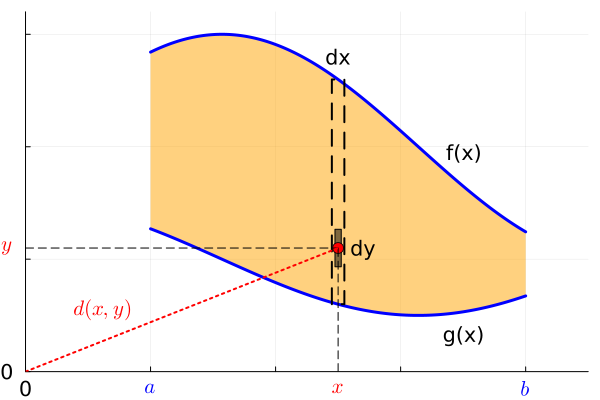
\includegraphics[width=0.6\columnwidth]{graphics/Chap06/MomentOfInertiaAboutZaxis.png}
    \caption[]{\textbf{(Moment of Inertia about the $\bm{z}$-Axis):} This figure illustrates how to use a rectangle of width $dx$, upper bounded by $f(x)$ and lower bounded by $g(x)$, to compute the moment of inertia about the $z$-axis, that is, the axis perpendicular to the $(x,y)$-plane and passing through the origin. The body is assumed to be of constant density. The computation requires two integrals. The first one, along the $y$-direction, is a very simple computation of the moment of inertia of an infinitesimally thin rectangle of width $dx$. The second one, along the $x$-direction, adds up the contribution of each thin rectangle. The final result is given in \eqref{eq:MomentInertiaAnoutZaxis}.}
    \label{fig:MomentInertiaAnoutZaxis}
\end{figure}

\subsection{Moment of Inertia}

This is a repeat of Section~\ref{sec:MoementInertiaFirstTime}, with the idea that you may be more interested in it now.\\

The \textbf{moment of inertia} (\( I \)) of an object about a specific axis is a measure of how difficult it is to change the rotational motion of that object. It depends on the mass distribution of the object relative to the axis of rotation. The moment of inertia is given by the integral

\[
I = \int r^2 \, dm,
\]

where \( r \) is the distance of a small mass element (\( dm \)) from the axis of rotation. This formula highlights that the further the mass is distributed from the axis, the higher the moment of inertia, thus making it harder to rotate the object.

For practical applications, common shapes have standard formulas for their moments of inertia. For example, for a solid cylinder of radius \( R \) rotating about its central axis, the moment of inertia is
\[
I = \frac{1}{2} mR^2,
\]
where \( m \) is the mass of the cylinder. This value helps in understanding the rotational characteristics of the cylinder and plays a crucial role in dynamics and engineering.
\\

\begin{propColor}{Moment of Inertia about the $\bm{z}$-Axis for Planar Bodies of Constant Density}{MomentInertia}

Given the planar body in Fig.~\ref{fig:MomentInertiaAnoutZaxis} bounded by \(y = f(x)\) and \(y = g(x)\), with constant density \(\rho\), the moment of inertia about the \(z\)-axis can be computed by a single integral from \(x = a\) to \(x = b\),
\begin{equation}
\label{eq:MomentInertiaAnoutZaxis}
 I_z = \int_a^b \rho \left( x^2(f(x) - g(x)) + \frac{1}{3} (f^3(x) - g^3(x)) \right) dx.   
\end{equation}
   
\end{propColor}

\textbf{Proof:} The proof is another example of the power of the rectangle in solving Calculus problems. Please refer to Fig.~\ref{fig:MomentInertiaAnoutZaxis} throughout the derivation.\\

Consider the vertical rectangle of width $dx$, and then within the rectangle, a small rectangle of height $dy$. The differential area of the infinitesimal rectangle is the product of height times width, that is, $dA := dy\, dx$ and the differential mass is the product of the density $\rho$ times the differential area, giving us
\begin{equation}
    dm = \rho \, dA = \rho \, dy \, dx.
\end{equation}
The differential moment of inertia about the $z$-axis is defined to be the distance squared times the differential mass, where 
$$r^2 = d^2(x, y) = x^2 + y^2.$$
We need to add up the contribution of each differential mass along the $y$-axis of the thin rectangle, which results in the integral
\begin{equation}
\begin{aligned}
    dI_z(x) &= \left[\int_{g(x)}^{f(x)} d^2(x,y) \rho \,  dy \right] dx ~~(\text{integral w.r.t.}~~y)\\[1em]
    & =  \left[\int_{g(x)}^{f(x)} (x^2 + y^2) \rho \,  dy \right] dx ~~(x~\text{is treated like a constant when integrating w.r.t.}~~y)\\[1em]
    & = \left[ x^2 \, y + \frac{y^3}{3}   \right]_{g(x)}^{f(x)}~~ \rho \, dx \\[1em]
    & = \left( x^2(f(x) - g(x)) + \frac{1}{3} (f^3(x) - g^3(x)) \right) ~~ \rho \, dx.
\end{aligned}    
\end{equation}
Next, we need to integrate with respect to $x$ so as to add up the contribution of each thin rectangle because that is how Calculus works!
\begin{equation}
    \begin{aligned}
        I_z & = \int_a^b dI_z(x) \\[1em]
        & =\int_a^b \left( x^2(f(x) - g(x)) + \frac{1}{3} (f^3(x) - g^3(x)) \right) ~~ \rho \, dx,
    \end{aligned}
\end{equation}
which establishes \eqref{eq:MomentInertiaAnoutZaxis}.
\Qed

\bigskip


\emstat{\textbf{Suggested Videos:}
\begin{itemize}
\item \href{https://youtu.be/lwO0V5FitAo}{More on moment of inertia | Moments, torque, and angular momentum} by Khan Academy.
\item \href{https://youtu.be/lNx0yPdl960}{Demonstrating Rotational Inertia (or Moment of Inertia)} by Flipping Physics. It's a bit goofy but full of information if you can stick through it. It's also a bit advanced.
\item \href{https://www.youtube.com/watch?v=-slWe0Ev7zc}{Moment of Inertia} by DoctorPhys. This is Lesson 1 of many! Next, we call out Lesson 9 because it pertains to the BallBot.
    \item \href{https://www.youtube.com/watch?v=olPyUlRLMyg}{Moment of Inertia for a Spherical Shell} by DoctorPhys. This is the moment of inertia of a basketball rolling on a floor.
\end{itemize}}


\begin{figure}[htb]%
    \centering
\subfloat[]{%
	\centering
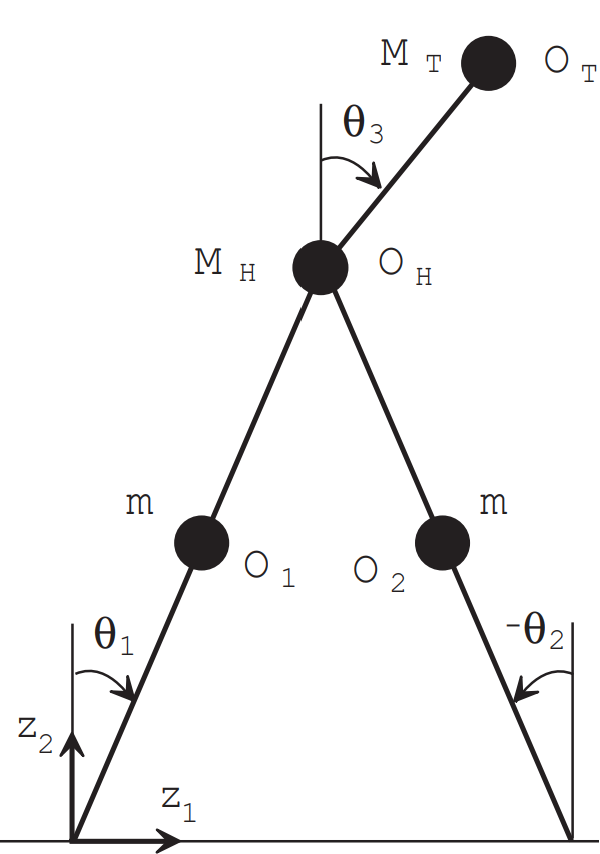
\includegraphics[height=0.45\columnwidth]{graphics/Chap06/3LinkWalkerFrom1999.png}
}%
\hspace{35pt}%
\subfloat[]{%
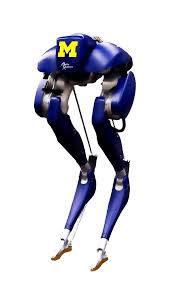
\includegraphics[height=0.45\columnwidth]{graphics/Chap06/Cassie.jpeg}}%
\centering
\hspace{35pt}%
\subfloat[]{%
    %
	\centering
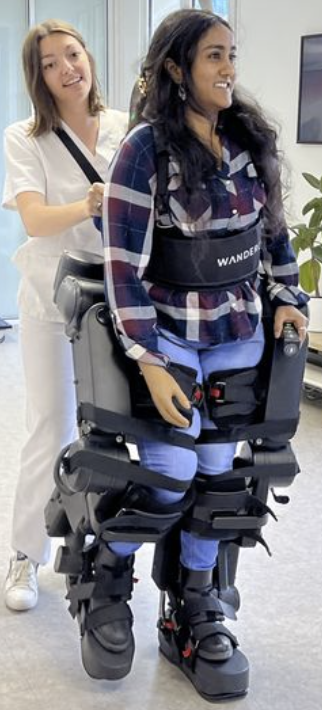
\includegraphics[height=0.45\columnwidth]{graphics/Chap06/Atalante.png}}%
    \caption[]{Michigan's foray into bipedal locomotion began with the study of the 3-link walker shown in (a), and over the years, progressed to Cassie in (b), and collaborating with \href{https://en.wandercraft.eu/}{Wandercraft} on the exoskeleton, Atalante, shown in (c). Atalante allows patients with paraplegia to walk again. In addition to powering the patient's legs, it provides the overall balance for the patient and itself. It is truly a wearable robot.}
    \label{fig:3LinkWalker}
\end{figure}

\subsection{A Simple Planar Biped}

Most of the terms in the model are defined in Fig.~\ref{fig:3LinkWalker}-(a). Missing is the length of the torso (line from $O_H$ to $O_T$) is $L$ and the four line segments in the legs each have length $r$.\\

\begin{lstlisting}[language=Julia,style=mystyle]
# Julia code
using Symbolics

# 3-link Walker Model is from 1999. 
# All angles are ABSOLUTE and are
# Positive in the CW Direction (not CCW)

# Variable declarations
@variables th1 th2 th3 dth1 dth2 dth3 m Mh Mt g L r

# Generalized coordinates
q = [th1, th2, th3]

# First derivative of generalized coordinates
dq = [dth1, dth2, dth3]


# Position of masses in the system
p_m1 = [r/2*sin(th1), r/2*cos(th1)]
p_Mh = [r*sin(th1), r*cos(th1)]
p_Mt = p_Mh + [L*sin(th3), L*cos(th3)]
p_m2 = p_Mh - [r/2*sin(th2), r/2*cos(th2)]

# Potential energy of masses in the system
PE_m1 = p_m1[2] * m * g
PE_Mh = p_Mh[2] * Mh * g
PE_Mt = p_Mt[2] * Mt * g
PE_m2 = p_m2[2] * m * g

# Total potential energy of the system
PE = PE_m1 + PE_Mh + PE_Mt + PE_m2
PE = Symbolics.simplify(PE)

# Velocities of masses in the system
v_m1 = Symbolics.jacobian(p_m1, q) * dq
v_Mh = Symbolics.jacobian(p_Mh, q) * dq
v_Mt = Symbolics.jacobian(p_Mt, q) * dq
v_m2 = Symbolics.jacobian(p_m2, q) * dq

# Kinetic Energy of each mass on the Robot
KE_m1 = 0.5 * m * sum(v_m1.*v_m1) 
KE_Mh = 0.5 * Mh * sum(v_Mh.*v_Mh)
KE_Mt = 0.5 * Mt * sum(v_Mt.*v_Mt)
KE_m2 = 0.5 * m * sum(v_m2.*v_m2)

# Total kinetic energy of the system
KE = KE_m1 + KE_Mh + KE_Mt + KE_m2
KE = Symbolics.simplify(KE)

# Form the Lagrangian
L = KE - PE

# Compute terms in the Robot Equations
G = Symbolics.gradient(PE, q)
D = Symbolics.hessian(KE, dq) # Strange name explained below

# Compute C (advanced, uses Christoffel symbols)
n = length(q)
C = Array{Num}(undef, n, n) # Num is Symbolic Type 
                             # Strange name explained below
for k in 1:n
    for j in 1:n
        C[k, j] = 0
        for i in 1:n
            C[k, j] += 0.5 * (Symbolics.gradient(D[k, j], q)[i] + 
            Symbolics.gradient(D[k, i], q)[j] - Symbolics.gradient(D[i, j], q)[k]) * dq[i]
        end
    end
end

# Place an actuator at the hip on 
# the relative angle between the torso and 
# each leg
# Use D'Alembert's Principle 
E = [th3-th1; th3-th2] 
B = Symbolics.jacobian(E, q)
B = B'
JacG = Symbolics.jacobian(G, q) # Used when we discuss lienearization of NL models



# Only run simple after all Symbolic manipulation is done and you 
# are ready to create a function
if true
    # Simplify as much as possible at the very end
    D = simple(D)
    C = simple(C)
end


# Create a function that computes all terms
# in the Robot Equations
fcn_name = "dyn_mod_3LinkWalker"
modelParamString = "g, r, L, m, Mh, Mt = modelParameters3LinkWalker()"
# Need to include line break command \n
variableNamesString = "th1, th2, th3 = q \ndth1, dth2, dth3 = dq"
writeEOM(fcn_name, D, C, G, B, JacG,modelParamString,variableNamesString)

# bring the model into the workspace for later use
include("dyn_mod_3LinkWalker.jl") 


# If the line above fails, it is because Julia is trying to read the file before it has 
# been made available to it by the file system. Simply copy the command into a new cell and 
# run it. The time it takes you to do that will allow the file system to catch up! :-)
\end{lstlisting}
\textbf{Output} 
\begin{verbatim}
[creating DYN_MOD_3LINKWALKER.jl]
File dyn_mod_3LinkWalker.jl created successfully!
dyn_mod_3LinkWalker (generic function with 1 method)
\end{verbatim}

\bigskip

Here is the Lagrangian Model.

\bigskip

\begin{lstlisting}[language=Julia,style=mystyle]
function modelParameters3LinkWalker()
#
    r=1;   # length of each leg
    m=5;   # mass of a leg
    Mh=15; # mass of hips
    Mt=10; #mass of torso
    L=0.5; # distance between hips and torso mass
    g=9.8; # acceleration due to gravity
#    
    return  g, r, L, m, Mh, Mt
end


function dyn_mod_3LinkWalker(q, dq)
# DYN_MOD_3LINKWALKER
# 2024-02-21 17:48:08
#
# Author: Grizzle
#
# Model NOTATION: D(q)ddq + C(q,dq)*dq + G(q) = B*tau 
# The Robot Equations: From Lagrange's Equations of Motion
#
g, r, L, m, Mh, Mt = modelParameters3LinkWalker()
#
# Variable names for the model
th1, th2, th3 = q 
dth1, dth2, dth3 = dq
#
D = zeros(3, 3)
  D[1, 1] = r^2*(Mh + Mt + 5*m/4)
  D[1, 2] = -0.5*m*r^2*cos(th1 - th2)
  D[1, 3] = L*Mt*r*cos(th1 - th3)
  D[2, 1] = -0.5*m*r^2*cos(th1 - th2)
  D[2, 2] = 0.25*m*r^2
  D[2, 3] = 0
  D[3, 1] = L*Mt*r*cos(th1 - th3)
  D[3, 2] = 0
  D[3, 3] = L^2*Mt
#
C = zeros(3, 3)
  C[1, 1] = 0.0
  C[1, 2] = -0.5*dth2*m*r^2*sin(th1 - th2)
  C[1, 3] = L*Mt*dth3*r*sin(th1 - th3)
  C[2, 1] = 0.5*dth1*m*r^2*sin(th1 - th2)
  C[2, 2] = 0.0
  C[2, 3] = 0.0
  C[3, 1] = -L*Mt*dth1*r*sin(th1 - th3)
  C[3, 2] = 0.0
  C[3, 3] = 0.0
#
G = zeros(3)
  G[1] = -Mh*g*r*sin(th1) - Mt*g*r*sin(th1) - (3/2)*g*m*r*sin(th1)
  G[2] = (1/2)*g*m*r*sin(th2)
  G[3] = -L*Mt*g*sin(th3)
#
B = zeros(3, 2)
  B[1, 1] = -1
  B[2, 2] = -1
  B[3, 1] = 1
  B[3, 2] = 1
#
JacG = zeros(3, 3)
  JacG[1, 1] = -Mh*g*r*cos(th1) - Mt*g*r*cos(th1) - (3/2)*g*m*r*cos(th1)
  JacG[2, 2] = (1/2)*g*m*r*cos(th2)
  JacG[3, 3] = -L*Mt*g*cos(th3)
#
  return (D=D, C=C, G=G, B=B, JacG=JacG)
end
\end{lstlisting}


\section{(Optional Read:) Proof behind Lagrange Multipliers for Equality Constraints}


Let $f:\real^n \to \real$ be a differentiable cost function, $g_i:\real^n \to \real$ be differentiable equality constraints for $1 \le i \le m$, and let $x_0 \in \real^n$ be an arbitrary point. We seek necessary conditions for $x_0$ to be a local extremum of the constrained optimization problem \eqref{eq:GenericMultipleConstraintOptimizationProblem01}, which we repeat here for convenience,
\begin{equation}
\label{eq:GenericMultipleConstraintOptimizationProblem01Repeated}
\begin{aligned}
\text{Minimize} \quad & f(x)\\
\text{subject to} \quad & g_i(x) = 0, ~ 1\le i \le m,
\end{aligned}    
\end{equation}


We use the Jacobian to define $(n+1)$ constant row vectors
\begin{equation}
    \begin{aligned}
        J_f(x_0) := \frac{\partial f(x_0)}{\partial x} &= \left[ \begin{array}{cccc} \frac{\partial f(x_0) }{\partial x_1}& \frac{\partial f(x_0)}{\partial x_2}  & \cdots & \frac{\partial f(x_0)}{\partial x_n}\end{array} \right],  \medskip \\
        J_{g_i}(x_0):= \frac{\partial g_i(x_0)}{\partial x} &=  \left[ \begin{array}{cccc} \frac{\partial g_i(x_0) }{\partial x_1}& \frac{\partial g_i(x_0)}{\partial x_2}  & \cdots & \frac{\partial g_j(x_0)}{\partial x_n}\end{array} \right], ~1 \le i \le m.
    \end{aligned}
\end{equation}
By definition\footnote{Write $J_f(x_0) = \alpha_1 J_{g_1}(x_0) + \alpha_2 J_{g_2}(x_0) + \cdots + \alpha_m J_{g_m}(x_0)$, and then define $\lambda_i:= - \alpha_i$. Moving all the terms to the left side of the equation gives \eqref{eq:JacfLinearComoJacgi}.}, we note that $J_f(x_0)$ is a linear combination of the set of row vectors $\{ J_{g_1}(x_0), J_{g_2}(x_0), \ldots, J_{g_m}(x_0) \}$, if, and only if, there exist scalars $\lambda_1, \lambda_2, \ldots, \lambda_m \in \real$ such that
\begin{equation}
\label{eq:JacfLinearComoJacgi}
    J_f(x_0) + \lambda_1 J_{g_1}(x_0) + \lambda_2 J_{g_2}(x_0) + \cdots + \lambda_m J_{g_m}(x_0) =0.
\end{equation}
In other words, 
\begin{itemize}
    \item $J_f(x_0)$ being a linear combination of $\{ J_{g_1}(x_0), J_{g_2}(x_0), \ldots, J_{g_m}(x_0) \}$ will be intimately related to the existence of Lagrange multipliers transforming the constrained optimization problem \eqref{eq:GenericMultipleConstraintOptimizationProblem01Repeated} into the unconstrained problem of finding stationary points for the Lagrangian
\begin{equation}
\label{eq:Lagrangian4Proof}
    L(x, \lambda):= f(x) + \lambda_1 g_1(x) + \lambda_2 g_2(x) + \cdots + \lambda_m g_m(x).
\end{equation}

    \item We also note that the set of row vectors $\{ J_{g_1}(x_0), J_{g_2}(x_0), \ldots, J_{g_m}(x_0) \}$ is \textbf{linearly independent} if, and only if, the constraint qualification condition holds at $x_0$,
\begin{equation}
\label{eq:JacobianEqualityConstraintsFullRank}
    \rank \left( \frac{\partial g(x_0)}{\partial x} \right) =  \rank \left(  \left[ \begin{array}{c} 
   J_{g_1}(x_0)\\  
    J_{g_2}(x_0)\\
    \vdots \\
    J_{g_m}(x_0)
    \end{array} \right]\right) = m.
\end{equation}
\item The coefficients in \eqref{eq:JacfLinearComoJacgi} are unique if, and only if, the set of row vectors $\{ J_{g_1}(x_0), J_{g_2}(x_0), \ldots, J_{g_m}(x_0) \}$ is linearly independent.

\end{itemize}

We next state a result that makes it easy to relate conditions for $x_0$ being a local extremum of \eqref{eq:GenericMultipleConstraintOptimizationProblem01Repeated} to $x_0$ being a stationary point of the Lagrangian \eqref{eq:Lagrangian4Proof}.

\begin{propColor}{When can a Row Vector be Expressed as a Linear Combination of other Row Vectors}{DependentRowVectors} 
The row vector $J_f(x_0)$ is a linear combination of the set of row vectors $\{ J_{g_1}(x_0), J_{g_2}(x_0), \ldots, J_{g_m}(x_0) \}$ if, and only if,
\begin{equation}
\label{eq:DependentRowVectors}
 \bigcap_{i=1}^n \nullspace\left(  J_{g_i}(x_0) \right) \subset   \nullspace\left( J_f(x_0) \right).
\end{equation}    
\end{propColor}

We delay the proof of Prop.~\ref{thm:DependentRowVectors} until later.

\textbf{Assumptions:}
\begin{itemize}
    \item $x_0$ is feasible; that is $g_i(x_0)=0$, $1 \le i \le m$.
    \item $x_0$ satisfies the constraint qualification condition, that is, \eqref{eq:JacobianEqualityConstraintsFullRank} holds.
\end{itemize}

Given $x_0$ as above, we call $v\in \real^n$ a \textbf{feasible direction} if $v \in \bigcap_{i=1}^n \nullspace\left(  J_{g_i}(x_0) \right)$. Why this name? One way to understand it is that by the linear approximation of $g_i: \real^n \to \real$ at a feasible point $x_0$,
\begin{align*}
     g_i(x_0 + v) &\approx g_i(x_0) +  J_{g_i}(x_0) \cdot v\\
            & \approx J_{g_i}(x_0) \cdot v \\
            & \approx 0.
\end{align*}
Hence, if $x_0$ is feasible, then so is $x_0 + v$ to first order\footnote{A more formal formulation uses the concept of a \textbf{directional derivative}, defined as, for $v$ a unit vector, 
$$ \left. \frac{d}{dt} g_i(x_0 + t\cdot v)\right|_{t = 0} = \frac{\partial g_i(x_0)}{\partial x} \cdot v =  J_{g_i}(x_0) \cdot v.$$
Hence, the directional derivative vanishes for $v \in \nullspace\left(  J_{g_i}(x_0) \right)$.}. 

Let $v \in \bigcap_{i=1}^n \nullspace\left(  J_{g_i}(x_0) \right)$ be arbitrary, and consider $f(x_0 + v)$ through the lens of its linear approximation,
$$ f(x_0 + v)  \approx f(x_0) +  J_f(x_0) \cdot v. $$
From the linearization of $f$ at $x_0$, we make the following conclusions:
\begin{itemize}
    \item If $v \not \in \nullspace\left( J_f(x_0) \right)$, meaning $J_{f}(x_0) \cdot v \neq 0$, then we can move along $v$ to make $f(x_0 + v)$ smaller or larger than $f(x_0)$. In this case, $x_0$ is not an extreme point of \eqref{eq:GenericMultipleConstraintOptimizationProblem01Repeated}. 
    \item Therefore, the only way for $x_0$ to be an extreme point is for $J_{f}(x_0) \cdot v = 0$, that is  $v \in \nullspace\left( J_f(x_0) \right)$. 
\end{itemize}

\emstat{  
   \textcolor{black}{\bf Because $\displaystyle \bm{v} \in \bigcap \bm{_{i=1}^n \nullspace\left(  J_{g_i}(x_0) \right)} $ was arbitrary, we conclude that the only way for $\bm{x_0$} to be an extreme point of \eqref{eq:GenericMultipleConstraintOptimizationProblem01Repeated} is 
   for \eqref{eq:DependentRowVectors} to hold, and thus $\bm{J_f(x_0)}$ can be expressed as the linear combination   
\begin{equation}
\label{eq:OurStationaryCondition}
  \bm{ J_f(x_0) + \lambda_1 J_{g_1}(x_0) + \lambda_2 J_{g_2}(x_0) + \cdots + \lambda_m J_{g_m}(x_0) =0. }
\end{equation}
}
}

We are now essentially done, with only some bookkeeping to complete the proof. Using the coefficients in \eqref{eq:OurStationaryCondition}, define the Lagrangian as in \eqref{eq:Lagrangian4Proof}. 
Then, by \eqref{eq:OurStationaryCondition}, $x_0$ is a stationary point of $L$.\\

That seems almost too easy! But it was easy only because we knew about Prop.~\ref{thm:DependentRowVectors} for checking that a given row vector could be expressed as a linear combination of other row vectors. Knowledge is power. 

\Qed

\textbf{ Proof of Prop.~\ref{thm:DependentRowVectors} } Without loss of generality, we can assume that the set of row vectors $\{ J_{g_1}(x_0), J_{g_2}(x_0), \ldots, J_{g_m}(x_0) \}$ is linearly independent because any dependent vectors do not change the intersection of their null spaces.

If there exist $\lambda_1, \ldots, \lambda_m$ such that \eqref{eq:JacfLinearComoJacgi} holds, then $v$ satisfying $J_{g_i}(x_0) \cdot v = 0$, $1 \le i \le m$, implies 
$J_f(x_0) \cdot v=0.$ For the other direction, we assume that $\{ J_{g_1}(x_0), J_{g_2}(x_0), \ldots, J_{g_m}(x_0) \}$ is linearly independent and that $J_f(x_0)$ is not a linear combination of these vectors. Hence, the $ (m+1)\times n$ matrix
$$A:= \left[ \begin{array}{c} 
J_f(x_0) \\
   J_{g_1}(x_0)\\  
    J_{g_2}(x_0)\\
    \vdots \\
    J_{g_m}(x_0)
    \end{array} \right] $$
    has full row rank. Therefore, there exist $v\in \real^n$ such that 
    $$A \cdot v = \left[ \begin{array}{c} 
1\\
   0\\  
    0\\
    \vdots \\
    0
    \end{array} \right].$$
    Hence, there exists $v \in  \bigcap_{i=1}^n \nullspace\left(  J_{g_i}(x_0) \right) $ such that $v \not \in \nullspace\left( J_f(x_0) \right)$. This completes the proof.
    \Qed
\bigskip

\section{(Optional Read:) Proof Underlying Gradient Descent with Equality Constraints}

It is a bit ironic, but the above proof of the Method of Lagrange Multipliers shows how to accomplish constrained optimization without explicitly computing Lagrange multipliers! In fact, it shows how to update gradient descent to work in the presence of equality constraints. We retain all of the assumptions made for the proof of the Method of Lagrange Multipliers with Equality Constraints.

\begin{methodColor}{Gradient Descent with Equality Constraints}{GradientDescentWithEqualityConstraints} 

Consider the constrained optimization problem \eqref{eq:GenericMultipleConstraintOptimizationProblem01} for functions $f:\real^n \to \real$ and $g:\real^n \to \real^m$ with optimal value $x^\ast$. If the columns vectors from the  gradients $\{ \nabla g_1(x^\ast),  \nabla g_2(x^\ast), \ldots,  \nabla g_m(x^\ast)\}$ are linearly independent  (equivalently, the rows of the Jacobian $\frac{ \partial g(x^\ast)}{\partial x} $ are linearly independent), then a locally optimal $x^\ast$ 
can be found as follows: \\


\textbf{Initialization:} Find a feasible point $x_0\in \real^n$, that is, a point such that $g_i(x_0) = 0$ for $1 \le i \le m$. This can be accomplished with \texttt{NLsolve}.

\bigskip

\textbf{Loop:} Given a point $x_k \in \real^n$, repeat the following steps to either find $x_{k+1}$ or terminate.

\begin{enumerate}
\renewcommand{\labelenumi}{(\alph{enumi})}
\setlength{\itemsep}{.2cm}

    \item \textbf{Compute:} $\nabla f(x_k)$, the gradient of $f$ at $x_k$ and $\frac{\partial g(x_k)}{\partial x}$, the Jacobian of the constraint vector. \\

  From the proof of the Method of Lagrange Multipliers, the set of feasible directions is
    $$V:= \bigcap_{i=1}^n \nullspace\left(  J_{g_i}(x_k) \right) = \nullspace \left(\frac{\partial g(x_k)}{\partial x}\right),$$  where $g:\real^n \to \real^m$ is the vector of equality constraints. \\
    
    \textcolor{blue}{\bf Wow, it's good to know about null spaces. They are not just abstract nonsense after all!}\\

   \item \textbf{Compute the orthognal projection of $\bm{\nabla f(x_k)}$ onto $\bm{V}$, the set of feasible directions:}  
   This can be accomplished by applying Gram-Schmidt. Indeed, let $\{b_1, b_2, \ldots, b_m\}$ be an orthonormal basis for the columns of $\left( \frac{\partial g(x_k)}{\partial x} \right)^\top$. Then
    $$P^V_{\nabla f(x_k)}:= \nabla f(x_k) - \sum_{i=1}^m \left(\nabla f(x_k) \bullet b_i \right)\cdot b_i $$
    is the desired projection. \\
    
    \textbf{Why:} Each term $\left(\nabla f(x_k) \bullet b_i \right)\cdot b_i$ is a component of $\nabla f(x_k)$ that is orthogonal to $V$, the feasible directions. From ROB 101 \textit{Computational Linear Algebra}, Chapter 9, once these components are subtracted off, only the part of $\nabla f(x_k)$ lying in $V$ is left.\\

      \textcolor{blue}{\bf Wow, it's good to know about Gram-Schmidt and orthogonal vectors. Like null spaces, these are very useful tools}.

    \item \textbf{Update or Terminate, That is the Question:} If the termination condition is not met, define
    $$x_{k+1} = x_k - s \cdot P^V_{\nabla f(x_k)},$$
    where $s>0$ is the step size. Loop back to (a).

    \item \textbf{Termination Condition:} $||P^V_{\nabla f(x_k)}|| < a_{\rm tol}$; in other words, $J_f(x_k)$ is to numerical precision a linear combination of $\{ J_{g_1}(x_k),  J_{g_2}(x_k), \ldots,  J_{g_m}(x_k)\}$, and thus  $x_k$ is (to numerical precision) a stationary point of the Lagrangian.
\end{enumerate}


\textbf{Notes:} 
\begin{itemize}
    \item In practice, the updates $x_k$ will ``slowly'' exit the feasible set. Hence, when $||g(x_k)||$ exceeds a user-defined tolerance, a new call to \texttt{NLsolve} should be made. 
    \item Lagrange likely understood that an algorithm like this was possible, but given that his ``computer'' consisted of pen and paper, it was not feasible to pursue this version of his method.
    \item If there are no constraints, then the null space of $\left( \frac{\partial g(x_k)}{\partial x} \right)$ is all of $\real^n$. The projected gradient is then the regular gradient. 
    \item An algorithm like this one cannot be presented in most Calc III courses  \textbf{because Linear Algebra traditionally comes after Calc I through Calc IV}. Michigan Robotics is pushing to reverse this sequence and put Linear Algebra before Calculus. 
    \item \textbf{\texttt{JuMP} does all of this and a whole lot more}. It is your best option for use in professional projects. For learning about gradient descent, the workhorse of Machine Learning (ML), algorithms like the one presented here are helpful.
\end{itemize}   
\end{methodColor}

Here is an instantiation of the above version of Lagrange's Method for Optimization with Equality Constraints. 

\begin{lstlisting}[language=Julia,style=mystyle]
using ForwardDiff, LinearAlgebra, NLsolve

# Define the cost function f(x) and the equality constraints G(x)
function f(x)
    return x[1]^2 + x[2]^2 + x[3]^2 + x[4]^2
end

function G(x)
    return [x[1] + x[2] - 3, sin(pi*x[1]) - x[3]^2 - 1 + x[4]^3]
end

# Compute the gradient of f and the Jacobian of G using ForwardDiff
grad_f(x) = ForwardDiff.gradient(f, x)
JacG(x) = ForwardDiff.jacobian(G, x)

# Define functions used for computing the projection of grad_f onto 
# the nullspace of JacG, that is, onto the feasible directions

function gram_schmidt(jacobian_G)
    n, m = size(jacobian_G)
    B = zeros(n, m)  # Basis vectors

    for j = 1:m
        b = jacobian_G[:, j]
        for i = 1:j-1
            b -= dot(B[:, i], jacobian_G[:, j]) * B[:, i]
        end
        B[:, j] = b / norm(b)
    end

    return B
end

# Project the gradient onto the feasible directions, 
# that is, nullspace of JacG
function project_grad_f(grad_f, B)
    # Iterate over columns of B, subtracting their projection from grad_f
    projected_grad_f = grad_f
    for j = 1:size(B, 2)
        projected_grad_f = projected_grad_f - dot(grad_f, B[:, j]) * B[:, j]
    end
    return projected_grad_f
end


# Function to find a feasible starting point using NLsolve
# or to push xk back onto the feasible set when it 
# drifts off
function find_feasible_start(G, x_guess)
    # build functin for NLSolve
    function constraint!(F, x)
        F[1:2] = G(x)
    end
    xFeasible = nlsolve(constraint!, x_guess)
    return xFeasible.zero
end
#
## End define functions for projected gradient descent

## Actual Gradient Descent Algorithm Starts Here

x_guess = [0.0, 0.0, 0.0, 0.0] # Not feasible
x0 = find_feasible_start(G, x_guess) # Make feasible


# set step size, maxIter, tolerances
s=0.1
maxIter=10000
gradTol = 1e-6
constraintTol = 1e-4

xk = x0
for k=1:maxIter
    jacobian_G_transposed = transpose(JacG(xk))
    B = gram_schmidt(jacobian_G_transposed)
    projected_grad_f = project_grad_f(grad_f(xk), B)
    if norm(projected_grad_f) < gradTol
        println("---- Iteration $k ----")
        println("Met tolerance.")
        println("Jacf applied to null(JacG) (should be near 0): ", 
           round.((grad_f(xk)')*nullspace(JacG(xk)), digits=5))
        println("Constraints (should be near 0): ", round.(G(xk), digits=5))
        println("----------------- ")
        break
    else
        # Update
        xk = xk - s*projected_grad_f
    end
    if norm(G(xk)) > constraintTol
        xk = find_feasible_start(G, xk) # Again Feasible
    end
end
xStar = xk
fStar = f(xStar)

println("\nFinal Results:")
println("-----------------")
println("Optimal x: ", round.(xStar, digits=5))
#
println("Optimal Cost f(xStar): ", round(fStar, digits=5))

\end{lstlisting}
\textbf{Output} 
\begin{verbatim}
---- Iteration 184 ----
Met tolerances.
Jacf applied to null(JacG) (should be near 0): [0.0 -0.0]
Constraints (should be near 0): [-0.0, 2.0e-5]
----------------- 

Final Results:
-----------------
Optimal x: [0.95451, 2.04549, 0.0, 0.95008]
Optimal Cost f(xStar): 5.99778
\end{verbatim}

% \begin{lstlisting}[language=Julia,style=mystyle]

% \end{lstlisting}
% \textbf{Output} 
% \begin{verbatim}



\section{Words of Wisdom from one of the Planet's Greatest Living Mathematicians}

\href{https://youtube.com/shorts/k2QVCfoW7uI?si=vhh7jRLSrJoGpHjz}{\bf Math isn't actually Sorcery} \textbf{by Prof. Terrence (Terry) Tao}, an Australian-American mathematician who is widely regarded as one of the greatest living mathematicians (if you hear an accent in the video, it's Aussie). \\

Summarized from \href{https://en.wikipedia.org/wiki/Terence_Tao}{Wikipedia}: Born in 1975 to Chinese immigrant parents in Adelaide, Tao was a child prodigy who exhibited extraordinary mathematical abilities from a very young age. \textbf{He skipped six grades and attended university-level mathematics courses at age 9.} At just eight years old, he scored 760 on the SAT math section, a feat achieved by only three children in the history of the Johns Hopkins Study of Exceptional Talent program.\\

Tao's prodigious talent was further demonstrated through his participation in the International Mathematical Olympiad. He became the youngest participant in the competition's history, winning bronze, silver, and gold medals at ages 10, 11, and 13, respectively. He remains the youngest winner of each medal type in the Olympiad's history.\\


Currently, Tao is a professor of mathematics at the University of California, Los Angeles (UCLA), where he holds the James and Carol Collins Chair in the College of Letters and Sciences. His research spans various areas of mathematics, including harmonic analysis, partial differential equations, combinatorics, probability theory, and analytic number theory.\\

Tao's contributions to mathematics have earned him numerous prestigious awards, including the Fields Medal in 2006, the Royal Medal and Breakthrough Prize in Mathematics in 2014, and a MacArthur Fellowship in 2006. He has authored or co-authored over three hundred research papers, solidifying his reputation as one of the most influential mathematicians of his generation.\\

\emstat{
\textbf{Relevance to Calculus for the Modern Engineer:} At each step of our adventure, we've broken a new topic into smaller building blocks from which we could assemble an approach to solving a problem. Often, the building blocks, put end-to-end, formed an algorithm. Other times, they provided an Ah Ha moment of insight into how a complicated looking formula was a direct consequence of understanding rectangles (e.g., theory of integration and its applications) or linear approximations of functions (e.g., derivation of differentiation rules and the applications of derivatives, scalar and vector). Limits of one kind or another have been the cement holding the blocks together. 
}










